% Chapter 2

\chapter{Background and Literature Review} % Main chapter title

\label{Chapter2} % For referencing the chapter elsewhere, use \ref{Chapter1} 

\lhead{Chapter 2. \emph{Background and Literature Review}}

%----------------------------------------------------------------------------------------

This chapter starts by introducing the essential technical and conceptual aspects of RL in Section \ref{back}. Those basic concepts will then be used to build our controller implementation in the following chapters of this dissertation. In Section \ref{rlaracing}, we will then look at the literature regarding model-free RL algorithms in both discrete and continuous action space. Next, in Section \ref{nns}, we introduce the main concepts of convolutional neural networks, which are one of the main components of our Deep RL controllers. Finally, in Section \ref{rosandf1tenth} we will look at how to apply those algorithms to autonomous racing using ROS and the F1Tenth system and simulator. \newline
Our goal in this chapter is to start by explaining the basic ideas of RL and NNs to be then able to explain the more sophisticated algorithms that will be implemented in ROS on the F1Tenth platform. \newline

\section{Reinforcement Learning essentials}
\label{back}
\subsection{What is Reinforcement Learning}
Reinforcement Learning is a subfield of Machine Learning concerned with the problem of an agent that must learn behaviour through trial and error interactions with a changing environment. RL is one of four main ML paradigms (\cite{Alloghani2020}):
\begin{itemize}
	\item \textbf{Unsupervised learning} is a machine learning paradigm concerned with grouping data and finding patterns without any label provided. It is mainly used for solving problems related to clustering, compressing and filtering data and estimating statistical distributions.
	\item Different from unsupervised learning, \textbf{supervised learning} relies on labelled data to perform classification and prediction using various algorithms such as regressions, Bayesian networks and decision trees. The inconvenience with supervised learning is that the training dataset needs to be labelled, which is a very time-consuming task.
	\item \textbf{Semi-supervised learning} is a compromise between supervised and unsupervised learning: the training dataset comprises a majority of unlabelled data samples with a small number of labelled data samples. It is used when the cost of labelling the whole dataset for supervised learning is too high, but having some labelled data offers a significantly improved learning accuracy over unsupervised learning.
	\item Finally, \textbf{reinforcement learning} is the paradigm we will look at more in detail in the following paragraphs.
\end{itemize}


The increasing popularity of RL has been attributed mainly to the so-called deep learning revolution that started in 2012 and has since transformed the AI field (\cite{sejnowski2018deep}). \newline
The RL paradigm is presented in Figure \ref{rlparadigm}. At each time step $t$, an agent is changing the state of its environment through an action $a_t$, and thus finds itself in a new state $s_{t+1}$ after receiving the reward $r_{t+1}$. The agent has its own representation of the environment, which may be different from the actual state of the environment and follows an action selection policy. \newline
In many ways, reinforcement learning differs from the other main ML field of supervised learning. The main difference is that the agent does not need to be told what action would have been optimal after making an action. This is why RL can be used in several real-world situations when the optimal actions are unknown. Furthermore, unlike supervised learning, the RL agent can face a dynamic environment. 

\begin{figure}[H]
\centering
\tikzset{rlparadigm/.style={line width=0.75pt}} %set default line width to 0.75pt 
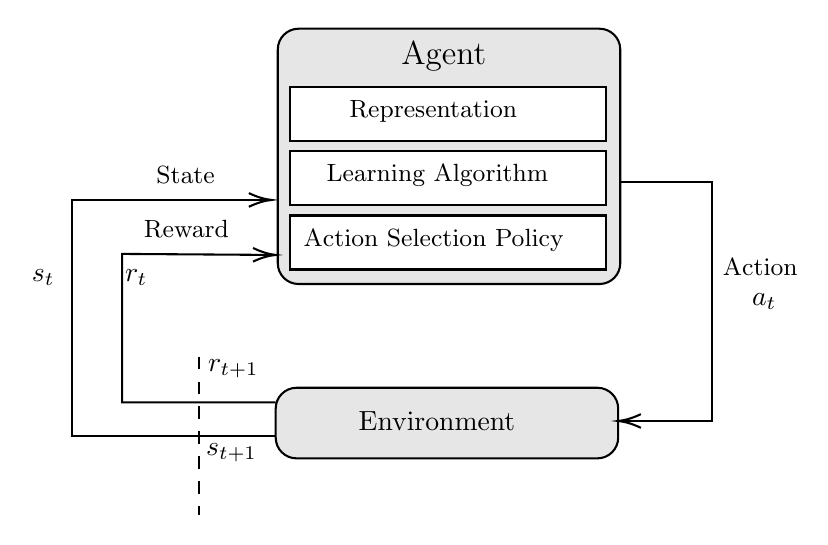
\begin{tikzpicture}[x=0.75pt,y=0.75pt,yscale=-1,xscale=1]
\draw  [fill={rgb, 255:red, 230; green, 230; blue, 230 }  ,fill opacity=1 ] (239,32) .. controls (239,26.48) and (243.48,22) .. (249,22) -- (394,22) .. controls (399.52,22) and (404,26.48) .. (404,32) -- (404,135) .. controls (404,140.52) and (399.52,145) .. (394,145) -- (249,145) .. controls (243.48,145) and (239,140.52) .. (239,135) -- cycle ;
%Shape: Rectangle [id:dp16443948240843453] 
\draw  [fill={rgb, 255:red, 255; green, 255; blue, 255 }  ,fill opacity=1 ] (245,50) -- (397,50) -- (397,76) -- (245,76) -- cycle ;
%Shape: Rectangle [id:dp4711312134028234] 
\draw  [fill={rgb, 255:red, 255; green, 255; blue, 255 }  ,fill opacity=1 ] (245,81) -- (397,81) -- (397,107) -- (245,107) -- cycle ;
%Shape: Rectangle [id:dp07379621845507045] 
\draw  [fill={rgb, 255:red, 255; green, 255; blue, 255 }  ,fill opacity=1 ] (245,112) -- (397,112) -- (397,138) -- (245,138) -- cycle ;
%Shape: Rectangle [id:dp569623469762901] 
\draw  [fill={rgb, 255:red, 230; green, 230; blue, 230 }  ,fill opacity=1 ] (238,205) .. controls (238,199.48) and (242.48,195) .. (248,195) -- (393,195) .. controls (398.52,195) and (403,199.48) .. (403,205) -- (403,219) .. controls (403,224.52) and (398.52,229) .. (393,229) -- (248,229) .. controls (242.48,229) and (238,224.52) .. (238,219) -- cycle ;
%Straight Lines [id:da0773786200794524] 
\draw    (238,202) -- (164,202) -- (164,130.5) -- (236,130.99) ;
\draw [shift={(238,131)}, rotate = 180.39] [color={rgb, 255:red, 0; green, 0; blue, 0 }  ][line width=0.75]    (10.93,-3.29) .. controls (6.95,-1.4) and (3.31,-0.3) .. (0,0) .. controls (3.31,0.3) and (6.95,1.4) .. (10.93,3.29)   ;
%Straight Lines [id:da1193665403379629] 
\draw    (404,96) -- (448,96) -- (448,211) -- (405,211) ;
\draw [shift={(403,211)}, rotate = 360] [color={rgb, 255:red, 0; green, 0; blue, 0 }  ][line width=0.75]    (10.93,-3.29) .. controls (6.95,-1.4) and (3.31,-0.3) .. (0,0) .. controls (3.31,0.3) and (6.95,1.4) .. (10.93,3.29)   ;
%Straight Lines [id:da20118699009626395] 
\draw  [dash pattern={on 4.5pt off 4.5pt}]  (201,180) -- (201,256.5) ;
%Straight Lines [id:da6333445083775118] 
\draw    (238,218.25) -- (140,218.25) -- (140,104.5) -- (234,104.5) ;
\draw [shift={(236,104.5)}, rotate = 180] [color={rgb, 255:red, 0; green, 0; blue, 0 }  ][line width=0.75]    (10.93,-3.29) .. controls (6.95,-1.4) and (3.31,-0.3) .. (0,0) .. controls (3.31,0.3) and (6.95,1.4) .. (10.93,3.29)   ;
% Text Node
\draw (297,27) node [anchor=north west][inner sep=0.75pt]   [align=left] {{\large Agent}};
% Text Node
\draw (272,55) node [anchor=north west][inner sep=0.75pt]  [font=\small] [align=left] {Representation};
% Text Node
\draw (261,86) node [anchor=north west][inner sep=0.75pt]  [font=\small] [align=left] {Learning Algorithm};
% Text Node
\draw (250,117) node [anchor=north west][inner sep=0.75pt]  [font=\small] [align=left] {Action Selection Policy};
% Text Node
\draw (276.5,205) node [anchor=north west][inner sep=0.75pt]   [align=left] {Environment};
% Text Node
\draw (452,131) node [anchor=north west][inner sep=0.75pt]  [font=\small] [align=left] {Action};
% Text Node
\draw (466,148) node [anchor=north west][inner sep=0.75pt]    {$a_{t}$};
% Text Node
\draw (173,113) node [anchor=north west][inner sep=0.75pt]  [font=\small] [align=left] {Reward};
% Text Node
\draw (164,136.5) node [anchor=north west][inner sep=0.75pt]    {$r_{t}$};
% Text Node
\draw (204,180) node [anchor=north west][inner sep=0.75pt]    {$r_{t+1}$};
% Text Node
\draw (179,87) node [anchor=north west][inner sep=0.75pt]  [font=\small] [align=left] {State};
% Text Node
\draw (119,136.5) node [anchor=north west][inner sep=0.75pt]    {$s_{t}$};
% Text Node
\draw (203,220.25) node [anchor=north west][inner sep=0.75pt]    {$s_{t+1}$};
\end{tikzpicture}
\caption{Reinforcement Learning Paradigm\textsuperscript{1}}
\small\textsuperscript{1} Unless stated otherwise, figures are my own work
\label{rlparadigm}
\end{figure}

The main categories of RL agents are presented in Figure \ref{taxonomy}. The fundamental distinction is whether or not the agent is given (or learns) a model of the environment, meaning a function predicting rewards and state transitions. A famous example of a model given RL algorithm is the AlphaGo/AlphaZero program, based on the Monte Carlo Tree Search method (MCTS), published in \cite{Silver2016MasteringTG}. However, apart when the agent plays a board game with simple rules, there is no environment model available for the agent, which means that the model has to be learned from experience: those algorithms are model learned. One of the issues with that method is that the agent could behave very well in his learning environment but terribly in the real one because of biases appearing during learning. An example of a model learned method is the Imagination-Augmented Agent (I2A), introduced in \cite{I2A}. \newline
The alternative to model-based is model-free: those methods tend to be more popular than model-based ones because they are often more easy to tune and implement. \newline
%https://ai.stackexchange.com/questions/4456/whats-the-difference-between-model-free-and-model-based-reinforcement-learning
It is important to note that model-based and model-free only refer to whether or not the agent uses predictions of the environment response (next reward and state) for the training. Those predictions could be either computed outside of the training algorithm, for example, by a program that understands the rules of a board game (model given) or learned by the agent in an approximate way (model learned). In the case of autonomous racing, model-based RL agents are still challenging to implement; however, \cite{modelbased} introduced a model-based controller using a deep neural network that sometimes performs even better than model-free state-of-the-art methods. That algorithm is model-learned and uses a simple Follow The Gap approach to generate training data to learn the model of the environment. \newline
 There are two main types of model-free algorithms: value-based and policy-based. The policy-based methods will focus on optimising policies; they can be either gradient-based or gradient-free. Gradient-based algorithms use gradient ascent to optimise the parameters of the policy. In contrast, gradient-free optimises a ``surrogate" objective function, like the Proximal Policy Optimization (PPO) introduced in \cite{ppo}. The value-based approach instead learns the state or the state-action value. Value-based methods can either evaluate and improve the same policy used for decision-making during learning (on-policy) or evaluate and improve a different policy than the one used for making actions. The most famous off-policy method is Q-Learning, which we will discuss in detail in Subsection \ref{qlearningsection}. From Q-Learning were introduced Deep Q Networks (DQN), discussed in Subsection \ref{dqlearningsection} and introduced in \cite{drl}. The Deep Deterministic Policy Gradient method, discussed in Subsection \ref{ddpgsection} was then introduced in \cite{ddpg2015} as a combination of policy and value-based approaches.

\begin{figure}[H]
\centering
\tikzset{every picture/.style={line width=0.75pt}} %set default line width to 0.75pt        

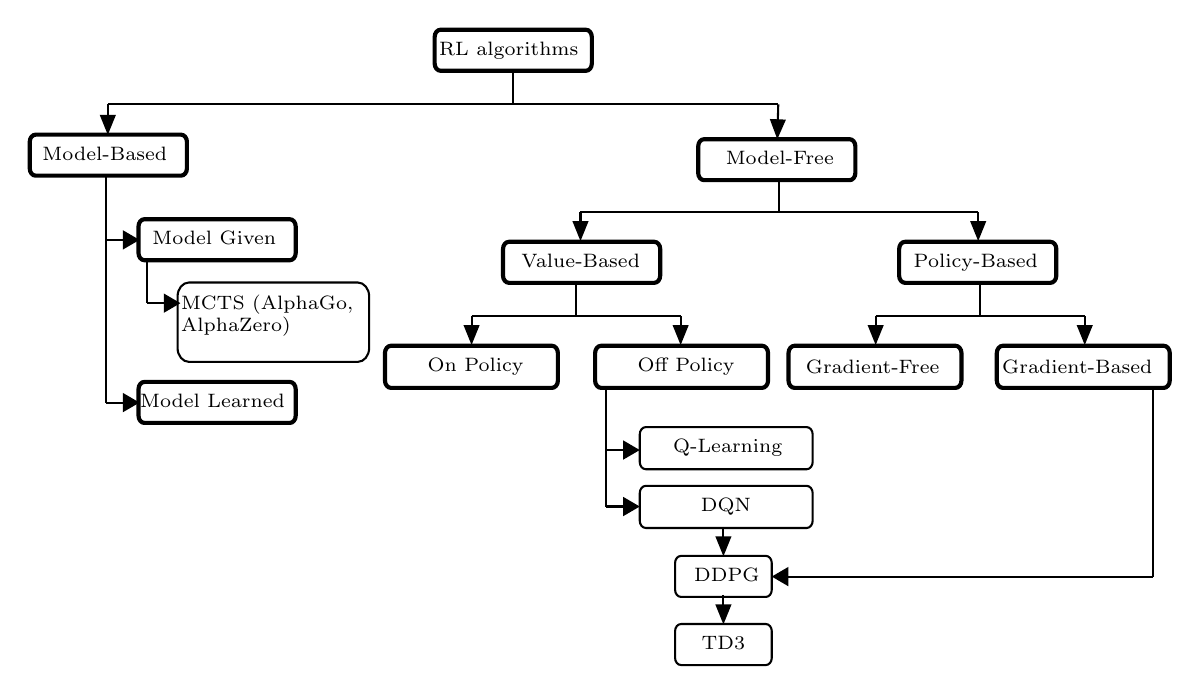
\begin{tikzpicture}[x=0.70pt,y=0.71pt,yscale=-1.15,xscale=0.96]
%uncomment if require: \path (0,300); %set diagram left start at 0, and has height of 300

%Flowchart: Alternative Process [id:dp40468518326516834] 
\draw  [line width=1.5]  (228.73,13.18) .. controls (228.73,11.42) and (230.15,10) .. (231.9,10) -- (310.06,10) .. controls (311.81,10) and (313.24,11.42) .. (313.24,13.18) -- (313.24,24.97) .. controls (313.24,26.73) and (311.81,28.15) .. (310.06,28.15) -- (231.9,28.15) .. controls (230.15,28.15) and (228.73,26.73) .. (228.73,24.97) -- cycle ;
%Straight Lines [id:da5501082928790872] 
\draw    (270.98,28.8) -- (270.98,43.06) ;
%Straight Lines [id:da9708731266469408] 
\draw    (52.98,43.06) -- (413.49,43.06) ;
%Straight Lines [id:da03530472392095452] 
\draw    (52.98,43.06) -- (52.98,53.5) ;
\draw [shift={(52.98,56.5)}, rotate = 270] [fill={rgb, 255:red, 0; green, 0; blue, 0 }  ][line width=0.08]  [draw opacity=0] (8.93,-4.29) -- (0,0) -- (8.93,4.29) -- cycle    ;
%Straight Lines [id:da4759417215058692] 
\draw    (413.49,43.06) -- (413.08,55.43) ;
\draw [shift={(412.98,58.43)}, rotate = 271.89] [fill={rgb, 255:red, 0; green, 0; blue, 0 }  ][line width=0.08]  [draw opacity=0] (8.93,-4.29) -- (0,0) -- (8.93,4.29) -- cycle    ;
%Flowchart: Alternative Process [id:dp9905534448521003] 
\draw  [line width=1.5]  (11,59.6) .. controls (11,57.85) and (12.42,56.43) .. (14.18,56.43) -- (92.33,56.43) .. controls (94.09,56.43) and (95.51,57.85) .. (95.51,59.6) -- (95.51,71.4) .. controls (95.51,73.15) and (94.09,74.57) .. (92.33,74.57) -- (14.18,74.57) .. controls (12.42,74.57) and (11,73.15) .. (11,71.4) -- cycle ;
%Flowchart: Alternative Process [id:dp29982278147296526] 
\draw  [line width=1.5]  (370.45,61.6) .. controls (370.45,59.85) and (371.87,58.43) .. (373.63,58.43) -- (451.79,58.43) .. controls (453.54,58.43) and (454.96,59.85) .. (454.96,61.6) -- (454.96,73.4) .. controls (454.96,75.15) and (453.54,76.57) .. (451.79,76.57) -- (373.63,76.57) .. controls (371.87,76.57) and (370.45,75.15) .. (370.45,73.4) -- cycle ;
%Straight Lines [id:da6199126466654434] 
\draw    (414.07,76.57) -- (414.07,90.83) ;
%Straight Lines [id:da8546015064729655] 
\draw    (307.14,90.83) -- (521,90.83) ;
%Straight Lines [id:da7887777749434075] 
\draw    (307.14,90.83) -- (307.14,100.5) ;
\draw [shift={(307.14,103.5)}, rotate = 270] [fill={rgb, 255:red, 0; green, 0; blue, 0 }  ][line width=0.08]  [draw opacity=0] (8.93,-4.29) -- (0,0) -- (8.93,4.29) -- cycle    ;
%Straight Lines [id:da3564190008113586] 
\draw    (521,90.83) -- (521,100.5) ;
\draw [shift={(521,103.5)}, rotate = 270] [fill={rgb, 255:red, 0; green, 0; blue, 0 }  ][line width=0.08]  [draw opacity=0] (8.93,-4.29) -- (0,0) -- (8.93,4.29) -- cycle    ;
%Flowchart: Alternative Process [id:dp7373595452240853] 
\draw  [line width=1.5]  (478.49,107.03) .. controls (478.49,105.27) and (479.91,103.85) .. (481.67,103.85) -- (559.82,103.85) .. controls (561.58,103.85) and (563,105.27) .. (563,107.03) -- (563,118.82) .. controls (563,120.58) and (561.58,122) .. (559.82,122) -- (481.67,122) .. controls (479.91,122) and (478.49,120.58) .. (478.49,118.82) -- cycle ;
%Flowchart: Alternative Process [id:dp970168903636099] 
\draw  [line width=1.5]  (265.49,107.03) .. controls (265.49,105.27) and (266.91,103.85) .. (268.67,103.85) -- (346.82,103.85) .. controls (348.58,103.85) and (350,105.27) .. (350,107.03) -- (350,118.82) .. controls (350,120.58) and (348.58,122) .. (346.82,122) -- (268.67,122) .. controls (266.91,122) and (265.49,120.58) .. (265.49,118.82) -- cycle ;
%Straight Lines [id:da6202386952955627] 
\draw    (52,75) -- (52,175) ;
%Straight Lines [id:da24083121434234145] 
\draw    (52,175) -- (67,175) ;
\draw [shift={(70,175)}, rotate = 180] [fill={rgb, 255:red, 0; green, 0; blue, 0 }  ][line width=0.08]  [draw opacity=0] (8.93,-4.29) -- (0,0) -- (8.93,4.29) -- cycle    ;
%Straight Lines [id:da8993171179559043] 
\draw    (52,103) -- (67,103) ;
\draw [shift={(70,103)}, rotate = 180] [fill={rgb, 255:red, 0; green, 0; blue, 0 }  ][line width=0.08]  [draw opacity=0] (8.93,-4.29) -- (0,0) -- (8.93,4.29) -- cycle    ;
%Straight Lines [id:da659084614497838] 
\draw    (522.07,122.57) -- (522.07,136.83) ;
%Straight Lines [id:da02310027211036303] 
\draw    (465.86,136.83) -- (578.29,136.83) ;
%Straight Lines [id:da8885048991750928] 
\draw    (578.29,136.83) -- (578.29,146.5) ;
\draw [shift={(578.29,149.5)}, rotate = 270] [fill={rgb, 255:red, 0; green, 0; blue, 0 }  ][line width=0.08]  [draw opacity=0] (8.93,-4.29) -- (0,0) -- (8.93,4.29) -- cycle    ;
%Flowchart: Alternative Process [id:dp7639569995143876] 
\draw  [line width=1.5]  (531,153.12) .. controls (531,151.31) and (532.46,149.85) .. (534.26,149.85) -- (620.74,149.85) .. controls (622.54,149.85) and (624,151.31) .. (624,153.12) -- (624,165.24) .. controls (624,167.04) and (622.54,168.5) .. (620.74,168.5) -- (534.26,168.5) .. controls (532.46,168.5) and (531,167.04) .. (531,165.24) -- cycle ;
%Flowchart: Alternative Process [id:dp28828156621237566] 
\draw  [line width=1.5]  (69.49,97.03) .. controls (69.49,95.27) and (70.91,93.85) .. (72.67,93.85) -- (150.82,93.85) .. controls (152.58,93.85) and (154,95.27) .. (154,97.03) -- (154,108.82) .. controls (154,110.58) and (152.58,112) .. (150.82,112) -- (72.67,112) .. controls (70.91,112) and (69.49,110.58) .. (69.49,108.82) -- cycle ;
%Flowchart: Alternative Process [id:dp4533819796626666] 
\draw  [line width=1.5]  (69.49,169.03) .. controls (69.49,167.27) and (70.91,165.85) .. (72.67,165.85) -- (150.82,165.85) .. controls (152.58,165.85) and (154,167.27) .. (154,169.03) -- (154,180.82) .. controls (154,182.58) and (152.58,184) .. (150.82,184) -- (72.67,184) .. controls (70.91,184) and (69.49,182.58) .. (69.49,180.82) -- cycle ;
%Flowchart: Alternative Process [id:dp6068804572638704] 
\draw  [line width=1.5]  (419,153.12) .. controls (419,151.31) and (420.46,149.85) .. (422.26,149.85) -- (508.74,149.85) .. controls (510.54,149.85) and (512,151.31) .. (512,153.12) -- (512,165.24) .. controls (512,167.04) and (510.54,168.5) .. (508.74,168.5) -- (422.26,168.5) .. controls (420.46,168.5) and (419,167.04) .. (419,165.24) -- cycle ;
%Straight Lines [id:da19874410124686204] 
\draw    (465.86,136.83) -- (465.86,146.5) ;
\draw [shift={(465.86,149.5)}, rotate = 270] [fill={rgb, 255:red, 0; green, 0; blue, 0 }  ][line width=0.08]  [draw opacity=0] (8.93,-4.29) -- (0,0) -- (8.93,4.29) -- cycle    ;
%Straight Lines [id:da2052689392442988] 
\draw    (304.79,122.57) -- (304.79,136.83) ;
%Straight Lines [id:da7037507534746732] 
\draw    (248.57,136.83) -- (361,136.83) ;
%Straight Lines [id:da5120406729566533] 
\draw    (361,136.83) -- (361,146.5) ;
\draw [shift={(361,149.5)}, rotate = 270] [fill={rgb, 255:red, 0; green, 0; blue, 0 }  ][line width=0.08]  [draw opacity=0] (8.93,-4.29) -- (0,0) -- (8.93,4.29) -- cycle    ;
%Straight Lines [id:da059885170501071006] 
\draw    (248.57,136.83) -- (248.57,146.5) ;
\draw [shift={(248.57,149.5)}, rotate = 270] [fill={rgb, 255:red, 0; green, 0; blue, 0 }  ][line width=0.08]  [draw opacity=0] (8.93,-4.29) -- (0,0) -- (8.93,4.29) -- cycle    ;
%Flowchart: Alternative Process [id:dp6914660489991638] 
\draw  [line width=1.5]  (315,153.12) .. controls (315,151.31) and (316.46,149.85) .. (318.26,149.85) -- (404.74,149.85) .. controls (406.54,149.85) and (408,151.31) .. (408,153.12) -- (408,165.24) .. controls (408,167.04) and (406.54,168.5) .. (404.74,168.5) -- (318.26,168.5) .. controls (316.46,168.5) and (315,167.04) .. (315,165.24) -- cycle ;
%Flowchart: Alternative Process [id:dp17884615362486] 
\draw  [line width=1.5]  (202,153.12) .. controls (202,151.31) and (203.46,149.85) .. (205.26,149.85) -- (291.74,149.85) .. controls (293.54,149.85) and (295,151.31) .. (295,153.12) -- (295,165.24) .. controls (295,167.04) and (293.54,168.5) .. (291.74,168.5) -- (205.26,168.5) .. controls (203.46,168.5) and (202,167.04) .. (202,165.24) -- cycle ;
%Straight Lines [id:da02927760998612494] 
\draw    (321,168) -- (321,221) ;
%Straight Lines [id:da18976532273795965] 
\draw    (321,221) -- (336,221) ;
\draw [shift={(339,221)}, rotate = 180] [fill={rgb, 255:red, 0; green, 0; blue, 0 }  ][line width=0.08]  [draw opacity=0] (8.93,-4.29) -- (0,0) -- (8.93,4.29) -- cycle    ;
%Straight Lines [id:da6649968167037752] 
\draw    (321,196) -- (336,196) ;
\draw [shift={(339,196)}, rotate = 180] [fill={rgb, 255:red, 0; green, 0; blue, 0 }  ][line width=0.08]  [draw opacity=0] (8.93,-4.29) -- (0,0) -- (8.93,4.29) -- cycle    ;
%Flowchart: Alternative Process [id:dp9140503230376882] 
\draw  [line width=0.75]  (339,189.12) .. controls (339,187.31) and (340.46,185.85) .. (342.26,185.85) -- (428.74,185.85) .. controls (430.54,185.85) and (432,187.31) .. (432,189.12) -- (432,201.24) .. controls (432,203.04) and (430.54,204.5) .. (428.74,204.5) -- (342.26,204.5) .. controls (340.46,204.5) and (339,203.04) .. (339,201.24) -- cycle ;
%Flowchart: Alternative Process [id:dp9978379737457208] 
\draw  [line width=0.75]  (339,215.12) .. controls (339,213.31) and (340.46,211.85) .. (342.26,211.85) -- (428.74,211.85) .. controls (430.54,211.85) and (432,213.31) .. (432,215.12) -- (432,227.24) .. controls (432,229.04) and (430.54,230.5) .. (428.74,230.5) -- (342.26,230.5) .. controls (340.46,230.5) and (339,229.04) .. (339,227.24) -- cycle ;
%Straight Lines [id:da0034983303778759467] 
\draw    (74,111) -- (74,131) ;
%Straight Lines [id:da6387990980196303] 
\draw    (74,131) -- (89,131) ;
\draw [shift={(92,131)}, rotate = 180] [fill={rgb, 255:red, 0; green, 0; blue, 0 }  ][line width=0.08]  [draw opacity=0] (8.93,-4.29) -- (0,0) -- (8.93,4.29) -- cycle    ;
%Flowchart: Alternative Process [id:dp4474647290872047] 
\draw  [line width=0.75]  (90.49,128) .. controls (90.49,124.61) and (93.24,121.85) .. (96.64,121.85) -- (187.35,121.85) .. controls (190.75,121.85) and (193.5,124.61) .. (193.5,128) -- (193.5,150.85) .. controls (193.5,154.25) and (190.75,157) .. (187.35,157) -- (96.64,157) .. controls (93.24,157) and (90.49,154.25) .. (90.49,150.85) -- cycle ;
%Straight Lines [id:da2529503415078076] 
\draw    (384,230) -- (384,240) ;
\draw [shift={(384,243)}, rotate = 270] [fill={rgb, 255:red, 0; green, 0; blue, 0 }  ][line width=0.08]  [draw opacity=0] (8.93,-4.29) -- (0,0) -- (8.93,4.29) -- cycle    ;
%Flowchart: Alternative Process [id:dp8334988453198462] 
\draw  [line width=0.75]  (358,246.03) .. controls (358,244.27) and (359.42,242.85) .. (361.18,242.85) -- (406.82,242.85) .. controls (408.58,242.85) and (410,244.27) .. (410,246.03) -- (410,257.82) .. controls (410,259.58) and (408.58,261) .. (406.82,261) -- (361.18,261) .. controls (359.42,261) and (358,259.58) .. (358,257.82) -- cycle ;
%Straight Lines [id:da7276776972106456] 
\draw    (384,260.15) -- (384,270.15) ;
\draw [shift={(384,273.15)}, rotate = 270] [fill={rgb, 255:red, 0; green, 0; blue, 0 }  ][line width=0.08]  [draw opacity=0] (8.93,-4.29) -- (0,0) -- (8.93,4.29) -- cycle    ;
%Flowchart: Alternative Process [id:dp8780464243559127] 
\draw  [line width=0.75]  (358,276.18) .. controls (358,274.42) and (359.42,273) .. (361.18,273) -- (406.82,273) .. controls (408.58,273) and (410,274.42) .. (410,276.18) -- (410,287.97) .. controls (410,289.73) and (408.58,291.15) .. (406.82,291.15) -- (361.18,291.15) .. controls (359.42,291.15) and (358,289.73) .. (358,287.97) -- cycle ;
%Straight Lines [id:da29905748709973223] 
\draw    (615,168) -- (615,252) ;
%Straight Lines [id:da5426818924732335] 
\draw    (413,252) -- (615,252) ;
\draw [shift={(410,252)}, rotate = 0] [fill={rgb, 255:red, 0; green, 0; blue, 0 }  ][line width=0.08]  [draw opacity=0] (8.93,-4.29) -- (0,0) -- (8.93,4.29) -- cycle;

% Text Node
\draw (229.46,13.9) node [anchor=north west][inner sep=0.75pt]  [font=\scriptsize] [align=left] {RL algorithms};
% Text Node
\draw (16.18,60.43) node [anchor=north west][inner sep=0.75pt]  [font=\scriptsize] [align=left] {Model-Based};
% Text Node
\draw (383.59,62.32) node [anchor=north west][inner sep=0.75pt]  [font=\scriptsize] [align=left] {Model-Free};
% Text Node
\draw (484.67,107.85) node [anchor=north west][inner sep=0.75pt]  [font=\scriptsize] [align=left] {Policy-Based};
% Text Node
\draw (273.67,107.85) node [anchor=north west][inner sep=0.75pt]  [font=\scriptsize] [align=left] {Value-Based};
% Text Node
\draw (532.26,154.85) node [anchor=north west][inner sep=0.75pt]  [font=\scriptsize] [align=left] {Gradient-Based};
% Text Node
\draw (75.27,97.85) node [anchor=north west][inner sep=0.75pt]  [font=\scriptsize] [align=left] {Model Given};
% Text Node
\draw (68.67,169.85) node [anchor=north west][inner sep=0.75pt]  [font=\scriptsize] [align=left] {Model Learned};
% Text Node
\draw (426.67,154.85) node [anchor=north west][inner sep=0.75pt]  [font=\scriptsize] [align=left] {Gradient-Free};
% Text Node
\draw (336.26,153.85) node [anchor=north west][inner sep=0.75pt]  [font=\scriptsize] [align=left] {Off Policy};
% Text Node
\draw (223.26,153.85) node [anchor=north west][inner sep=0.75pt]  [font=\scriptsize] [align=left] {On Policy};
% Text Node
\draw (355.26,189.85) node [anchor=north west][inner sep=0.75pt]  [font=\scriptsize] [align=left] {Q-Learning};
% Text Node
\draw (370.26,215.85) node [anchor=north west][inner sep=0.75pt]  [font=\scriptsize] [align=left] {DQN};
% Text Node
\draw (90.67,125.85) node [anchor=north west][inner sep=0.75pt]  [font=\scriptsize] [align=left] {MCTS (AlphaGo,\\AlphaZero)};
% Text Node
\draw (366.63,246.85) node [anchor=north west][inner sep=0.75pt]  [font=\scriptsize] [align=left] {DDPG};
% Text Node
\draw (370.63,277) node [anchor=north west][inner sep=0.75pt]  [font=\scriptsize] [align=left] {TD3};
\end{tikzpicture}      
\caption{Reinforcement Learning Taxonomy}
\label{taxonomy}
\end{figure}


\subsection{Markov Decision Process}
A basic RL process can be modelled as a Markov Decision Process (MDP), as explained in \cite{silver2015} and \cite{mdpinai}. To understand how it works and can be applied to autonomous racing, we first need to define the Markov property: a state follows this property if the future is independent of the past given the present, which means that the present contains all the information to determine the future. All MDPs are based on this assumption. MDPs involve policies which define how the agent behaves. As shown in Figure \ref{deterministic}, they can be either deterministic ($a = \pi(s)$) or stochastic ($\pi(a \mid s) = \mathbb{P}(A=a \mid S=s$). Stochastic policies are beneficial when the environment is uncertain: for autonomous racing, this is the case when other cars are taking part in the race. In the next parts, we will use both deterministic and stochastic policies, as well as quasi-deterministic policies like the $\epsilon$-greedy one (Subsection \ref{explovsexplo}).
\begin{figure}[H]
\centering
\tikzset{every picture/.style={line width=0.75pt}} %set default line width to 0.75pt        
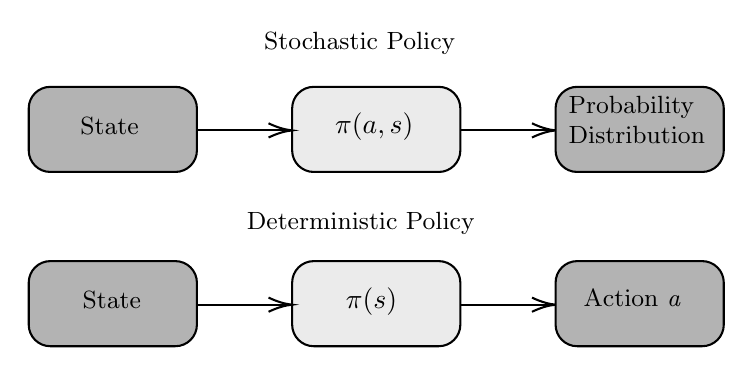
\begin{tikzpicture}[x=0.78pt,y=0.78pt,yscale=-1,xscale=1]
%uncomment if require: \path (0,300); %set diagram left start at 0, and has height of 300

%Shape: Rectangle [id:dp3593780300920657] 
\draw  [fill={rgb, 255:red, 179; green, 179; blue, 179 }  ,fill opacity=1 ] (159,108.35) .. controls (159,102.82) and (163.48,98.35) .. (169,98.35) -- (226.92,98.35) .. controls (232.44,98.35) and (236.92,102.82) .. (236.92,108.35) -- (236.92,127.78) .. controls (236.92,133.3) and (232.44,137.78) .. (226.92,137.78) -- (169,137.78) .. controls (163.48,137.78) and (159,133.3) .. (159,127.78) -- cycle ;
%Shape: Rectangle [id:dp8837468411891483] 
\draw  [fill={rgb, 255:red, 235; green, 235; blue, 235 }  ,fill opacity=1 ] (281.04,108.35) .. controls (281.04,102.82) and (285.52,98.35) .. (291.04,98.35) -- (348.96,98.35) .. controls (354.48,98.35) and (358.96,102.82) .. (358.96,108.35) -- (358.96,127.78) .. controls (358.96,133.3) and (354.48,137.78) .. (348.96,137.78) -- (291.04,137.78) .. controls (285.52,137.78) and (281.04,133.3) .. (281.04,127.78) -- cycle ;
%Straight Lines [id:da6295326376207329] 
\draw    (237.08,118.53) -- (279.04,118.53) ;
\draw [shift={(281.04,118.53)}, rotate = 180] [color={rgb, 255:red, 0; green, 0; blue, 0 }  ][line width=0.75]    (10.93,-3.29) .. controls (6.95,-1.4) and (3.31,-0.3) .. (0,0) .. controls (3.31,0.3) and (6.95,1.4) .. (10.93,3.29)   ;
%Straight Lines [id:da40547725689245295] 
\draw    (359.12,118.53) -- (401.08,118.53) ;
\draw [shift={(403.08,118.53)}, rotate = 180] [color={rgb, 255:red, 0; green, 0; blue, 0 }  ][line width=0.75]    (10.93,-3.29) .. controls (6.95,-1.4) and (3.31,-0.3) .. (0,0) .. controls (3.31,0.3) and (6.95,1.4) .. (10.93,3.29)   ;
%Shape: Rectangle [id:dp7201165423430957] 
\draw  [fill={rgb, 255:red, 179; green, 179; blue, 179 }  ,fill opacity=1 ] (403.08,108.35) .. controls (403.08,102.82) and (407.56,98.35) .. (413.08,98.35) -- (471,98.35) .. controls (476.52,98.35) and (481,102.82) .. (481,108.35) -- (481,127.78) .. controls (481,133.3) and (476.52,137.78) .. (471,137.78) -- (413.08,137.78) .. controls (407.56,137.78) and (403.08,133.3) .. (403.08,127.78) -- cycle ;
%Shape: Rectangle [id:dp4931791512397752] 
\draw  [fill={rgb, 255:red, 179; green, 179; blue, 179 }  ,fill opacity=1 ] (159,189.08) .. controls (159,183.56) and (163.48,179.08) .. (169,179.08) -- (226.92,179.08) .. controls (232.44,179.08) and (236.92,183.56) .. (236.92,189.08) -- (236.92,208.51) .. controls (236.92,214.03) and (232.44,218.51) .. (226.92,218.51) -- (169,218.51) .. controls (163.48,218.51) and (159,214.03) .. (159,208.51) -- cycle ;
%Shape: Rectangle [id:dp6384232571432122] 
\draw  [fill={rgb, 255:red, 235; green, 235; blue, 235 }  ,fill opacity=1 ] (281.04,189.08) .. controls (281.04,183.56) and (285.52,179.08) .. (291.04,179.08) -- (348.96,179.08) .. controls (354.48,179.08) and (358.96,183.56) .. (358.96,189.08) -- (358.96,208.51) .. controls (358.96,214.03) and (354.48,218.51) .. (348.96,218.51) -- (291.04,218.51) .. controls (285.52,218.51) and (281.04,214.03) .. (281.04,208.51) -- cycle ;
%Straight Lines [id:da7440480456403529] 
\draw    (237.08,199.27) -- (279.04,199.27) ;
\draw [shift={(281.04,199.27)}, rotate = 180] [color={rgb, 255:red, 0; green, 0; blue, 0 }  ][line width=0.75]    (10.93,-3.29) .. controls (6.95,-1.4) and (3.31,-0.3) .. (0,0) .. controls (3.31,0.3) and (6.95,1.4) .. (10.93,3.29)   ;
%Straight Lines [id:da8283889037686483] 
\draw    (359.12,199.27) -- (401.08,199.27) ;
\draw [shift={(403.08,199.27)}, rotate = 180] [color={rgb, 255:red, 0; green, 0; blue, 0 }  ][line width=0.75]    (10.93,-3.29) .. controls (6.95,-1.4) and (3.31,-0.3) .. (0,0) .. controls (3.31,0.3) and (6.95,1.4) .. (10.93,3.29)   ;
%Shape: Rectangle [id:dp07199829445547312] 
\draw  [fill={rgb, 255:red, 179; green, 179; blue, 179 }  ,fill opacity=1 ] (403.08,189.08) .. controls (403.08,183.56) and (407.56,179.08) .. (413.08,179.08) -- (471,179.08) .. controls (476.52,179.08) and (481,183.56) .. (481,189.08) -- (481,208.51) .. controls (481,214.03) and (476.52,218.51) .. (471,218.51) -- (413.08,218.51) .. controls (407.56,218.51) and (403.08,214.03) .. (403.08,208.51) -- cycle ;

% Text Node
\draw (181.53,111.03) node [anchor=north west][inner sep=0.75pt]  [font=\small] [align=left] {{\small State}};
% Text Node
\draw (299.53,109.03) node [anchor=north west][inner sep=0.75pt]    {$\pi (a,s)$};
% Text Node
\draw (407.68,101.06) node [anchor=north west][inner sep=0.75pt]  [font=\small] [align=left] {{\small Probability}\\{\small Distribution}};
% Text Node
\draw (182.53,191.77) node [anchor=north west][inner sep=0.75pt]  [font=\small] [align=left] {{\small State}};
% Text Node
\draw (304.5,189.77) node [anchor=north west][inner sep=0.75pt]    {$\pi ( s)$};
% Text Node
\draw (414.68,190.77) node [anchor=north west][inner sep=0.75pt]  [font=\small] [align=left] {Action \textit{a}};
% Text Node
\draw (266.61,71.42) node [anchor=north west][inner sep=0.75pt]  [font=\small] [align=left] {Stochastic Policy};
% Text Node
\draw (258.61,154.97) node [anchor=north west][inner sep=0.75pt]  [font=\small] [align=left] {Deterministic Policy};
\end{tikzpicture}
\caption{Comparison between deterministic and stochastic policies}
\label{deterministic}
\end{figure}

Next, the agent's model is a prediction of what the environment will do next, with $P$ the prediction of the next state and $R$ of the next reward:
 \begin{equation}
 	\begin{cases}
 		P_{s s^{'}}^{a}=\mathbb{P}[S_{t+1}=s^{'} \mid S_t = s, A_t = a ] \\
 		R_{s}^{a} = \mathbb{E} [ R_{t+1} \mid S_{t} = s, A_t = a ]
 	\end{cases}
 \end{equation}
 In the specific case of autonomous racing, it is quite challenging to implement a model-based algorithm because the ``rules" of a race are much more complicated to define than, for example, the rules of chess (\cite{modelbased}): we will thus mostly work with model-free methods. \newline
 Those concepts can be combined into a Markov Reward Process (Figure \ref{mrp}). It consists of a tuple $\left< S,P,R,\gamma \right>$ with:
 \begin{itemize}
 	\item $S$ a finite set of states
 	\item $P$ a state transition probability matrix ($P_{s s^{'}} = \mathbb{P} \left[ S_{t+1} = s^{'} \mid S_t = s \right]$
 	\item $R$ a reward function, $R_s = \mathbb{E} \left[ R_{t+1} \mid S_t = s \right]$ with $R: S \rightarrow \mathbb{R}$
 	\item $\gamma$ a discount factor, $\gamma \in [0,1]$
 \end{itemize}
 
 We are here using a very simplified example of a racing car going through a corner: this will be used as a running example in all sections.
 The MRP is expressing the idea of delayed reward: if the agent accelerates, it will receive more short-term reward but will get highly penalised when hitting the wall; we will now introduce functions to ``solve" this MRP by finding the path that gives the most reward. In this very simplified example, we consider that once the car has reached the state ``accelerate again", it can't accelerate any more and has to go to the state ``Hit wall". \newline
 The goal is to give a very general idea of how the RL controller of an autonomous racing car works; even though the actual algorithms we will implement on the F1Tenth platform are much more sophisticated, the idea is the same.
 
 \begin{figure}[H]
\centering
\tikzset{every picture/.style={line width=0.75pt}} %set default line width to 0.75pt        

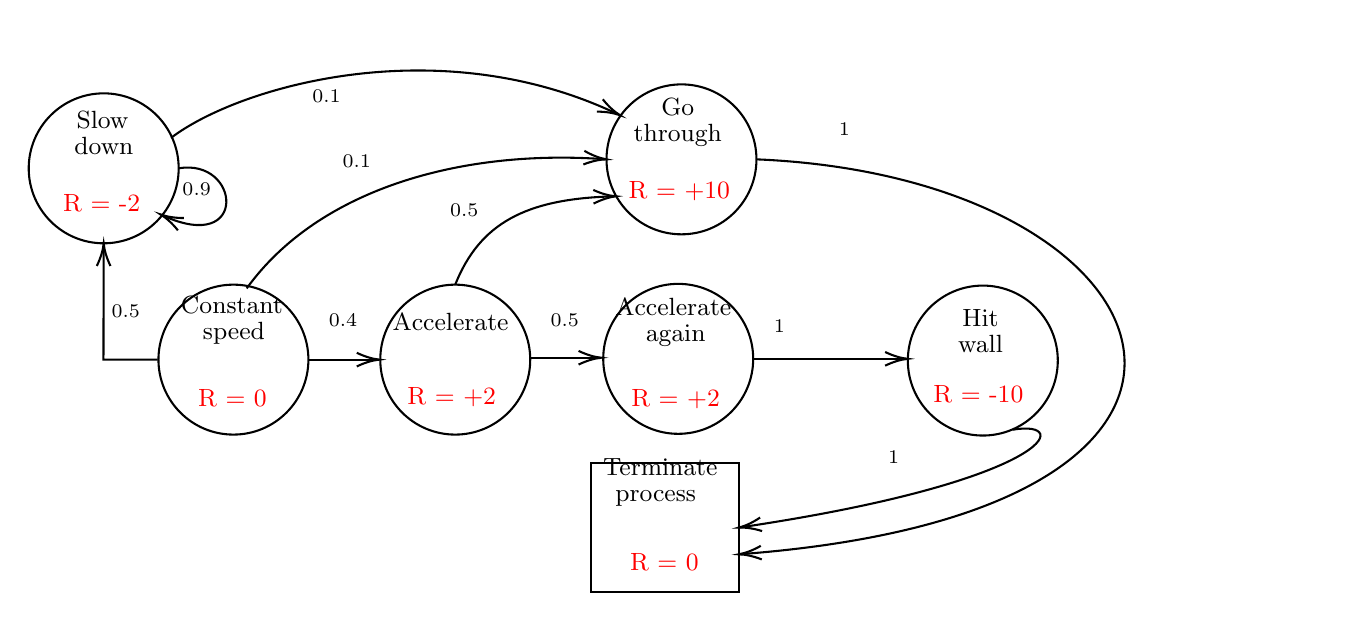
\begin{tikzpicture}[x=0.75pt,y=0.75pt,yscale=-1,xscale=1]
%uncomment if require: \path (0,300); %set diagram left start at 0, and has height of 300

%Shape: Rectangle [id:dp35173936232186764] 
\draw   (296,210.81) -- (367.12,210.81) -- (367.12,273) -- (296,273) -- cycle ;
%Shape: Ellipse [id:dp34773760147761856] 
\draw   (87.51,161.19) .. controls (87.51,141.24) and (103.68,125.07) .. (123.63,125.07) .. controls (143.58,125.07) and (159.75,141.24) .. (159.75,161.19) .. controls (159.75,181.14) and (143.58,197.31) .. (123.63,197.31) .. controls (103.68,197.31) and (87.51,181.14) .. (87.51,161.19) -- cycle ;
%Shape: Ellipse [id:dp6135239044961147] 
\draw   (25,69.03) .. controls (25,49.07) and (41.17,32.9) .. (61.12,32.9) .. controls (81.08,32.9) and (97.25,49.07) .. (97.25,69.03) .. controls (97.25,88.98) and (81.08,105.15) .. (61.12,105.15) .. controls (41.17,105.15) and (25,88.98) .. (25,69.03) -- cycle ;
%Shape: Ellipse [id:dp8428376855261868] 
\draw   (303.38,64.7) .. controls (303.38,44.75) and (319.55,28.58) .. (339.5,28.58) .. controls (359.45,28.58) and (375.62,44.75) .. (375.62,64.7) .. controls (375.62,84.65) and (359.45,100.82) .. (339.5,100.82) .. controls (319.55,100.82) and (303.38,84.65) .. (303.38,64.7) -- cycle ;
%Shape: Ellipse [id:dp40163172414467985] 
\draw   (301.8,160.81) .. controls (301.8,140.86) and (317.98,124.69) .. (337.93,124.69) .. controls (357.88,124.69) and (374.05,140.86) .. (374.05,160.81) .. controls (374.05,180.77) and (357.88,196.94) .. (337.93,196.94) .. controls (317.98,196.94) and (301.8,180.77) .. (301.8,160.81) -- cycle ;
%Shape: Ellipse [id:dp708288422656989] 
\draw   (448.56,161.64) .. controls (448.56,141.69) and (464.74,125.52) .. (484.69,125.52) .. controls (504.64,125.52) and (520.81,141.69) .. (520.81,161.64) .. controls (520.81,181.59) and (504.64,197.77) .. (484.69,197.77) .. controls (464.74,197.77) and (448.56,181.59) .. (448.56,161.64) -- cycle ;
%Curve Lines [id:da7085338027032924] 
\draw    (375.62,64.7) .. controls (580.57,73.2) and (644.88,234.41) .. (367.05,254.99) ;
\draw [shift={(367.05,254.99)}, rotate = 355.76] [color={rgb, 255:red, 0; green, 0; blue, 0 }  ][line width=0.75]    (10.93,-3.29) .. controls (6.95,-1.4) and (3.31,-0.3) .. (0,0) .. controls (3.31,0.3) and (6.95,1.4) .. (10.93,3.29)   ;
%Curve Lines [id:da33562544387773974] 
\draw    (499.1,194.97) .. controls (529.12,189.82) and (517.97,219.84) .. (367.05,242.13) ;
\draw [shift={(367.05,242.13)}, rotate = 351.6] [color={rgb, 255:red, 0; green, 0; blue, 0 }  ][line width=0.75]    (10.93,-3.29) .. controls (6.95,-1.4) and (3.31,-0.3) .. (0,0) .. controls (3.31,0.3) and (6.95,1.4) .. (10.93,3.29)   ;
%Straight Lines [id:da797455833484829] 
\draw    (374.05,160.81) -- (446.56,160.81) ;
\draw [shift={(448.56,160.81)}, rotate = 180] [color={rgb, 255:red, 0; green, 0; blue, 0 }  ][line width=0.75]    (10.93,-3.29) .. controls (6.95,-1.4) and (3.31,-0.3) .. (0,0) .. controls (3.31,0.3) and (6.95,1.4) .. (10.93,3.29)   ;
%Straight Lines [id:da6292687764035583] 
\draw    (159.75,161.19) -- (191.99,161.19) ;
\draw [shift={(193.99,161.19)}, rotate = 180] [color={rgb, 255:red, 0; green, 0; blue, 0 }  ][line width=0.75]    (10.93,-3.29) .. controls (6.95,-1.4) and (3.31,-0.3) .. (0,0) .. controls (3.31,0.3) and (6.95,1.4) .. (10.93,3.29)   ;
%Curve Lines [id:da8757855658609028] 
\draw    (97.25,69.03) .. controls (126.96,63.93) and (131.25,110.84) .. (89.73,91.81) ;
\draw [shift={(88.45,91.21)}, rotate = 25.64] [color={rgb, 255:red, 0; green, 0; blue, 0 }  ][line width=0.75]    (10.93,-3.29) .. controls (6.95,-1.4) and (3.31,-0.3) .. (0,0) .. controls (3.31,0.3) and (6.95,1.4) .. (10.93,3.29)   ;
%Curve Lines [id:da399738860785084] 
\draw    (93.6,54.34) .. controls (126.23,29.51) and (222.26,1.76) .. (308.7,42.87) ;
\draw [shift={(310,43.5)}, rotate = 205.84] [color={rgb, 255:red, 0; green, 0; blue, 0 }  ][line width=0.75]    (10.93,-3.29) .. controls (6.95,-1.4) and (3.31,-0.3) .. (0,0) .. controls (3.31,0.3) and (6.95,1.4) .. (10.93,3.29)   ;
%Straight Lines [id:da6623477064757914] 
\draw    (87.11,161.19) -- (61.01,161.19) -- (61.12,107.15) ;
\draw [shift={(61.12,105.15)}, rotate = 90.11] [color={rgb, 255:red, 0; green, 0; blue, 0 }  ][line width=0.75]    (10.93,-3.29) .. controls (6.95,-1.4) and (3.31,-0.3) .. (0,0) .. controls (3.31,0.3) and (6.95,1.4) .. (10.93,3.29)   ;
%Shape: Ellipse [id:dp6064442647048356] 
\draw   (194.38,161.19) .. controls (194.38,141.24) and (210.55,125.07) .. (230.5,125.07) .. controls (250.45,125.07) and (266.63,141.24) .. (266.63,161.19) .. controls (266.63,181.14) and (250.45,197.31) .. (230.5,197.31) .. controls (210.55,197.31) and (194.38,181.14) .. (194.38,161.19) -- cycle ;
%Straight Lines [id:da18265383373726918] 
\draw    (266.63,160.28) -- (298.86,160.28) ;
\draw [shift={(300.86,160.28)}, rotate = 180] [color={rgb, 255:red, 0; green, 0; blue, 0 }  ][line width=0.75]    (10.93,-3.29) .. controls (6.95,-1.4) and (3.31,-0.3) .. (0,0) .. controls (3.31,0.3) and (6.95,1.4) .. (10.93,3.29)   ;
%Curve Lines [id:da46424662234695435] 
\draw    (230.5,125.07) .. controls (242.22,95.6) and (264.39,83.77) .. (306.08,82.55) ;
\draw [shift={(308,82.5)}, rotate = 178.78] [color={rgb, 255:red, 0; green, 0; blue, 0 }  ][line width=0.75]    (10.93,-3.29) .. controls (6.95,-1.4) and (3.31,-0.3) .. (0,0) .. controls (3.31,0.3) and (6.95,1.4) .. (10.93,3.29)   ;
%Curve Lines [id:da6118717547111672] 
\draw    (130.02,126.89) .. controls (164.58,78.95) and (233.49,59.72) .. (302.34,64.62) ;
\draw [shift={(303.38,64.7)}, rotate = 184.28] [color={rgb, 255:red, 0; green, 0; blue, 0 }  ][line width=0.75]    (10.93,-3.29) .. controls (6.95,-1.4) and (3.31,-0.3) .. (0,0) .. controls (3.31,0.3) and (6.95,1.4) .. (10.93,3.29)   ;

% Text Node
\draw (45.54,39.8) node [anchor=north west][inner sep=0.75pt]  [font=\footnotesize] [align=left] {\begin{minipage}[lt]{20.28pt}\setlength\topsep{0pt}
\begin{center}
{\small Slow}\\{\small down}
\end{center}

\end{minipage}};
% Text Node
\draw (300.21,202.94) node [anchor=north west][inner sep=0.75pt]  [font=\footnotesize] [align=left] {\begin{minipage}[lt]{34.97pt}\setlength\topsep{0pt}
\begin{center}
{\small Terminate}\\{\small  \ process}
\end{center}

\end{minipage}};
% Text Node
\draw (309.87,33.93) node [anchor=north west][inner sep=0.75pt]  [font=\footnotesize] [align=left] {\begin{minipage}[lt]{39.47pt}\setlength\topsep{0pt}
\begin{center}
{\small Go through}
\end{center}

\end{minipage}};
% Text Node
\draw (96.87,124.73) node [anchor=north west][inner sep=0.75pt]  [font=\footnotesize] [align=left] {\begin{minipage}[lt]{32.11pt}\setlength\topsep{0pt}
\begin{center}
{\small Constant}\\{\small  \ \ speed}
\end{center}

\end{minipage}};
% Text Node
\draw (306.15,125.53) node [anchor=north west][inner sep=0.75pt]  [font=\footnotesize] [align=left] {\begin{minipage}[lt]{37.42pt}\setlength\topsep{0pt}
\begin{center}
{\small Accelerate}\\{\small  \ \ again}
\end{center}

\end{minipage}};
% Text Node
\draw (40.09,80.14) node [anchor=north west][inner sep=0.75pt]   [align=left] {{\small \textcolor[rgb]{1,0,0}{R = -2}}};
% Text Node
\draw (313.82,174.03) node [anchor=north west][inner sep=0.75pt]   [align=left] {{\small \textcolor[rgb]{1,0,0}{R = +2}}};
% Text Node
\draw (313.25,252.86) node [anchor=north west][inner sep=0.75pt]   [align=left] {{\small \textcolor[rgb]{1,0,0}{R = 0}}};
% Text Node
\draw (464.49,135.41) node [anchor=north west][inner sep=0.75pt]  [font=\footnotesize] [align=left] {\begin{minipage}[lt]{26.39pt}\setlength\topsep{0pt}
\begin{center}
{\small Hit wall}
\end{center}

\end{minipage}};
% Text Node
\draw (312.58,73.71) node [anchor=north west][inner sep=0.75pt]   [align=left] {{\small \textcolor[rgb]{1,0,0}{R = +10}}};
% Text Node
\draw (459.37,172.32) node [anchor=north west][inner sep=0.75pt]   [align=left] {{\small \textcolor[rgb]{1,0,0}{R = -10}}};
% Text Node
\draw (105.13,173.89) node [anchor=north west][inner sep=0.75pt]   [align=left] {{\small \textcolor[rgb]{1,0,0}{R = 0}}};
% Text Node
\draw (97.58,74.39) node [anchor=north west][inner sep=0.75pt]   [align=left] {{\scriptsize 0.9}};
% Text Node
\draw (160.14,29.72) node [anchor=north west][inner sep=0.75pt]   [align=left] {{\scriptsize 0.1}};
% Text Node
\draw (63.47,133.54) node [anchor=north west][inner sep=0.75pt]   [align=left] {{\scriptsize 0.5}};
% Text Node
\draw (168.06,137.66) node [anchor=north west][inner sep=0.75pt]   [align=left] {{\scriptsize 0.4}};
% Text Node
\draw (382.55,140.66) node [anchor=north west][inner sep=0.75pt]   [align=left] {{\scriptsize 1}};
% Text Node
\draw (437.59,203.64) node [anchor=north west][inner sep=0.75pt]   [align=left] {{\scriptsize 1}};
% Text Node
\draw (413.86,45.83) node [anchor=north west][inner sep=0.75pt]   [align=left] {{\scriptsize 1}};
% Text Node
\draw (198.83,133.03) node [anchor=north west][inner sep=0.75pt]  [font=\footnotesize] [align=left] {\begin{minipage}[lt]{37.42pt}\setlength\topsep{0pt}
\begin{center}
{\small Accelerate}
\end{center}

\end{minipage}};
% Text Node
\draw (206,172.89) node [anchor=north west][inner sep=0.75pt]   [align=left] {{\small \textcolor[rgb]{1,0,0}{R = +2}}};
% Text Node
\draw (274.93,137.66) node [anchor=north west][inner sep=0.75pt]   [align=left] {{\scriptsize 0.5}};
% Text Node
\draw (174.75,61.25) node [anchor=north west][inner sep=0.75pt]   [align=left] {{\scriptsize 0.1}};
% Text Node
\draw (226.52,84.68) node [anchor=north west][inner sep=0.75pt]   [align=left] {{\scriptsize 0.5}};


\end{tikzpicture}
\caption{Markov Reward Process Example}
\label{mrp}
\end{figure}

 A value function can then be defined as the total discounted reward of a policy starting in state $s$ (Equation \ref{valuefunction}):
\begin{equation}
\label{valuefunction}
	v_{\pi}(s)=\mathbb{E}_{\pi} \left[R_{t+1}+\gamma \: R_{t+2} + \gamma^{2} \:R_{t+3} + ... \mid S_t = s \right]
\end{equation}

 The discount factor $\gamma$ represents the compromise between short and long-term decision-making: $\gamma$ close to 0 will lead to a preference for short-term reward, whereas $\gamma$ close to 1 will lead to the opposite. Most MDPs are discounted, partly because the discount conveniently avoids infinite return in cyclic MDPs, although it is possible to use \textit{undiscounted} MDPs if all the sequences terminate. Furthermore, this is also closer to human and animal behaviour (preference for immediate reward), and it may be helpful if the reward is financial (more interest earned with immediate reward).\\
 We can then define the return $G_t$ as the total discounted reward from the time-step $t$ (\cite{silver2015}): 
 \begin{equation}
 	G_t = R_{t+1} + \gamma \: R_{t+2} + ... = \sum\limits_{k=0}^{\infty}\gamma^{k}R_{t+k+1}
 \end{equation}
 The value function of the MRP can then be defined as the expected return starting from state $s$:
 \begin{equation}
 \begin{split}
 	v(s) & = \mathbb{E}\left[G_t \mid S_t = s\right] \\
 	 & = \mathbb{E}\left[ R_{t+1} + \gamma \: v(S_{t+1}) \mid S_t= s \right]
 \end{split}
 \end{equation}
 
A MDP can now be defined as a MRP with $A$ added as a finite set of actions: $\left< S,A,P,R,\gamma \right>$ (\cite{mdpinai}). We will define a policy $\pi$ as a distribution over actions given states: $\pi(a \mid s) = \mathbb{P} [A_t = a \mid S_t = s]$. The state-value function $v_{\pi}(s)$ of an MDP is then the expected return starting from $s$ and following $\pi$. Similarly, the action-value function $q_{\pi}(s,a)= \mathbb{E}_{\pi}[G_t \mid S_t = s, A_t = a]$ is the expected return starting from $s$, doing $a$ and following $\pi$. Those two functions can again be decomposed as the sum of the immediate reward and the discounted value of the successor state (Equations \ref{svf} \ref{avf}):
 \begin{equation}
 \label{svf}
 	\begin{split}
 		v_\pi(s) & = \mathbb{E}_{\pi}[G_t \mid S_t = s] \\
 		& = \mathbb{E}_{\pi}[R_{t+1} + \gamma \: v_{\pi}(S_{t+1}) \mid S_t = s] \\
 		& = \sum\limits_{a \in A}\pi(a\mid
 		s) \: q_\pi(s,a) \\
 		& = \sum\limits_{a \in A}\pi(a \mid s)\left( R_s^{a} +\gamma \sum\limits_{s^{'} \in S} P_{ss^{'}}^{a}v_\pi(s^{'})\right)
 	\end{split}
 \end{equation}
 
 \begin{equation}
 \label{avf}
 	\begin{split}
 		q_{\pi}(s,a) & = \mathbb{E}_{\pi}[G_t \mid S_t = s, A_t = a] \\
 		& = \mathbb{E}_{\pi}[R_{t+1} + \gamma \: q_{\pi} (S_{t+1},A_{t+1}) \mid S_t = s, A_t = a ] \\
 		& = R_s^{a} + \gamma \sum\limits_{s^{'} \in S}P_{ss^{'}}^{a}v_\pi(s^{'}) \\
 		& = R_s^{a} + \gamma \sum\limits_{s^{'} \in S} P_{ss^{'}}^{a} \sum\limits_{a^{'} \in A}  \pi(a^{'} \mid s^{'})\: q_\pi(s^{'},a^{'})
 	\end{split}
 \end{equation}
Then, the optimal state-value function $v_*(s)= \underset{\pi}{max}\: v_\pi(s)$ and the optimal action-value function $q_*(s,a)=\underset{\pi}{max} \: q_\pi(s,a)$ can be defined respectively as the maximum value function and the maximum action-value function over all policies. They are represented in the example MDP Figures \ref{optimalvaluefunction} and \ref{optimalactionvaluefunction}.

\begin{figure}[H]
\centering



\tikzset{every picture/.style={line width=0.75pt}} %set default line width to 0.75pt        

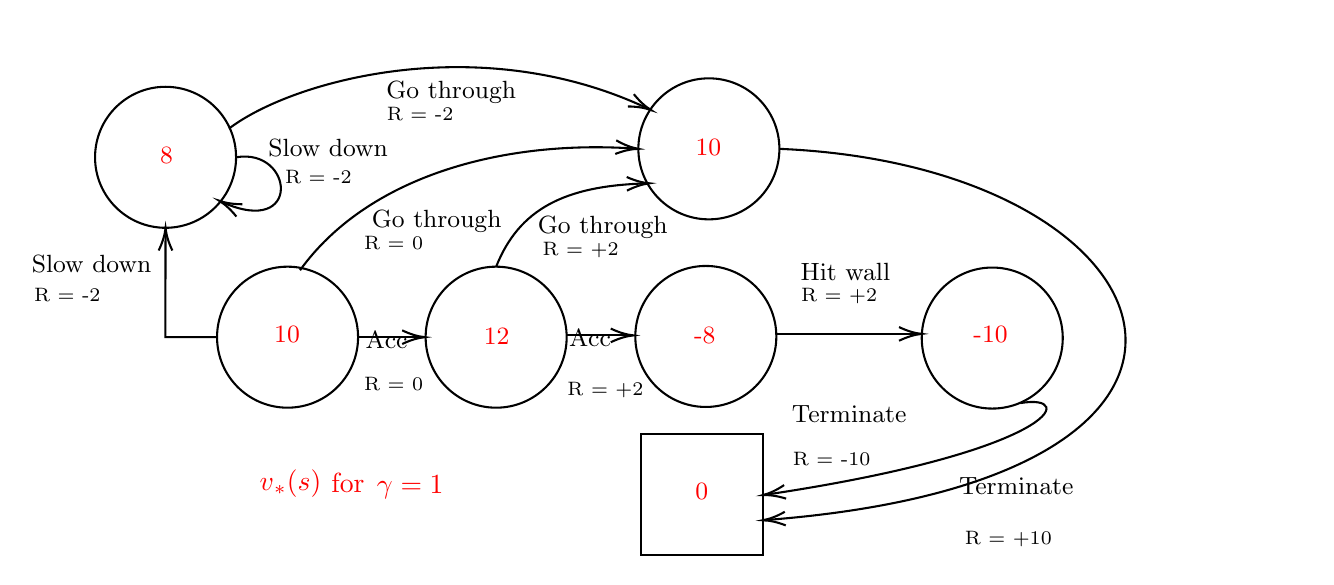
\begin{tikzpicture}[x=0.75pt,y=0.75pt,yscale=-1,xscale=1]
%uncomment if require: \path (0,300); %set diagram left start at 0, and has height of 300

%Shape: Rectangle [id:dp611059804808264] 
\draw   (308.23,191.52) -- (366.71,191.52) -- (366.71,250) -- (308.23,250) -- cycle ;
%Shape: Ellipse [id:dp08004009595563177] 
\draw   (103.78,144.86) .. controls (103.78,126.1) and (118.99,110.89) .. (137.75,110.89) .. controls (156.51,110.89) and (171.72,126.1) .. (171.72,144.86) .. controls (171.72,163.62) and (156.51,178.83) .. (137.75,178.83) .. controls (118.99,178.83) and (103.78,163.62) .. (103.78,144.86) -- cycle ;
%Shape: Ellipse [id:dp6391396725321665] 
\draw   (45,58.19) .. controls (45,39.43) and (60.21,24.22) .. (78.97,24.22) .. controls (97.73,24.22) and (112.94,39.43) .. (112.94,58.19) .. controls (112.94,76.95) and (97.73,92.16) .. (78.97,92.16) .. controls (60.21,92.16) and (45,76.95) .. (45,58.19) -- cycle ;
%Shape: Ellipse [id:dp9861716384017205] 
\draw   (306.77,54.12) .. controls (306.77,35.36) and (321.98,20.15) .. (340.74,20.15) .. controls (359.5,20.15) and (374.71,35.36) .. (374.71,54.12) .. controls (374.71,72.88) and (359.5,88.09) .. (340.74,88.09) .. controls (321.98,88.09) and (306.77,72.88) .. (306.77,54.12) -- cycle ;
%Shape: Ellipse [id:dp9319767586371086] 
\draw   (305.3,144.51) .. controls (305.3,125.74) and (320.5,110.54) .. (339.27,110.54) .. controls (358.03,110.54) and (373.24,125.74) .. (373.24,144.51) .. controls (373.24,163.27) and (358.03,178.48) .. (339.27,178.48) .. controls (320.5,178.48) and (305.3,163.27) .. (305.3,144.51) -- cycle ;
%Shape: Ellipse [id:dp5466793296229577] 
\draw   (443.3,145.28) .. controls (443.3,126.52) and (458.51,111.31) .. (477.27,111.31) .. controls (496.03,111.31) and (511.24,126.52) .. (511.24,145.28) .. controls (511.24,164.04) and (496.03,179.25) .. (477.27,179.25) .. controls (458.51,179.25) and (443.3,164.04) .. (443.3,145.28) -- cycle ;
%Curve Lines [id:da19355670591533003] 
\draw    (374.71,54.12) .. controls (567.43,62.12) and (627.91,213.71) .. (366.65,233.07) ;
\draw [shift={(366.65,233.07)}, rotate = 355.76] [color={rgb, 255:red, 0; green, 0; blue, 0 }  ][line width=0.75]    (10.93,-3.29) .. controls (6.95,-1.4) and (3.31,-0.3) .. (0,0) .. controls (3.31,0.3) and (6.95,1.4) .. (10.93,3.29)   ;
%Curve Lines [id:da9897958371381899] 
\draw    (490.83,176.62) .. controls (519.05,171.78) and (508.57,200.01) .. (366.65,220.97) ;
\draw [shift={(366.65,220.97)}, rotate = 351.6] [color={rgb, 255:red, 0; green, 0; blue, 0 }  ][line width=0.75]    (10.93,-3.29) .. controls (6.95,-1.4) and (3.31,-0.3) .. (0,0) .. controls (3.31,0.3) and (6.95,1.4) .. (10.93,3.29)   ;
%Straight Lines [id:da12057993663184008] 
\draw    (373.24,143.28) -- (441.3,143.28) ;
\draw [shift={(443.3,143.28)}, rotate = 180] [color={rgb, 255:red, 0; green, 0; blue, 0 }  ][line width=0.75]    (10.93,-3.29) .. controls (6.95,-1.4) and (3.31,-0.3) .. (0,0) .. controls (3.31,0.3) and (6.95,1.4) .. (10.93,3.29)   ;
%Straight Lines [id:da23951457390958297] 
\draw    (171.72,144.86) -- (201.91,144.86) ;
\draw [shift={(203.91,144.86)}, rotate = 180] [color={rgb, 255:red, 0; green, 0; blue, 0 }  ][line width=0.75]    (10.93,-3.29) .. controls (6.95,-1.4) and (3.31,-0.3) .. (0,0) .. controls (3.31,0.3) and (6.95,1.4) .. (10.93,3.29)   ;
%Curve Lines [id:da5265057856586608] 
\draw    (112.94,58.19) .. controls (140.74,53.42) and (144.87,97.06) .. (106.45,79.88) ;
\draw [shift={(104.67,79.05)}, rotate = 25.64] [color={rgb, 255:red, 0; green, 0; blue, 0 }  ][line width=0.75]    (10.93,-3.29) .. controls (6.95,-1.4) and (3.31,-0.3) .. (0,0) .. controls (3.31,0.3) and (6.95,1.4) .. (10.93,3.29)   ;
%Curve Lines [id:da8028340889706267] 
\draw    (109.51,44.38) .. controls (140.19,21.03) and (230.49,-3.76) .. (311.78,34.91) ;
\draw [shift={(313,35.5)}, rotate = 205.84] [color={rgb, 255:red, 0; green, 0; blue, 0 }  ][line width=0.75]    (10.93,-3.29) .. controls (6.95,-1.4) and (3.31,-0.3) .. (0,0) .. controls (3.31,0.3) and (6.95,1.4) .. (10.93,3.29)   ;
%Straight Lines [id:da1700393412175667] 
\draw    (103.41,144.86) -- (78.87,144.86) -- (78.97,94.16) ;
\draw [shift={(78.97,92.16)}, rotate = 90.11] [color={rgb, 255:red, 0; green, 0; blue, 0 }  ][line width=0.75]    (10.93,-3.29) .. controls (6.95,-1.4) and (3.31,-0.3) .. (0,0) .. controls (3.31,0.3) and (6.95,1.4) .. (10.93,3.29)   ;
%Shape: Ellipse [id:dp14942833793184196] 
\draw   (204.28,144.86) .. controls (204.28,126.1) and (219.49,110.89) .. (238.25,110.89) .. controls (257.01,110.89) and (272.22,126.1) .. (272.22,144.86) .. controls (272.22,163.62) and (257.01,178.83) .. (238.25,178.83) .. controls (219.49,178.83) and (204.28,163.62) .. (204.28,144.86) -- cycle ;
%Straight Lines [id:da43732456965491484] 
\draw    (272.22,144) -- (302.41,144) ;
\draw [shift={(304.41,144)}, rotate = 180] [color={rgb, 255:red, 0; green, 0; blue, 0 }  ][line width=0.75]    (10.93,-3.29) .. controls (6.95,-1.4) and (3.31,-0.3) .. (0,0) .. controls (3.31,0.3) and (6.95,1.4) .. (10.93,3.29)   ;
%Curve Lines [id:da7695240440294568] 
\draw    (238.25,110.89) .. controls (249.27,83.18) and (271.1,71.93) .. (310.34,70.78) ;
\draw [shift={(312.14,70.73)}, rotate = 178.78] [color={rgb, 255:red, 0; green, 0; blue, 0 }  ][line width=0.75]    (10.93,-3.29) .. controls (6.95,-1.4) and (3.31,-0.3) .. (0,0) .. controls (3.31,0.3) and (6.95,1.4) .. (10.93,3.29)   ;
%Curve Lines [id:da3564367220755964] 
\draw    (143.76,112.61) .. controls (176.1,67.75) and (240.4,49.62) .. (304.82,53.98) ;
\draw [shift={(306.77,54.12)}, rotate = 184.28] [color={rgb, 255:red, 0; green, 0; blue, 0 }  ][line width=0.75]    (10.93,-3.29) .. controls (6.95,-1.4) and (3.31,-0.3) .. (0,0) .. controls (3.31,0.3) and (6.95,1.4) .. (10.93,3.29)   ;

% Text Node
\draw (127.04,47.75) node [anchor=north west][inner sep=0.75pt]  [font=\footnotesize] [align=left] {{\small Slow down}};
% Text Node
\draw (383.44,107.72) node [anchor=north west][inner sep=0.75pt]  [font=\footnotesize] [align=left] {{\small Hit wall \ }};
% Text Node
\draw (135.12,62.8) node [anchor=north west][inner sep=0.75pt]   [align=left] {{\scriptsize \textcolor[rgb]{0,0,0}{R = -2}}};
% Text Node
\draw (332.14,138.78) node [anchor=north west][inner sep=0.75pt]   [align=left] {{\small \textcolor[rgb]{1,0,0}{-8}}};
% Text Node
\draw (332.72,213.79) node [anchor=north west][inner sep=0.75pt]   [align=left] {{\small \textcolor[rgb]{1,0,0}{0}}};
% Text Node
\draw (379.27,171.75) node [anchor=north west][inner sep=0.75pt]  [font=\footnotesize] [align=left] {\begin{minipage}[lt]{34.97pt}\setlength\topsep{0pt}
\begin{center}
{\small Terminate}
\end{center}

\end{minipage}};
% Text Node
\draw (332.82,48.09) node [anchor=north west][inner sep=0.75pt]   [align=left] {{\small \textcolor[rgb]{1,0,0}{10}}};
% Text Node
\draw (466.73,138.31) node [anchor=north west][inner sep=0.75pt]   [align=left] {\textcolor[rgb]{1,0,0}{{\small -10}}};
% Text Node
\draw (122.81,207.33) node [anchor=north west][inner sep=0.75pt]    {$\textcolor[rgb]{1,0,0}{v}\textcolor[rgb]{1,0,0}{_{*}}\textcolor[rgb]{1,0,0}{(}\textcolor[rgb]{1,0,0}{s}\textcolor[rgb]{1,0,0}{)}$};
% Text Node
\draw (157.36,209.14) node [anchor=north west][inner sep=0.75pt]   [align=left] {\textcolor[rgb]{1,0,0}{for}};
% Text Node
\draw (179.32,210.1) node [anchor=north west][inner sep=0.75pt]    {$\textcolor[rgb]{1,0,0}{\gamma = 1}$};
% Text Node
\draw (459.76,206.53) node [anchor=north west][inner sep=0.75pt]  [font=\footnotesize] [align=left] {\begin{minipage}[lt]{34.97pt}\setlength\topsep{0pt}
\begin{center}
{\small Terminate}
\end{center}

\end{minipage}};
% Text Node
\draw (462.54,236.71) node [anchor=north west][inner sep=0.75pt]   [align=left] {{\scriptsize \textcolor[rgb]{0,0,0}{R = +10}}};
% Text Node
\draw (379.73,198.87) node [anchor=north west][inner sep=0.75pt]   [align=left] {{\scriptsize \textcolor[rgb]{0,0,0}{R = -10}}};
% Text Node
\draw (383.73,119.87) node [anchor=north west][inner sep=0.75pt]   [align=left] {{\scriptsize \textcolor[rgb]{0,0,0}{R = +2}}};
% Text Node
\draw (183.87,19.93) node [anchor=north west][inner sep=0.75pt]  [font=\footnotesize] [align=left] {{\small Go through}};
% Text Node
\draw (184.12,32.8) node [anchor=north west][inner sep=0.75pt]   [align=left] {{\scriptsize \textcolor[rgb]{0,0,0}{R = -2}}};
% Text Node
\draw (176.87,82) node [anchor=north west][inner sep=0.75pt]  [font=\footnotesize] [align=left] {{\small Go through }};
% Text Node
\draw (173.12,94.87) node [anchor=north west][inner sep=0.75pt]   [align=left] {{\scriptsize \textcolor[rgb]{0,0,0}{R = 0}}};
% Text Node
\draw (256.87,85) node [anchor=north west][inner sep=0.75pt]  [font=\footnotesize] [align=left] {{\small Go through }};
% Text Node
\draw (259.12,97.87) node [anchor=north west][inner sep=0.75pt]   [align=left] {{\scriptsize \textcolor[rgb]{0,0,0}{R = +2}}};
% Text Node
\draw (271.87,135) node [anchor=north west][inner sep=0.75pt]  [font=\footnotesize] [align=left] {\begin{minipage}[lt]{14.97pt}\setlength\topsep{0pt}
\begin{center}
{\small Acc}
\end{center}

\end{minipage}};
% Text Node
\draw (173.87,136) node [anchor=north west][inner sep=0.75pt]  [font=\footnotesize] [align=left] {\begin{minipage}[lt]{14.97pt}\setlength\topsep{0pt}
\begin{center}
{\small Acc}
\end{center}

\end{minipage}};
% Text Node
\draw (230.82,139.09) node [anchor=north west][inner sep=0.75pt]   [align=left] {{\small \textcolor[rgb]{1,0,0}{12}}};
% Text Node
\draw (271.12,164.87) node [anchor=north west][inner sep=0.75pt]   [align=left] {{\scriptsize \textcolor[rgb]{0,0,0}{R = +2}}};
% Text Node
\draw (173.12,162.87) node [anchor=north west][inner sep=0.75pt]   [align=left] {{\scriptsize \textcolor[rgb]{0,0,0}{R = 0}}};
% Text Node
\draw (14.12,119.87) node [anchor=north west][inner sep=0.75pt]   [align=left] {{\scriptsize \textcolor[rgb]{0,0,0}{R = -2}}};
% Text Node
\draw (13.04,103.75) node [anchor=north west][inner sep=0.75pt]  [font=\footnotesize] [align=left] {{\small Slow down}};
% Text Node
\draw (129.82,138.09) node [anchor=north west][inner sep=0.75pt]   [align=left] {{\small \textcolor[rgb]{1,0,0}{10}}};
% Text Node
\draw (74.82,52.09) node [anchor=north west][inner sep=0.75pt]   [align=left] {{\small \textcolor[rgb]{1,0,0}{8}}};


\end{tikzpicture}
\caption{Optimal Value Function of an MDP}
\label{optimalvaluefunction}
\end{figure}

The values in red are $v_*(s)$ calculated with $\gamma = 1$. They represent the best value the agent can get from the MDP when starting in state $s$.

\begin{figure}[H]
\centering



\tikzset{every picture/.style={line width=0.75pt}} %set default line width to 0.75pt        

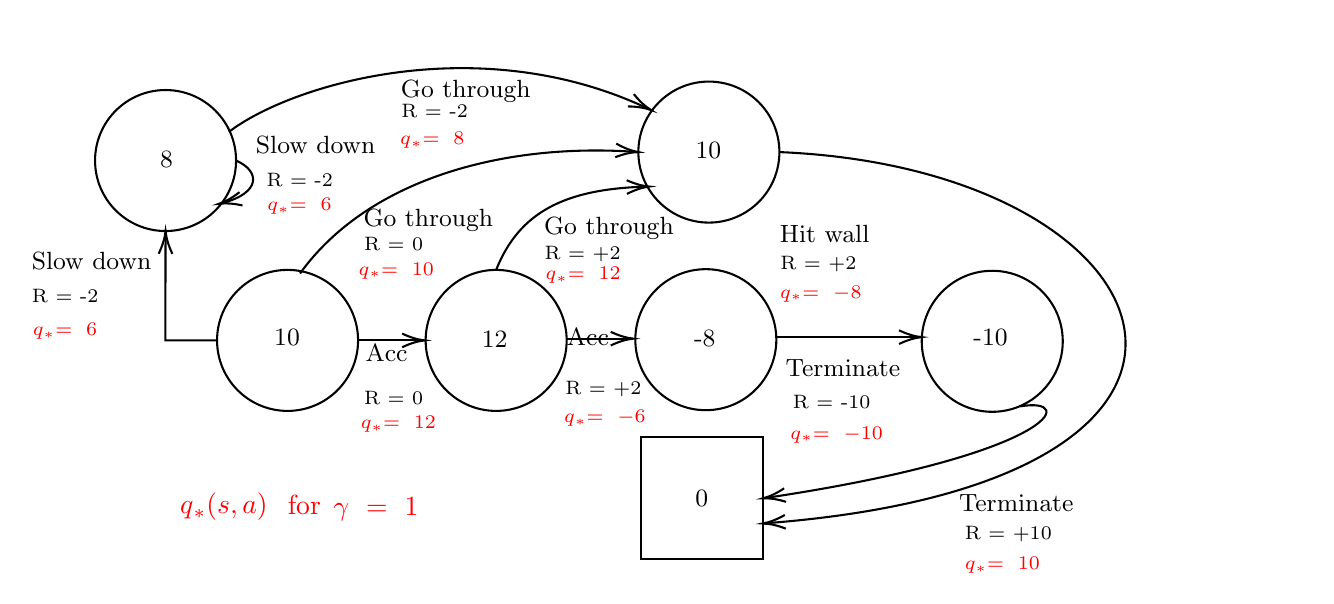
\begin{tikzpicture}[x=0.75pt,y=0.75pt,yscale=-1,xscale=1]
%uncomment if require: \path (0,300); %set diagram left start at 0, and has height of 300

%Shape: Rectangle [id:dp7996894340412215] 
\draw   (328.23,216.58) -- (386.71,216.58) -- (386.71,275.07) -- (328.23,275.07) -- cycle ;
%Shape: Ellipse [id:dp9238263655797876] 
\draw   (123.78,169.92) .. controls (123.78,151.16) and (138.99,135.95) .. (157.75,135.95) .. controls (176.51,135.95) and (191.72,151.16) .. (191.72,169.92) .. controls (191.72,188.69) and (176.51,203.89) .. (157.75,203.89) .. controls (138.99,203.89) and (123.78,188.69) .. (123.78,169.92) -- cycle ;
%Shape: Ellipse [id:dp00077189549681278] 
\draw   (65,83.26) .. controls (65,64.49) and (80.21,49.29) .. (98.97,49.29) .. controls (117.73,49.29) and (132.94,64.49) .. (132.94,83.26) .. controls (132.94,102.02) and (117.73,117.23) .. (98.97,117.23) .. controls (80.21,117.23) and (65,102.02) .. (65,83.26) -- cycle ;
%Shape: Ellipse [id:dp19539664605782736] 
\draw   (326.77,79.19) .. controls (326.77,60.43) and (341.98,45.22) .. (360.74,45.22) .. controls (379.5,45.22) and (394.71,60.43) .. (394.71,79.19) .. controls (394.71,97.95) and (379.5,113.16) .. (360.74,113.16) .. controls (341.98,113.16) and (326.77,97.95) .. (326.77,79.19) -- cycle ;
%Shape: Ellipse [id:dp989045239528632] 
\draw   (325.3,169.57) .. controls (325.3,150.81) and (340.5,135.6) .. (359.27,135.6) .. controls (378.03,135.6) and (393.24,150.81) .. (393.24,169.57) .. controls (393.24,188.33) and (378.03,203.54) .. (359.27,203.54) .. controls (340.5,203.54) and (325.3,188.33) .. (325.3,169.57) -- cycle ;
%Shape: Ellipse [id:dp7266051122955972] 
\draw   (463.3,170.35) .. controls (463.3,151.59) and (478.51,136.38) .. (497.27,136.38) .. controls (516.03,136.38) and (531.24,151.59) .. (531.24,170.35) .. controls (531.24,189.11) and (516.03,204.32) .. (497.27,204.32) .. controls (478.51,204.32) and (463.3,189.11) .. (463.3,170.35) -- cycle ;
%Curve Lines [id:da8411018328671096] 
\draw    (394.71,79.19) .. controls (587.43,87.18) and (647.91,238.78) .. (386.65,258.13) ;
\draw [shift={(386.65,258.13)}, rotate = 355.76] [color={rgb, 255:red, 0; green, 0; blue, 0 }  ][line width=0.75]    (10.93,-3.29) .. controls (6.95,-1.4) and (3.31,-0.3) .. (0,0) .. controls (3.31,0.3) and (6.95,1.4) .. (10.93,3.29)   ;
%Curve Lines [id:da32919886386468367] 
\draw    (510.83,201.69) .. controls (539.05,196.85) and (528.57,225.07) .. (386.65,246.04) ;
\draw [shift={(386.65,246.04)}, rotate = 351.6] [color={rgb, 255:red, 0; green, 0; blue, 0 }  ][line width=0.75]    (10.93,-3.29) .. controls (6.95,-1.4) and (3.31,-0.3) .. (0,0) .. controls (3.31,0.3) and (6.95,1.4) .. (10.93,3.29)   ;
%Straight Lines [id:da23236521724922254] 
\draw    (393.24,168.35) -- (461.3,168.35) ;
\draw [shift={(463.3,168.35)}, rotate = 180] [color={rgb, 255:red, 0; green, 0; blue, 0 }  ][line width=0.75]    (10.93,-3.29) .. controls (6.95,-1.4) and (3.31,-0.3) .. (0,0) .. controls (3.31,0.3) and (6.95,1.4) .. (10.93,3.29)   ;
%Straight Lines [id:da8481335296043679] 
\draw    (191.72,169.92) -- (221.91,169.92) ;
\draw [shift={(223.91,169.92)}, rotate = 180] [color={rgb, 255:red, 0; green, 0; blue, 0 }  ][line width=0.75]    (10.93,-3.29) .. controls (6.95,-1.4) and (3.31,-0.3) .. (0,0) .. controls (3.31,0.3) and (6.95,1.4) .. (10.93,3.29)   ;
%Curve Lines [id:da3339550155750177] 
\draw    (132.94,83.26) .. controls (144.64,88.34) and (144.99,98.85) .. (126.45,103.69) ;
\draw [shift={(124.67,104.12)}, rotate = 347.2] [color={rgb, 255:red, 0; green, 0; blue, 0 }  ][line width=0.75]    (10.93,-3.29) .. controls (6.95,-1.4) and (3.31,-0.3) .. (0,0) .. controls (3.31,0.3) and (6.95,1.4) .. (10.93,3.29)   ;
%Curve Lines [id:da599882851327479] 
\draw    (129.51,69.44) .. controls (160.19,46.09) and (250.49,19.75) .. (331.78,58.41) ;
\draw [shift={(333,59)}, rotate = 205.84] [color={rgb, 255:red, 0; green, 0; blue, 0 }  ][line width=0.75]    (10.93,-3.29) .. controls (6.95,-1.4) and (3.31,-0.3) .. (0,0) .. controls (3.31,0.3) and (6.95,1.4) .. (10.93,3.29)   ;
%Straight Lines [id:da2133400414366724] 
\draw    (123.41,169.92) -- (98.87,169.92) -- (98.97,119.23) ;
\draw [shift={(98.97,117.23)}, rotate = 90.11] [color={rgb, 255:red, 0; green, 0; blue, 0 }  ][line width=0.75]    (10.93,-3.29) .. controls (6.95,-1.4) and (3.31,-0.3) .. (0,0) .. controls (3.31,0.3) and (6.95,1.4) .. (10.93,3.29)   ;
%Shape: Ellipse [id:dp33060312070062725] 
\draw   (224.28,169.92) .. controls (224.28,151.16) and (239.49,135.95) .. (258.25,135.95) .. controls (277.01,135.95) and (292.22,151.16) .. (292.22,169.92) .. controls (292.22,188.69) and (277.01,203.89) .. (258.25,203.89) .. controls (239.49,203.89) and (224.28,188.69) .. (224.28,169.92) -- cycle ;
%Straight Lines [id:da0942296358412873] 
\draw    (292.22,169.07) -- (322.41,169.07) ;
\draw [shift={(324.41,169.07)}, rotate = 180] [color={rgb, 255:red, 0; green, 0; blue, 0 }  ][line width=0.75]    (10.93,-3.29) .. controls (6.95,-1.4) and (3.31,-0.3) .. (0,0) .. controls (3.31,0.3) and (6.95,1.4) .. (10.93,3.29)   ;
%Curve Lines [id:da31598187812982825] 
\draw    (258.25,135.95) .. controls (269.27,108.24) and (291.1,96.99) .. (330.34,95.84) ;
\draw [shift={(332.14,95.8)}, rotate = 178.78] [color={rgb, 255:red, 0; green, 0; blue, 0 }  ][line width=0.75]    (10.93,-3.29) .. controls (6.95,-1.4) and (3.31,-0.3) .. (0,0) .. controls (3.31,0.3) and (6.95,1.4) .. (10.93,3.29)   ;
%Curve Lines [id:da9694062102653032] 
\draw    (163.76,137.67) .. controls (196.1,92.81) and (260.4,74.69) .. (324.82,79.05) ;
\draw [shift={(326.77,79.19)}, rotate = 184.28] [color={rgb, 255:red, 0; green, 0; blue, 0 }  ][line width=0.75]    (10.93,-3.29) .. controls (6.95,-1.4) and (3.31,-0.3) .. (0,0) .. controls (3.31,0.3) and (6.95,1.4) .. (10.93,3.29)   ;

% Text Node
\draw (141.04,69.81) node [anchor=north west][inner sep=0.75pt]  [font=\footnotesize] [align=left] {{\small Slow down}};
% Text Node
\draw (393.44,112.78) node [anchor=north west][inner sep=0.75pt]  [font=\footnotesize] [align=left] {{\small Hit wall}};
% Text Node
\draw (146.12,87.87) node [anchor=north west][inner sep=0.75pt]   [align=left] {{\scriptsize \textcolor[rgb]{0,0,0}{R = -2}}};
% Text Node
\draw (352.14,163.85) node [anchor=north west][inner sep=0.75pt]   [align=left] {{\small \textcolor[rgb]{0,0,0}{-8}}};
% Text Node
\draw (352.72,240.86) node [anchor=north west][inner sep=0.75pt]   [align=left] {{\small \textcolor[rgb]{0,0,0}{0}}};
% Text Node
\draw (396.27,177.81) node [anchor=north west][inner sep=0.75pt]  [font=\footnotesize] [align=left] {{\small Terminate}};
% Text Node
\draw (352.82,73.15) node [anchor=north west][inner sep=0.75pt]   [align=left] {{\small \textcolor[rgb]{0,0,0}{10}}};
% Text Node
\draw (486.73,163.38) node [anchor=north west][inner sep=0.75pt]   [align=left] {\textcolor[rgb]{0,0,0}{{\small -10}}};
% Text Node
\draw (156.36,243.2) node [anchor=north west][inner sep=0.75pt]   [align=left] {\textcolor[rgb]{1,0,0}{for}};
% Text Node
\draw (178.32,244.17) node [anchor=north west][inner sep=0.75pt]    {$\textcolor[rgb]{1,0,0}{\gamma\ =\ 1}$};
% Text Node
\draw (479.76,242.59) node [anchor=north west][inner sep=0.75pt]  [font=\footnotesize] [align=left] {{\small Terminate}};
% Text Node
\draw (482.54,257.78) node [anchor=north west][inner sep=0.75pt]   [align=left] {{\scriptsize \textcolor[rgb]{0,0,0}{R = +10}}};
% Text Node
\draw (399.73,194.94) node [anchor=north west][inner sep=0.75pt]   [align=left] {{\scriptsize \textcolor[rgb]{0,0,0}{R = -10}}};
% Text Node
\draw (393.73,127.94) node [anchor=north west][inner sep=0.75pt]   [align=left] {{\scriptsize \textcolor[rgb]{0,0,0}{R = +2}}};
% Text Node
\draw (210.87,43) node [anchor=north west][inner sep=0.75pt]  [font=\footnotesize] [align=left] {{\small Go through}};
% Text Node
\draw (211.12,54.87) node [anchor=north west][inner sep=0.75pt]   [align=left] {{\scriptsize \textcolor[rgb]{0,0,0}{R = -2}}};
% Text Node
\draw (192.87,105.07) node [anchor=north west][inner sep=0.75pt]  [font=\footnotesize] [align=left] {{\small Go through}};
% Text Node
\draw (193.12,118.93) node [anchor=north west][inner sep=0.75pt]   [align=left] {{\scriptsize \textcolor[rgb]{0,0,0}{R = 0}}};
% Text Node
\draw (279.87,109.07) node [anchor=north west][inner sep=0.75pt]  [font=\footnotesize] [align=left] {{\small Go through}};
% Text Node
\draw (280.12,122.93) node [anchor=north west][inner sep=0.75pt]   [align=left] {{\scriptsize \textcolor[rgb]{0,0,0}{R = +2}}};
% Text Node
\draw (290.87,158.07) node [anchor=north west][inner sep=0.75pt]  [font=\footnotesize] [align=left] {\begin{minipage}[lt]{14.97pt}\setlength\topsep{0pt}
\begin{center}
{\small Acc}
\end{center}

\end{minipage}};
% Text Node
\draw (193.87,166.07) node [anchor=north west][inner sep=0.75pt]  [font=\footnotesize] [align=left] {\begin{minipage}[lt]{14.97pt}\setlength\topsep{0pt}
\begin{center}
{\small Acc}
\end{center}

\end{minipage}};
% Text Node
\draw (249.82,164.15) node [anchor=north west][inner sep=0.75pt]   [align=left] {{\small \textcolor[rgb]{0,0,0}{12}}};
% Text Node
\draw (290.12,187.93) node [anchor=north west][inner sep=0.75pt]   [align=left] {{\scriptsize \textcolor[rgb]{0,0,0}{R = +2}}};
% Text Node
\draw (193.12,192.93) node [anchor=north west][inner sep=0.75pt]   [align=left] {{\scriptsize \textcolor[rgb]{0,0,0}{R = 0}}};
% Text Node
\draw (33.12,143.93) node [anchor=north west][inner sep=0.75pt]   [align=left] {{\scriptsize \textcolor[rgb]{0,0,0}{R = -2}}};
% Text Node
\draw (33.04,125.81) node [anchor=north west][inner sep=0.75pt]  [font=\footnotesize] [align=left] {{\small Slow down}};
% Text Node
\draw (149.82,163.15) node [anchor=north west][inner sep=0.75pt]   [align=left] {{\small \textcolor[rgb]{0,0,0}{10}}};
% Text Node
\draw (94.82,77.15) node [anchor=north west][inner sep=0.75pt]   [align=left] {{\small \textcolor[rgb]{0,0,0}{8}}};
% Text Node
\draw (104.54,242) node [anchor=north west][inner sep=0.75pt]    {$\textcolor[rgb]{1,0,0}{q}\textcolor[rgb]{1,0,0}{_{*}}\textcolor[rgb]{1,0,0}{(}\textcolor[rgb]{1,0,0}{s,a}\textcolor[rgb]{1,0,0}{)}$};
% Text Node
\draw (393.54,142) node [anchor=north west][inner sep=0.75pt]  [font=\scriptsize]  {${\textstyle \textcolor[rgb]{1,0,0}{q}\textcolor[rgb]{1,0,0}{_{*}}\textcolor[rgb]{1,0,0}{=\ -8}}$};
% Text Node
\draw (398.54,210) node [anchor=north west][inner sep=0.75pt]  [font=\scriptsize]  {${\textstyle \textcolor[rgb]{1,0,0}{q}\textcolor[rgb]{1,0,0}{_{*}}\textcolor[rgb]{1,0,0}{=\ -10}}$};
% Text Node
\draw (482.54,273) node [anchor=north west][inner sep=0.75pt]  [font=\scriptsize]  {${\textstyle \textcolor[rgb]{1,0,0}{q}\textcolor[rgb]{1,0,0}{_{*}}\textcolor[rgb]{1,0,0}{=\ 10}}$};
% Text Node
\draw (289.54,202) node [anchor=north west][inner sep=0.75pt]  [font=\scriptsize]  {${\textstyle \textcolor[rgb]{1,0,0}{q}\textcolor[rgb]{1,0,0}{_{*}}\textcolor[rgb]{1,0,0}{=\ -6}}$};
% Text Node
\draw (191.54,205) node [anchor=north west][inner sep=0.75pt]  [font=\scriptsize]  {${\textstyle \textcolor[rgb]{1,0,0}{q}\textcolor[rgb]{1,0,0}{_{*}}\textcolor[rgb]{1,0,0}{=\ 12}}$};
% Text Node
\draw (190.54,131) node [anchor=north west][inner sep=0.75pt]  [font=\scriptsize]  {${\textstyle \textcolor[rgb]{1,0,0}{q}\textcolor[rgb]{1,0,0}{_{*}}\textcolor[rgb]{1,0,0}{=\ 10}}$};
% Text Node
\draw (280.54,133) node [anchor=north west][inner sep=0.75pt]  [font=\scriptsize]  {${\textstyle \textcolor[rgb]{1,0,0}{q}\textcolor[rgb]{1,0,0}{_{*}}\textcolor[rgb]{1,0,0}{=\ 12}}$};
% Text Node
\draw (210.54,68) node [anchor=north west][inner sep=0.75pt]  [font=\scriptsize]  {${\textstyle \textcolor[rgb]{1,0,0}{q}\textcolor[rgb]{1,0,0}{_{*}}\textcolor[rgb]{1,0,0}{=\ 8}}$};
% Text Node
\draw (146.54,100) node [anchor=north west][inner sep=0.75pt]  [font=\scriptsize]  {${\textstyle \textcolor[rgb]{1,0,0}{q}\textcolor[rgb]{1,0,0}{_{*}}\textcolor[rgb]{1,0,0}{=\ 6}}$};
% Text Node
\draw (33.54,160) node [anchor=north west][inner sep=0.75pt]  [font=\scriptsize]  {${\textstyle \textcolor[rgb]{1,0,0}{q}\textcolor[rgb]{1,0,0}{_{*}}\textcolor[rgb]{1,0,0}{=\ 6}}$};


\end{tikzpicture}
\caption{Optimal Action-Value Function of an MDP}
\label{optimalactionvaluefunction}
\end{figure}


 The goal of an RL algorithm is to find the best approximate of $q_*(s,a)$ to solve the MDP. Once $q_*(s,a)$ is known, the optimal policy $\pi_* \geq \pi, \forall \pi$ ($\pi \geq \pi^{'}$ if $v_\pi(s) \geq v_{\pi^{'}}(s), \forall s$) can be found by maximising over $q_*(s,a)$, as can be seen in Figure \ref{optimalpolicymdp}.
 
 \begin{figure}[H]
\centering



\tikzset{every picture/.style={line width=0.75pt}} %set default line width to 0.75pt        

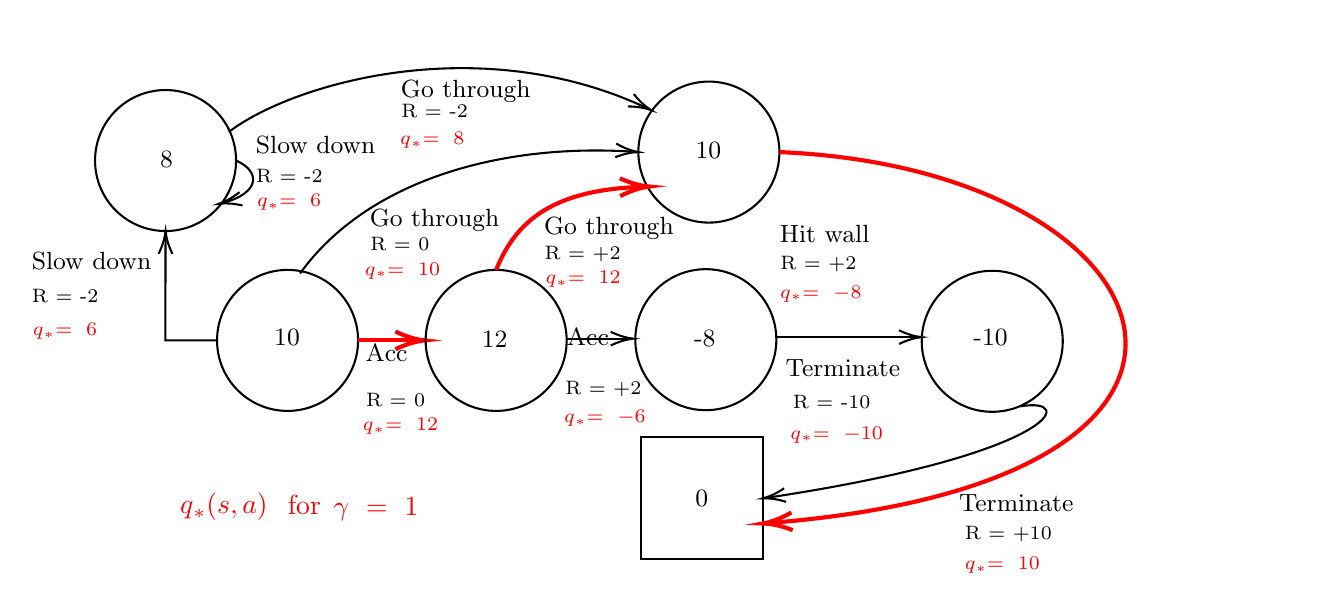
\begin{tikzpicture}[x=0.75pt,y=0.75pt,yscale=-1,xscale=1]
%uncomment if require: \path (0,300); %set diagram left start at 0, and has height of 300

%Shape: Rectangle [id:dp5992850543859389] 
\draw   (348.23,203.58) -- (406.71,203.58) -- (406.71,262.07) -- (348.23,262.07) -- cycle ;
%Shape: Ellipse [id:dp8590281199306287] 
\draw   (143.78,156.92) .. controls (143.78,138.16) and (158.99,122.95) .. (177.75,122.95) .. controls (196.51,122.95) and (211.72,138.16) .. (211.72,156.92) .. controls (211.72,175.69) and (196.51,190.89) .. (177.75,190.89) .. controls (158.99,190.89) and (143.78,175.69) .. (143.78,156.92) -- cycle ;
%Shape: Ellipse [id:dp0041116790647308665] 
\draw   (85,70.26) .. controls (85,51.49) and (100.21,36.29) .. (118.97,36.29) .. controls (137.73,36.29) and (152.94,51.49) .. (152.94,70.26) .. controls (152.94,89.02) and (137.73,104.23) .. (118.97,104.23) .. controls (100.21,104.23) and (85,89.02) .. (85,70.26) -- cycle ;
%Shape: Ellipse [id:dp2627001524161767] 
\draw   (346.77,66.19) .. controls (346.77,47.43) and (361.98,32.22) .. (380.74,32.22) .. controls (399.5,32.22) and (414.71,47.43) .. (414.71,66.19) .. controls (414.71,84.95) and (399.5,100.16) .. (380.74,100.16) .. controls (361.98,100.16) and (346.77,84.95) .. (346.77,66.19) -- cycle ;
%Shape: Ellipse [id:dp6773919980706278] 
\draw   (345.3,156.57) .. controls (345.3,137.81) and (360.5,122.6) .. (379.27,122.6) .. controls (398.03,122.6) and (413.24,137.81) .. (413.24,156.57) .. controls (413.24,175.33) and (398.03,190.54) .. (379.27,190.54) .. controls (360.5,190.54) and (345.3,175.33) .. (345.3,156.57) -- cycle ;
%Shape: Ellipse [id:dp308474257969483] 
\draw   (483.3,157.35) .. controls (483.3,138.59) and (498.51,123.38) .. (517.27,123.38) .. controls (536.03,123.38) and (551.24,138.59) .. (551.24,157.35) .. controls (551.24,176.11) and (536.03,191.32) .. (517.27,191.32) .. controls (498.51,191.32) and (483.3,176.11) .. (483.3,157.35) -- cycle ;
%Curve Lines [id:da5222555874558987] 
\draw [color={rgb, 255:red, 255; green, 0; blue, 0 }  ,draw opacity=1 ][line width=1.5]    (414.71,66.19) .. controls (607.43,74.18) and (667.91,225.78) .. (406.65,245.13) ;
\draw [shift={(406.65,245.13)}, rotate = 355.76] [color={rgb, 255:red, 255; green, 0; blue, 0 }  ,draw opacity=1 ][line width=1.5]    (14.21,-4.28) .. controls (9.04,-1.82) and (4.3,-0.39) .. (0,0) .. controls (4.3,0.39) and (9.04,1.82) .. (14.21,4.28)   ;
%Curve Lines [id:da8279234286020356] 
\draw    (530.83,188.69) .. controls (559.05,183.85) and (548.57,212.07) .. (406.65,233.04) ;
\draw [shift={(406.65,233.04)}, rotate = 351.6] [color={rgb, 255:red, 0; green, 0; blue, 0 }  ][line width=0.75]    (10.93,-3.29) .. controls (6.95,-1.4) and (3.31,-0.3) .. (0,0) .. controls (3.31,0.3) and (6.95,1.4) .. (10.93,3.29)   ;
%Straight Lines [id:da8999877796267308] 
\draw    (413.24,155.35) -- (481.3,155.35) ;
\draw [shift={(483.3,155.35)}, rotate = 180] [color={rgb, 255:red, 0; green, 0; blue, 0 }  ][line width=0.75]    (10.93,-3.29) .. controls (6.95,-1.4) and (3.31,-0.3) .. (0,0) .. controls (3.31,0.3) and (6.95,1.4) .. (10.93,3.29)   ;
%Straight Lines [id:da2902631162904139] 
\draw [color={rgb, 255:red, 255; green, 0; blue, 0 }  ,draw opacity=1 ][line width=1.5]    (211.72,156.92) -- (240.91,156.92) ;
\draw [shift={(243.91,156.92)}, rotate = 180] [color={rgb, 255:red, 255; green, 0; blue, 0 }  ,draw opacity=1 ][line width=1.5]    (14.21,-4.28) .. controls (9.04,-1.82) and (4.3,-0.39) .. (0,0) .. controls (4.3,0.39) and (9.04,1.82) .. (14.21,4.28)   ;
%Curve Lines [id:da4934773233251677] 
\draw    (152.94,70.26) .. controls (164.64,75.34) and (164.99,85.85) .. (146.45,90.69) ;
\draw [shift={(144.67,91.12)}, rotate = 347.2] [color={rgb, 255:red, 0; green, 0; blue, 0 }  ][line width=0.75]    (10.93,-3.29) .. controls (6.95,-1.4) and (3.31,-0.3) .. (0,0) .. controls (3.31,0.3) and (6.95,1.4) .. (10.93,3.29)   ;
%Curve Lines [id:da38644317862011146] 
\draw    (149.51,56.44) .. controls (180.19,33.09) and (270.49,6.75) .. (351.78,45.41) ;
\draw [shift={(353,46)}, rotate = 205.84] [color={rgb, 255:red, 0; green, 0; blue, 0 }  ][line width=0.75]    (10.93,-3.29) .. controls (6.95,-1.4) and (3.31,-0.3) .. (0,0) .. controls (3.31,0.3) and (6.95,1.4) .. (10.93,3.29)   ;
%Straight Lines [id:da99261008325772] 
\draw    (143.41,156.92) -- (118.87,156.92) -- (118.97,106.23) ;
\draw [shift={(118.97,104.23)}, rotate = 90.11] [color={rgb, 255:red, 0; green, 0; blue, 0 }  ][line width=0.75]    (10.93,-3.29) .. controls (6.95,-1.4) and (3.31,-0.3) .. (0,0) .. controls (3.31,0.3) and (6.95,1.4) .. (10.93,3.29)   ;
%Shape: Ellipse [id:dp14802512203998464] 
\draw   (244.28,156.92) .. controls (244.28,138.16) and (259.49,122.95) .. (278.25,122.95) .. controls (297.01,122.95) and (312.22,138.16) .. (312.22,156.92) .. controls (312.22,175.69) and (297.01,190.89) .. (278.25,190.89) .. controls (259.49,190.89) and (244.28,175.69) .. (244.28,156.92) -- cycle ;
%Straight Lines [id:da712075522965631] 
\draw    (312.22,156.07) -- (342.41,156.07) ;
\draw [shift={(344.41,156.07)}, rotate = 180] [color={rgb, 255:red, 0; green, 0; blue, 0 }  ][line width=0.75]    (10.93,-3.29) .. controls (6.95,-1.4) and (3.31,-0.3) .. (0,0) .. controls (3.31,0.3) and (6.95,1.4) .. (10.93,3.29)   ;
%Curve Lines [id:da4229873418348806] 
\draw [color={rgb, 255:red, 255; green, 0; blue, 0 }  ,draw opacity=1 ][line width=1.5]    (278.25,122.95) .. controls (289.16,95.52) and (310.66,84.22) .. (349.15,82.88) ;
\draw [shift={(352.14,82.8)}, rotate = 178.78] [color={rgb, 255:red, 255; green, 0; blue, 0 }  ,draw opacity=1 ][line width=1.5]    (14.21,-4.28) .. controls (9.04,-1.82) and (4.3,-0.39) .. (0,0) .. controls (4.3,0.39) and (9.04,1.82) .. (14.21,4.28)   ;
%Curve Lines [id:da33805841791197455] 
\draw    (183.76,124.67) .. controls (216.1,79.81) and (280.4,61.69) .. (344.82,66.05) ;
\draw [shift={(346.77,66.19)}, rotate = 184.28] [color={rgb, 255:red, 0; green, 0; blue, 0 }  ][line width=0.75]    (10.93,-3.29) .. controls (6.95,-1.4) and (3.31,-0.3) .. (0,0) .. controls (3.31,0.3) and (6.95,1.4) .. (10.93,3.29)   ;

% Text Node
\draw (161.04,56.81) node [anchor=north west][inner sep=0.75pt]  [font=\footnotesize] [align=left] {{\small Slow down}};
% Text Node
\draw (413.44,99.78) node [anchor=north west][inner sep=0.75pt]  [font=\footnotesize] [align=left] {{\small Hit wall}};
% Text Node
\draw (161.12,72.87) node [anchor=north west][inner sep=0.75pt]   [align=left] {{\scriptsize \textcolor[rgb]{0,0,0}{R = -2}}};
% Text Node
\draw (372.14,150.85) node [anchor=north west][inner sep=0.75pt]   [align=left] {{\small \textcolor[rgb]{0,0,0}{-8}}};
% Text Node
\draw (372.72,227.86) node [anchor=north west][inner sep=0.75pt]   [align=left] {{\small \textcolor[rgb]{0,0,0}{0}}};
% Text Node
\draw (416.27,164.81) node [anchor=north west][inner sep=0.75pt]  [font=\footnotesize] [align=left] {{\small Terminate}};
% Text Node
\draw (372.82,60.15) node [anchor=north west][inner sep=0.75pt]   [align=left] {{\small \textcolor[rgb]{0,0,0}{10}}};
% Text Node
\draw (506.73,150.38) node [anchor=north west][inner sep=0.75pt]   [align=left] {\textcolor[rgb]{0,0,0}{{\small -10}}};
% Text Node
\draw (176.36,230.2) node [anchor=north west][inner sep=0.75pt]   [align=left] {\textcolor[rgb]{1,0,0}{for}};
% Text Node
\draw (198.32,231.17) node [anchor=north west][inner sep=0.75pt]    {$\textcolor[rgb]{1,0,0}{\gamma\ =\ 1}$};
% Text Node
\draw (499.76,229.59) node [anchor=north west][inner sep=0.75pt]  [font=\footnotesize] [align=left] {{\small Terminate}};
% Text Node
\draw (502.54,244.78) node [anchor=north west][inner sep=0.75pt]   [align=left] {{\scriptsize \textcolor[rgb]{0,0,0}{R = +10}}};
% Text Node
\draw (419.73,181.94) node [anchor=north west][inner sep=0.75pt]   [align=left] {{\scriptsize \textcolor[rgb]{0,0,0}{R = -10}}};
% Text Node
\draw (413.73,114.94) node [anchor=north west][inner sep=0.75pt]   [align=left] {{\scriptsize \textcolor[rgb]{0,0,0}{R = +2}}};
% Text Node
\draw (230.87,30) node [anchor=north west][inner sep=0.75pt]  [font=\footnotesize] [align=left] {{\small Go through}};
% Text Node
\draw (231.12,41.87) node [anchor=north west][inner sep=0.75pt]   [align=left] {{\scriptsize \textcolor[rgb]{0,0,0}{R = -2}}};
% Text Node
\draw (215.87,92.07) node [anchor=north west][inner sep=0.75pt]  [font=\footnotesize] [align=left] {{\small Go through}};
% Text Node
\draw (216.12,105.93) node [anchor=north west][inner sep=0.75pt]   [align=left] {{\scriptsize \textcolor[rgb]{0,0,0}{R = 0}}};
% Text Node
\draw (299.87,96.07) node [anchor=north west][inner sep=0.75pt]  [font=\footnotesize] [align=left] {{\small Go through}};
% Text Node
\draw (300.12,109.93) node [anchor=north west][inner sep=0.75pt]   [align=left] {{\scriptsize \textcolor[rgb]{0,0,0}{R = +2}}};
% Text Node
\draw (310.87,145.07) node [anchor=north west][inner sep=0.75pt]  [font=\footnotesize] [align=left] {\begin{minipage}[lt]{14.97pt}\setlength\topsep{0pt}
\begin{center}
{\small Acc}
\end{center}

\end{minipage}};
% Text Node
\draw (213.87,153.07) node [anchor=north west][inner sep=0.75pt]  [font=\footnotesize] [align=left] {\begin{minipage}[lt]{14.97pt}\setlength\topsep{0pt}
\begin{center}
{\small Acc}
\end{center}

\end{minipage}};
% Text Node
\draw (269.82,151.15) node [anchor=north west][inner sep=0.75pt]   [align=left] {{\small \textcolor[rgb]{0,0,0}{12}}};
% Text Node
\draw (310.12,174.93) node [anchor=north west][inner sep=0.75pt]   [align=left] {{\scriptsize \textcolor[rgb]{0,0,0}{R = +2}}};
% Text Node
\draw (214.12,180.93) node [anchor=north west][inner sep=0.75pt]   [align=left] {{\scriptsize \textcolor[rgb]{0,0,0}{R = 0}}};
% Text Node
\draw (53.12,130.93) node [anchor=north west][inner sep=0.75pt]   [align=left] {{\scriptsize \textcolor[rgb]{0,0,0}{R = -2}}};
% Text Node
\draw (53.04,112.81) node [anchor=north west][inner sep=0.75pt]  [font=\footnotesize] [align=left] {{\small Slow down}};
% Text Node
\draw (169.82,150.15) node [anchor=north west][inner sep=0.75pt]   [align=left] {{\small \textcolor[rgb]{0,0,0}{10}}};
% Text Node
\draw (114.82,64.15) node [anchor=north west][inner sep=0.75pt]   [align=left] {{\small \textcolor[rgb]{0,0,0}{8}}};
% Text Node
\draw (124.54,229) node [anchor=north west][inner sep=0.75pt]    {$\textcolor[rgb]{1,0,0}{q}\textcolor[rgb]{1,0,0}{_{*}}\textcolor[rgb]{1,0,0}{(}\textcolor[rgb]{1,0,0}{s,a}\textcolor[rgb]{1,0,0}{)}$};
% Text Node
\draw (413.54,129) node [anchor=north west][inner sep=0.75pt]  [font=\scriptsize]  {${\textstyle \textcolor[rgb]{1,0,0}{q}\textcolor[rgb]{1,0,0}{_{*}}\textcolor[rgb]{1,0,0}{=\ -8}}$};
% Text Node
\draw (418.54,197) node [anchor=north west][inner sep=0.75pt]  [font=\scriptsize]  {${\textstyle \textcolor[rgb]{1,0,0}{q}\textcolor[rgb]{1,0,0}{_{*}}\textcolor[rgb]{1,0,0}{=\ -10}}$};
% Text Node
\draw (502.54,260) node [anchor=north west][inner sep=0.75pt]  [font=\scriptsize]  {${\textstyle \textcolor[rgb]{1,0,0}{q}\textcolor[rgb]{1,0,0}{_{*}}\textcolor[rgb]{1,0,0}{=\ 10}}$};
% Text Node
\draw (309.54,189) node [anchor=north west][inner sep=0.75pt]  [font=\scriptsize]  {${\textstyle \textcolor[rgb]{1,0,0}{q}\textcolor[rgb]{1,0,0}{_{*}}\textcolor[rgb]{1,0,0}{=\ -6}}$};
% Text Node
\draw (212.54,193) node [anchor=north west][inner sep=0.75pt]  [font=\scriptsize]  {${\textstyle \textcolor[rgb]{1,0,0}{q}\textcolor[rgb]{1,0,0}{_{*}}\textcolor[rgb]{1,0,0}{=\ 12}}$};
% Text Node
\draw (213.54,118) node [anchor=north west][inner sep=0.75pt]  [font=\scriptsize]  {${\textstyle \textcolor[rgb]{1,0,0}{q}\textcolor[rgb]{1,0,0}{_{*}}\textcolor[rgb]{1,0,0}{=\ 10}}$};
% Text Node
\draw (300.54,122) node [anchor=north west][inner sep=0.75pt]  [font=\scriptsize]  {${\textstyle \textcolor[rgb]{1,0,0}{q}\textcolor[rgb]{1,0,0}{_{*}}\textcolor[rgb]{1,0,0}{=\ 12}}$};
% Text Node
\draw (230.54,55) node [anchor=north west][inner sep=0.75pt]  [font=\scriptsize]  {${\textstyle \textcolor[rgb]{1,0,0}{q}\textcolor[rgb]{1,0,0}{_{*}}\textcolor[rgb]{1,0,0}{=\ 8}}$};
% Text Node
\draw (161.54,85) node [anchor=north west][inner sep=0.75pt]  [font=\scriptsize]  {${\textstyle \textcolor[rgb]{1,0,0}{q}\textcolor[rgb]{1,0,0}{_{*}}\textcolor[rgb]{1,0,0}{=\ 6}}$};
% Text Node
\draw (53.54,147) node [anchor=north west][inner sep=0.75pt]  [font=\scriptsize]  {${\textstyle \textcolor[rgb]{1,0,0}{q}\textcolor[rgb]{1,0,0}{_{*}}\textcolor[rgb]{1,0,0}{=\ 6}}$};
\end{tikzpicture}\caption{Optimal Policy of an MDP}
\label{optimalpolicymdp}
\end{figure}
 
As expected, the optimal policy for the car is to accelerate only once to go through the corner. Even though the example was trivial, the process is the same for all RL algorithms based on Q-Learning (Subsection \ref{qlearningsection}): The agent moves along the edges with the highest $q_*$, it maximises over $q_*(s,a)$.
\newline
Finally, the Bellman equations for $v_*$ and $q_*$ can be expressed as such (Equation \ref{bellmanoptimality}):
\begin{equation}
\label{bellmanoptimality}
	\begin{split}
		v_*(s) & = \underset{a}{max} \: q_*(s,a) \\
		& = \underset{a}{max} \: R_{s}^{a} + \gamma \sum\limits_{s \in S}P_{ss^{'}}^{a} v_*(s^{'}) \\
		q_*(s,a) & = R_{s}^{a} + \gamma \sum\limits_{s^{'} \in S} P_{ss^{'}}^{a} v_*(s^{'}) \\
		& = R_{s}^{a}+\gamma \sum\limits_{s^{'} \in S}P_{ss^{'}}^{a}\underset{a^{'}}{max} \: q_*(s^{'},a^{'})
	\end{split}
\end{equation}

MDPs can be extended to Partially Observable MDPs (POMDPs) that are a generalisation of MDPs, where the agent's observation is a subset of its state \cite{silver2015}. This represents a situation where the agent indirectly observes the environment: it could be a robot with a limited field of view or a trader with only limited access to financial market data. POMDPs can thus be represented as a tuple $\left< S,A,O,P,R,\gamma,Z \right>$ with $O$ a set of observations and $Z$ an observation function such as $Z_{s^{'}o}^{a} = \mathbb{P}[O_{t+1}=o \mid S_{t+1} = s^{'},A_t = a]$. The agent has its belief state $b(h)$, which is a probability distribution over all states conditioned on the agent's history $h$ (Equation \ref{belief}):
\begin{equation}
\label{belief}
b(h) = (\mathbb{P}[S_t = s^{1} \mid H_t = h ],...,\mathbb{P}[S_t = s^{n} \mid H_t = h])
\end{equation}
POMDPs can then be reduced as a history tree storing the succession of alternating actions and observations and a belief tree storing the probability of being in a state conditioned on this succession of actions and observations. \newline
In the case of autonomous racing with a model-based controller, the problem can be formalised as a POMDP \cite{modelbased}. The deterministic reward function $R$ is chosen to incentivise safe, smooth and fast control of the car, and the observation function $Z$ would, in our case, output the equivalent of a LiDAR scan with a limited field of view.


\subsection{Exploration vs. exploitation problem}
\label{explovsexplo}

One of the most fundamental questions of Reinforcement Learning is how an agent can compromise between exploration and exploitation. Exploitation consists of making the best decision given the current information (according to the agent's current value function). In contrast, exploration consists of doing something else to gather more information, which could lead to better rewards in the long run. \newline
The best long-term strategy would be a compromise between exploiting and exploring to avoid getting stuck in local minima; this is the same dilemma someone could face when deciding between going to their favourite restaurant or trying out a new one. There are three main approaches for compromising between exploration and exploitation (\cite{silver2015}): 
\begin{itemize}
	\item Random exploration (e.g. the softmax or the $\epsilon$-greedy algorithms, which introduces randomness into the action choice; this is the less sophisticated method.
	\item Optimism in the face of uncertainty: whenever the agent is uncertain about the value of an action, it should try it. The challenge is that the agent needs some way of measuring certainty; this is, however, a more ``rigorous" approach than random exploration.
	\item The most systematic approach but also the most computationally difficult is to consider the agent's information itself as part of its state (the agent might be in a state where it has never tried a specific action).
\end{itemize}


There are two spaces in which an agent can explore: the state-action space (taking different actions) and the parameter space (trying out different policy parameters for a parametrised policy $\pi(A|S,u)$; the advantage of exploring the parameter space is that the exploration is more consistent than state-action exploration; however the downside is that the learning process may take more time to converge because the agent doesn't know if it has already made an action before and may thus do the same action expecting different results. \newline
The exploration vs exploitation problem can be modelled as a multi-armed bandit process. A multi-armed bandit is a tuple $<A,R>$, with $A$ the known set of actions (``arms") and $R$ the unknown set of rewards. For each action there is an unknown reward defined by $R^{a}(r) = \mathbb{P}\left[R=r|A=a\right]$, and at each step $t$ the agent chooses an action $A_t \in A$. The environment then generates a reward $R_t \sim R^{A_t}$, and the goal of the agent is to maximise the cumulative reward $\sum_{\tau=1}^{t}R_{\tau}$. The action-value function gives the mean reward for an action $a$, defined by: $q(a)=\mathbb{E} \left[R|A=A\right]$; the optimal value is then defined as $v_*=q(a^{*}=\underset{a \in A}{max} \: q(a)$. The regret can then be defined as the loss of opportunity for one step: $I_t = \mathbb{E} \left[ v_* - q(A_t)\right]$; the total regret is then the total loss of opportunity over $t$ steps: $L_t = \mathbb{E} \Biggl[ \: \sum\limits_{\tau=1}^{t} v_* - q(A_{\tau})\Biggr]$. It should also be noted that maximising the cumulative reward is equivalent to minimising the total regret. The smaller the total regret, the better the policy is. \newline
We can now define the count $N_t(a)$ as the number of times an action $a$ has been selected, and the gap $\Delta_a$ as the difference in value between some action $a$ and the optimal action $a^{*}$: $\Delta_a = v_* - q(a)$. Regret can finally be defined as a function of gaps and counts (Equation \ref{regretfunction}): 
\begin{equation}
\label{regretfunction}
	\begin{split}
		L_t & = \mathbb{E} \Biggl[ \: \sum\limits_{\tau=1}^{t} v_* - q(A_{\tau})\Biggr] \\
		& = \sum\limits_{a \in A} \mathbb{E}\left[N_t(a)\right](v_*-q(a)) \\
		& = \sum\limits_{a \in A}\mathbb{E}\left[N_t(a)\right]\Delta_a
	\end{split}
\end{equation}

This definition can be understood as follows: we want to pick the actions (``arms") which are best as often as possible and the actions that are worst as infrequently as possible; the problem here is that the gaps are not known to the agent. \newline
The $\epsilon$-greedy algorithm that will be used in Algorithm \ref{dql} is a naive way of solving the exploration-exploitation problem: every time step there is a probability $\epsilon$ to select a random action and a probability $1-\epsilon$ to select $A = \underset{a \in A}{argmax} \: Q(a)$. Because $\epsilon$ is constant, it continues to explore the same way forever.


\section{Reinforcement Learning applied to autonomous racing}
\label{rlaracing}
\subsection{Q-Learning}
\label{qlearningsection}
\begin{algorithm}
\caption{Q-Learning: Learn function $Q: X \times A \rightarrow \mathbb{R}$, \cite{watkins1989}}
\label{qlearning}
\begin{algorithmic}[1]
\renewcommand{\algorithmicensure}{\textbf{Initialisation:}}
\Require
\Statex States $X = \left\{1,...,n_{x}\right\}$
\Statex Actions $A = \left\{1,...,n_{a}\right\} \: \: \: \: A : X \Rightarrow A$
\Statex Reward function $R: X \times A \rightarrow \mathbb{R}$
\Statex Transition function $T: X \times A \rightarrow X $
\Statex Learning rate $\alpha \in \left[0,1\right]$
\Statex Discount factor $\gamma \in \left[0,1\right]$
\Ensure $Q:X \times A \rightarrow \mathbb{R}$ with arbitrary values
\While{Q is not converged} \\
\hskip1.5em Initialise $s$
\While{$s$ is not terminal} \\
\hskip3.0em Choose $a$ from $s$ following a policy derived from $Q$ (e.g.the $\epsilon$-greedy policy) \label{epsilon}\\
\hskip3.0em $r \leftarrow R(s,a)$ \\
\hskip3.0em $s^{'} \leftarrow T(s,a)$ \\
\hskip3.0em	$Q(s,a) \leftarrow Q(s,a) + \alpha \left[ r + \gamma \: \max_{a^{'}} \: Q(s^{'},a^{'}) - Q(s,a) \right]$ \label{formula}\\
\hskip3.0em $s \leftarrow s^{'}$
\EndWhile
\EndWhile \\
\Return $Q$
\end{algorithmic}
\end{algorithm}


The Q-Learning algorithm introduced in \cite{watkins1989} is the most used model-free off-policy RL algorithm. With enough time and for any MDP, Q-Learning can determine the optimal action-selection policy, which was first rigorously proved in \cite{qlearningconvergence}. The algorithm is a function calculating the ``quality" of a state-action combination: $Q: S \times A \rightarrow \mathbb{R}$. This scalar value is the Q-value associated with the state-action combination. The training process can be imagined as updating the Q-values stored in a 2D table of state-actions combinations. The core of the Q-Learning algorithm is the Bellman equation, which updates the Q values. The new value of $Q$ is the sum of three different quantities: 

\begin{itemize}
	\item $(1-\alpha)Q(s_t,a_t)$, which is the current Q-value weighted with the learning rate $\alpha$
	\item $\alpha \: r_t$, which corresponds to the reward obtained if action $a_t$ is taken when the agent is in state $s_t$, multiplied by the learning rate
	\item $\alpha \: \gamma \: \underset{a}{max} \: Q(s_{t+1},a)$, which is the maximum reward possible from state $s_{t+1}$ multiplied by the learning rate and the discount factor
\end{itemize}

It is important to note that Q-Learning is off-policy because when updating the Q-value on line \ref{formula}, it uses the Q-value of the following state $s^{'}$ and the greedy action $a^{'}$. It doesn't matter that the policy followed to choose $a$ from $s$ on line \ref{epsilon} is not a greedy policy, Q-Learning will assume the agent is following a greedy policy nevertheless. This is similar to the Deep Deterministic Algorithm, which we will look at in section \ref{ddpgsection}.
The policy derived from $Q$ used to choose $a$ is sometimes an $\epsilon$-greedy policy, which was introduced in Subsection \ref{explovsexplo}. 
\newline
It is important to consider the learning rate $\alpha$, the discount factor $\gamma$ and the initial conditions $Q_0$.
\begin{itemize}
	\item With a learning rate of 0, the agent won't learn anything and will only exploit his prior knowledge. With $\alpha = 1$, it will only look at the most recent data. The learning rate can also be a function of time, decreasing when the training has progressed enough.
	\item $\gamma$ represents the compromise between short ($\gamma \rightarrow 0$) and long ($\gamma \rightarrow 1$) sightedness. The discount factor is generally chosen close to 1, starting with a lower factor and increasing it over time to accelerate the training.
	\item The initial conditions $Q_0$ are also important. If they are not carefully chosen, they may lead to a situation where states that have already been visited may have a value superior to states that haven't yet. The agent would thus explore less at the beginning of the training and get stuck.
\end{itemize}

\subsection{Deep Q-Learning}
\label{dqlearningsection}
Deep Q-Learning is an improvement over Q-Learning introduced by DeepMind in \cite{drl}. Their goal was to develop an algorithm that could solve a wide range of challenging tasks that cannot be handled with Q-Learning. The process combined RL with deep CNN to deal with never encountered states. The NN approximates the optimal action-value function representing the maximum sum of rewards $r_t$ with discount $\gamma$ achievable by a policy $\pi = P(a|s)$ after making an observation $s$ and an action $a$ (Equation \ref{optimalactionvaluefunctionapprox}):
\begin{equation}
\label{optimalactionvaluefunctionapprox}
	Q^{*}(s,a) = \underset{\pi}{max}\: \mathbb{E} \left[r_t + \gamma r_{t+1} + \gamma^{2} r_{t+2} + ... | s_t=s,a_t=a,\pi\right]
\end{equation}


 The algorithm has the following structure (Algorithm \ref{dql}):
	
\begin{algorithm}[H]
\caption{Deep Q-Learning with experience replay, \cite{drl}}
\label{dql}
\begin{algorithmic}[1]
\renewcommand{\algorithmicensure}{\textbf{Initialisation:}}
\Ensure
\Statex Initialise replay memory $R$ to capacity N
\Statex Initialise action-value function $Q(s,a,\theta)$ with random weights $\theta$
 \Statex Initialise target action-value function $Q_{target}$ with weights $\theta^{'} = \theta$
\For{episode = 1, episode $\leq M$} \\
\hskip1.0em Initialise state $s_t$
\For{$t = 1, t \leq T$} \\
\hskip3.0em Choose $a_t$ from $s_t$ following the $\epsilon$-greedy policy \\
\hskip3.0em Execute action $a_t$ and observe reward $r_t$ and new state $s_{t+1}$ \\
\hskip3.0em Store transition $(s_t,a_t,r_t,s_{t+1})$ in $R$ \label{buffer} \\
\hskip3.0em Set $s_{t+1} = s_t$ \\
\hskip3.0em Sample a random minibatch of N transitions $(s_i,a_i,r_i,s_{i+1})$ from $R$ \\
\hskip1.0em \begin{equation*}
\text{Set } y_i = \begin{cases}
	r_i & \text{for terminal state } s_{t+1} \\
	r_i + \gamma \: \underset{a^{'}}{max} \: Q_{target}\left(s_{t+1},a^{'},\theta \right) & \text{for non-terminal state } s_{t+1}
\end{cases}
\end{equation*} \label{targetupdate}\\ 
 \hskip3.0em Perform a gradient descent step on $\biggl( y_i - Q\biggl(s_t,a_i,\theta \biggr) \biggr)^{2}$ with respect to $\theta$ \\
\hskip3.0em Every $C$ steps reset $Q_{target} = Q$
\EndFor
\EndFor
\end{algorithmic}
\end{algorithm}

This algorithm differs from standard online Q-Learning in two ways. Firstly, it uses experience replay: the replay buffer stores the agent's experiences at each time-step (line \ref{buffer}) over many episodes. Inside the inner for-loop, the Q function is updated using a subset of experiences randomly sampled from the replay buffer. There are several advantages over online Q-Learning: an experience can be used several times for weight updates, which allows for greater data efficiency; it avoids overfitting by breaking the correlation between consecutively sampled experiences, and it helps avoid unwanted feedback loops that could stick the agent in a local minimum (\cite{temporaldiff}). Thus experience replay helps average the agent's behaviour by avoiding oscillations and divergences in $\theta$. \newline
The second difference with online Q-Learning is that the algorithm uses a different network $Q_{target}$ to generate the targets $y_i$ (line \ref{targetupdate}). Every $C$ step $Q_{target}$ is updated to $Q$, which creates a delay between the time $Q$ is updated and the time the update affects the targets $y_i$. Again, this is to avoid having diverging or oscillating parameters. As described in \cite{drl}, DeepMind reached super-human performance levels on several Atari games.

\subsection{Deep Deterministic Policy Gradient method}
\label{ddpgsection}
		%https://spinningup.openai.com/en/latest/algorithms/ddpg.html#background
		%(Silver 2014) http://proceedings.mlr.press/v32/silver14.pdf
		%Cont. Control with DRL: https://arxiv.org/pdf/1509.02971.pdf
		%https://www.youtube.com/watch?v=oydExwuuUCw&t=3s
		%https://markus-x-buchholz.medium.com/deep-reinforcement-learning-deep-deterministic-policy-gradient-ddpg-algoritm-5a823da91b43
		%https://www.katnoria.com/ddpg-reacher/
		
The Deep Deterministic Policy Gradient algorithm is a mode-free, off-policy algorithm, first introduced in \cite{ddpg2015}. It combines Deterministic Policy Gradients and Deep Q-Learning to learn a policy. As shown in Figure \ref{deterministic} Deterministic is opposed to stochastic: the policy takes a state as input and returns a single action; there are no probabilities involved. \newline
DDPG is thus both value-based (approximating the Q-function) and policy-based (using the Q-function to learn the policy): this can be seen in Figure \ref{taxonomy}. This approach is quite similar to Q-Learning: if the agents knows the optimal action-value function $Q^{*}(s,a)$, it can then find the optimal action $a^{*}(s)$ by solving: $a^{*}(s) = arg \: \underset{a}{max} \: Q^{*}(s,a)$.
The advantage of DDPG over Q-Learning is that it is adapted for continuous action spaces. This is related to the way $\underset{a}{max} \: Q^{*}(s,a)$ is computed: when there is only a finite number of actions, it is straightforward to compute by calculating the Q-values corresponding to all possible actions and selecting the best. In a continuous action space, we can consider the $Q^{*}(s,a)$ to be differentiable with respect to $a$, which lets us define $\mu(s)$, a rule to learn a policy. This way, $max_{a}Q(s,a)$ can be approximated as $max_{a}Q(s,a) \approx Q(s,\mu(s))$. \newline
We will now look at the equations involved in the part of DDPG that is learning the Q-function. The Bellman equation giving the optimal action-value function $Q^{*}$ is defined by Equation \ref{bellmanequation}:
\begin{equation}
\label{bellmanequation}
	Q^{*}(s,a) = \underset{s^{'} \sim P}{E}\left[r(s,a)+\gamma \: \underset{a^{'}}{max} \: Q^{*}(s^{'},a^{'})\right]
\end{equation}
		
Here, $ s^{'} \sim P $ means that the next state $ s^{'} $ is sampled by the environment from a probability distribution $P$. The Bellman equation is then used to learn the approximation of $ Q^{*} $.		
There are three main elements (Figure \ref{ddpg1}): 
\begin{enumerate}
	\item the actor network taking a state $s$ as input and returning an action $a$	
	\item the critic network taking as input a state $a$ and an action $a$ and returning the corresponding $Q_{value} = r + \gamma \: Q_{next}$ 
	\item the memory or replay buffer storing a subset of the past experiences of the agent: the state $s$, action $a$, reward associated $r$ and the next state $s$.It shouldn't contain too many previous experiences as that would make the training very slow but should be large enough to avoid overfitting.

\end{enumerate}

\begin{figure}[H]
\centering
\tikzset{every picture/.style={line width=0.75pt}} %set default line width to 0.75pt        

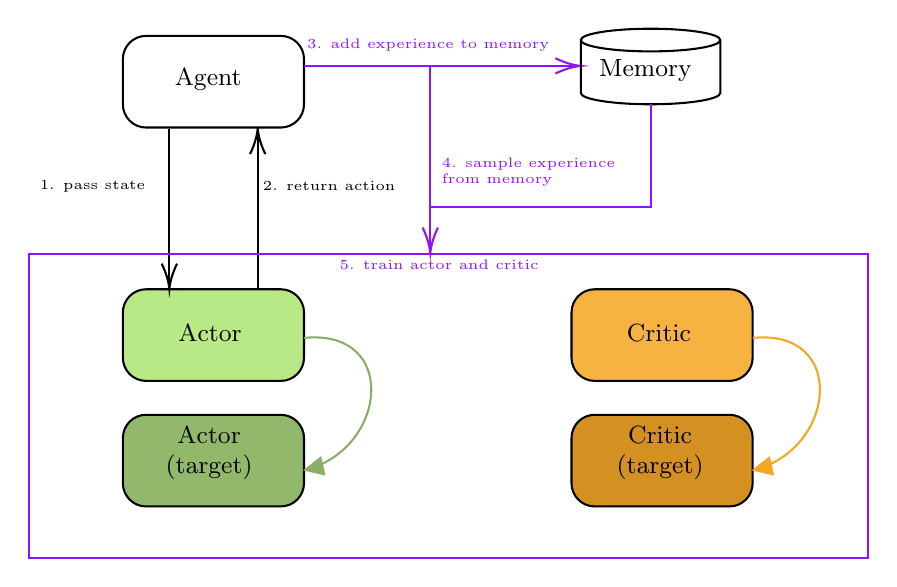
\begin{tikzpicture}[x=0.84pt,y=0.84pt,yscale=-1,xscale=1]
%uncomment if require: \path (0,300); %set diagram left start at 0, and has height of 300

%Shape: Rectangle [id:dp7952696348812505] 
\draw  [fill={rgb, 255:red, 184; green, 233; blue, 134 }  ,fill opacity=1 ] (179,170.08) .. controls (179,164.56) and (183.48,160.08) .. (189,160.08) -- (246.92,160.08) .. controls (252.44,160.08) and (256.92,164.56) .. (256.92,170.08) -- (256.92,189.51) .. controls (256.92,195.03) and (252.44,199.51) .. (246.92,199.51) -- (189,199.51) .. controls (183.48,199.51) and (179,195.03) .. (179,189.51) -- cycle ;
%Shape: Rectangle [id:dp15554819794274222] 
\draw  [fill={rgb, 255:red, 146; green, 184; blue, 107 }  ,fill opacity=1 ] (179,224.08) .. controls (179,218.56) and (183.48,214.08) .. (189,214.08) -- (246.92,214.08) .. controls (252.44,214.08) and (256.92,218.56) .. (256.92,224.08) -- (256.92,243.51) .. controls (256.92,249.03) and (252.44,253.51) .. (246.92,253.51) -- (189,253.51) .. controls (183.48,253.51) and (179,249.03) .. (179,243.51) -- cycle ;
%Curve Lines [id:da017965271262395] 
\draw [color={rgb, 255:red, 138; green, 174; blue, 101 }  ,draw opacity=1 ]   (257,181) .. controls (297.46,177.1) and (292.77,227.39) .. (259.14,237.32) ;
\draw [shift={(256.5,238)}, rotate = 347.47] [fill={rgb, 255:red, 138; green, 174; blue, 101 }  ,fill opacity=1 ][line width=0.08]  [draw opacity=0] (8.93,-4.29) -- (0,0) -- (8.93,4.29) -- cycle    ;
%Shape: Rectangle [id:dp22734882503903808] 
\draw  [fill={rgb, 255:red, 247; green, 179; blue, 66 }  ,fill opacity=1 ] (372,170.08) .. controls (372,164.56) and (376.48,160.08) .. (382,160.08) -- (439.92,160.08) .. controls (445.44,160.08) and (449.92,164.56) .. (449.92,170.08) -- (449.92,189.51) .. controls (449.92,195.03) and (445.44,199.51) .. (439.92,199.51) -- (382,199.51) .. controls (376.48,199.51) and (372,195.03) .. (372,189.51) -- cycle ;
%Shape: Rectangle [id:dp013800733069142535] 
\draw  [fill={rgb, 255:red, 212; green, 144; blue, 33 }  ,fill opacity=1 ] (372,224.08) .. controls (372,218.56) and (376.48,214.08) .. (382,214.08) -- (439.92,214.08) .. controls (445.44,214.08) and (449.92,218.56) .. (449.92,224.08) -- (449.92,243.51) .. controls (449.92,249.03) and (445.44,253.51) .. (439.92,253.51) -- (382,253.51) .. controls (376.48,253.51) and (372,249.03) .. (372,243.51) -- cycle ;
%Curve Lines [id:da18777168247137466] 
\draw [color={rgb, 255:red, 245; green, 166; blue, 35 }  ,draw opacity=1 ]   (450,181) .. controls (490.46,177.1) and (485.77,227.39) .. (452.14,237.32) ;
\draw [shift={(449.5,238)}, rotate = 347.47] [fill={rgb, 255:red, 245; green, 166; blue, 35 }  ,fill opacity=1 ][line width=0.08]  [draw opacity=0] (8.93,-4.29) -- (0,0) -- (8.93,4.29) -- cycle    ;
%Straight Lines [id:da5791379301264798] 
\draw    (199,91) -- (199,158) ;
\draw [shift={(199,160)}, rotate = 270] [color={rgb, 255:red, 0; green, 0; blue, 0 }  ][line width=0.75]    (10.93,-3.29) .. controls (6.95,-1.4) and (3.31,-0.3) .. (0,0) .. controls (3.31,0.3) and (6.95,1.4) .. (10.93,3.29)   ;
%Straight Lines [id:da7843284203482941] 
\draw    (237,93) -- (237,160) ;
\draw [shift={(237,91)}, rotate = 90] [color={rgb, 255:red, 0; green, 0; blue, 0 }  ][line width=0.75]    (10.93,-3.29) .. controls (6.95,-1.4) and (3.31,-0.3) .. (0,0) .. controls (3.31,0.3) and (6.95,1.4) .. (10.93,3.29)   ;
%Shape: Rectangle [id:dp5375441459348915] 
\draw  [fill={rgb, 255:red, 255; green, 255; blue, 255 }  ,fill opacity=1 ] (179,61.08) .. controls (179,55.56) and (183.48,51.08) .. (189,51.08) -- (246.92,51.08) .. controls (252.44,51.08) and (256.92,55.56) .. (256.92,61.08) -- (256.92,80.51) .. controls (256.92,86.03) and (252.44,90.51) .. (246.92,90.51) -- (189,90.51) .. controls (183.48,90.51) and (179,86.03) .. (179,80.51) -- cycle ;
%Straight Lines [id:da6784130396591115] 
\draw [color={rgb, 255:red, 144; green, 19; blue, 254 }  ,draw opacity=1 ]   (257,64) -- (374,64) ;
\draw [shift={(376,64)}, rotate = 180] [color={rgb, 255:red, 144; green, 19; blue, 254 }  ,draw opacity=1 ][line width=0.75]    (10.93,-3.29) .. controls (6.95,-1.4) and (3.31,-0.3) .. (0,0) .. controls (3.31,0.3) and (6.95,1.4) .. (10.93,3.29)   ;
%Shape: Can [id:dp28833945626088586] 
\draw   (436,52.88) -- (436,75.63) .. controls (436,78.32) and (422.57,80.5) .. (406,80.5) .. controls (389.43,80.5) and (376,78.32) .. (376,75.63) -- (376,52.88) .. controls (376,50.18) and (389.43,48) .. (406,48) .. controls (422.57,48) and (436,50.18) .. (436,52.88) .. controls (436,55.57) and (422.57,57.75) .. (406,57.75) .. controls (389.43,57.75) and (376,55.57) .. (376,52.88) ;
%Straight Lines [id:da8895063366590392] 
\draw [color={rgb, 255:red, 144; green, 19; blue, 254 }  ,draw opacity=1 ]   (311.25,64) -- (311.25,142.5) ;
\draw [shift={(311.25,144.5)}, rotate = 270] [color={rgb, 255:red, 144; green, 19; blue, 254 }  ,draw opacity=1 ][line width=0.75]    (10.93,-3.29) .. controls (6.95,-1.4) and (3.31,-0.3) .. (0,0) .. controls (3.31,0.3) and (6.95,1.4) .. (10.93,3.29)   ;
%Shape: Rectangle [id:dp8495843342833065] 
\draw  [color={rgb, 255:red, 144; green, 19; blue, 254 }  ,draw opacity=1 ] (138.5,145) -- (499.5,145) -- (499.5,275.5) -- (138.5,275.5) -- cycle ;
%Straight Lines [id:da7536728210571089] 
\draw [color={rgb, 255:red, 144; green, 19; blue, 254 }  ,draw opacity=1 ]   (406,80.5) -- (406,124.5) -- (311,124.5) ;

% Text Node
\draw (201.53,173.77) node [anchor=north west][inner sep=0.75pt]  [font=\small] [align=left] {Actor};
% Text Node
\draw (195.53,217.77) node [anchor=north west][inner sep=0.75pt]  [font=\small] [align=left] {\begin{minipage}[lt]{32.31pt}\setlength\topsep{0pt}
\begin{center}
Actor\\(target)
\end{center}

\end{minipage}};
% Text Node
\draw (394.53,173.77) node [anchor=north west][inner sep=0.75pt]  [font=\small] [align=left] {Critic};
% Text Node
\draw (389.53,217.77) node [anchor=north west][inner sep=0.75pt]  [font=\small] [align=left] {\begin{minipage}[lt]{32.31pt}\setlength\topsep{0pt}
\begin{center}
Critic\\(target)
\end{center}

\end{minipage}};
% Text Node
\draw (199.99,63.77) node [anchor=north west][inner sep=0.75pt]  [font=\small] [align=left] {Agent};
% Text Node
\draw (382.53,59.77) node [anchor=north west][inner sep=0.75pt]  [font=\small] [align=left] {Memory};
% Text Node
\draw (256.92,51.08) node [anchor=north west][inner sep=0.75pt]  [font=\tiny,color={rgb, 255:red, 144; green, 19; blue, 254 }  ,opacity=1 ] [align=left] {3. add experience to memory};
% Text Node
\draw (314.92,102.08) node [anchor=north west][inner sep=0.75pt]  [font=\tiny,color={rgb, 255:red, 144; green, 19; blue, 254 }  ,opacity=1 ] [align=left] {4. sample experience\\from memory};
% Text Node
\draw (270.92,146.08) node [anchor=north west][inner sep=0.75pt]  [font=\tiny,color={rgb, 255:red, 144; green, 19; blue, 254 }  ,opacity=1 ] [align=left] {5. train actor and critic};
% Text Node
\draw (141.92,112.08) node [anchor=north west][inner sep=0.75pt]  [font=\tiny,color={rgb, 255:red, 0; green, 0; blue, 0 }  ,opacity=1 ] [align=left] {1. pass state};
% Text Node
\draw (237.92,112.08) node [anchor=north west][inner sep=0.75pt]  [font=\tiny,color={rgb, 255:red, 0; green, 0; blue, 0 }  ,opacity=1 ] [align=left] {2. return action};
\end{tikzpicture}\caption{Deep Deterministic Policy Algorithm Process}
\label{ddpg1}
\end{figure}

It is important to note here that, like Q-Learning, DDPG is an off-policy algorithm which means that the learning proceeds not from actions taken using the current policy $ \pi(a|s)$ but from possibly outdated policies from the replay buffer. This is possible because, as demonstrated in \cite{watkins1989}, the Q-value of the following state $s^{'}$ contained in the Bellman equation is obtained following the greedy action $a^{'}$; it estimates the return for a state-action pair assuming a greedy policy is followed. This is why the Bellman equation is not concerned about the current policy and thus why DDPG is an off-policy algorithm. It is also important to note that because DDPG is off-policy, it should be more stable than on-policy methods, although it should converge slower.
\newline
The detailed training process is presented in Figure \ref{ddpggeneral}: \newline

\begin{figure}[H]
\centering
\tikzset{every picture/.style={line width=0.75pt}} %set default line width to 0.75pt        

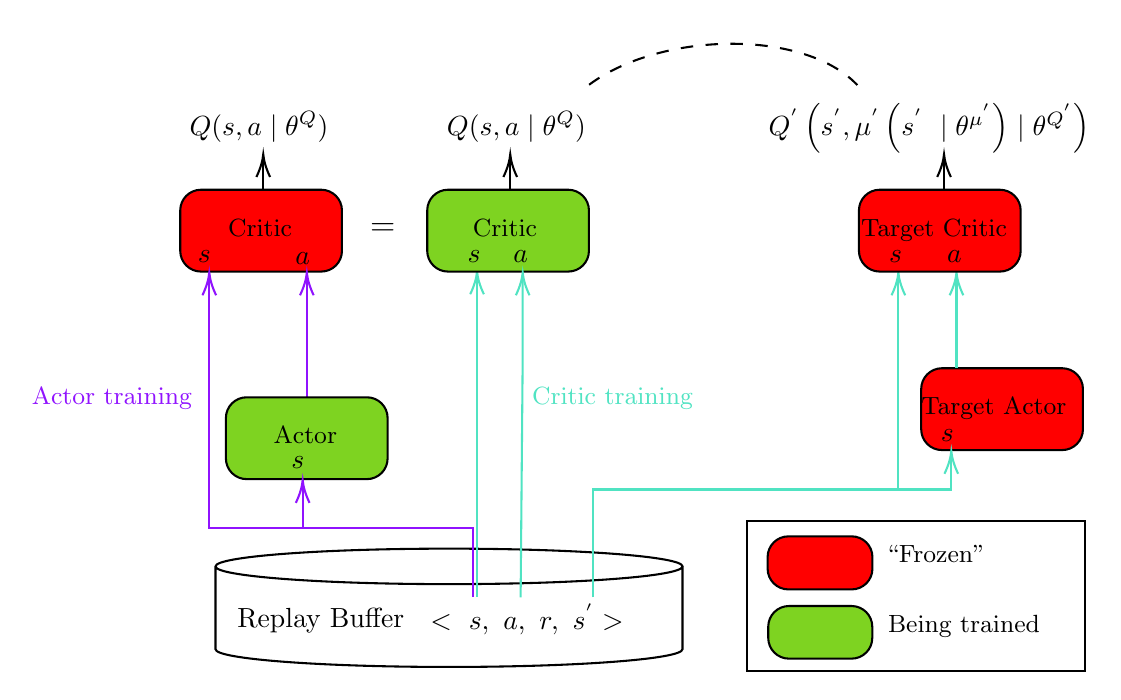
\begin{tikzpicture}[x=0.75pt,y=0.75pt,yscale=-1,xscale=1]
%uncomment if require: \path (0,300); %set diagram left start at 0, and has height of 300

%Shape: Rectangle [id:dp5480773364157583] 
\draw  [fill={rgb, 255:red, 255; green, 0; blue, 0 }  ,fill opacity=1 ] (78,76.08) .. controls (78,70.56) and (82.48,66.08) .. (88,66.08) -- (145.92,66.08) .. controls (151.44,66.08) and (155.92,70.56) .. (155.92,76.08) -- (155.92,95.51) .. controls (155.92,101.03) and (151.44,105.51) .. (145.92,105.51) -- (88,105.51) .. controls (82.48,105.51) and (78,101.03) .. (78,95.51) -- cycle ;
%Straight Lines [id:da47936409519792056] 
\draw    (118,51) -- (118,66) ;
\draw [shift={(118,49)}, rotate = 90] [color={rgb, 255:red, 0; green, 0; blue, 0 }  ][line width=0.75]    (10.93,-3.29) .. controls (6.95,-1.4) and (3.31,-0.3) .. (0,0) .. controls (3.31,0.3) and (6.95,1.4) .. (10.93,3.29)   ;
%Shape: Can [id:dp11846724225449012] 
\draw   (320,247.55) -- (320,287.45) .. controls (320,292.17) and (269.63,296) .. (207.5,296) .. controls (145.37,296) and (95,292.17) .. (95,287.45) -- (95,247.55) .. controls (95,242.83) and (145.37,239) .. (207.5,239) .. controls (269.63,239) and (320,242.83) .. (320,247.55) .. controls (320,252.27) and (269.63,256.1) .. (207.5,256.1) .. controls (145.37,256.1) and (95,252.27) .. (95,247.55) ;
%Straight Lines [id:da957594508249656] 
\draw [color={rgb, 255:red, 144; green, 19; blue, 254 }  ,draw opacity=1 ]   (92,108) -- (92,229) -- (219,229) -- (219,262.5) ;
\draw [shift={(92,106)}, rotate = 90] [color={rgb, 255:red, 144; green, 19; blue, 254 }  ,draw opacity=1 ][line width=0.75]    (10.93,-3.29) .. controls (6.95,-1.4) and (3.31,-0.3) .. (0,0) .. controls (3.31,0.3) and (6.95,1.4) .. (10.93,3.29)   ;
%Straight Lines [id:da6567166422281674] 
\draw [color={rgb, 255:red, 144; green, 19; blue, 254 }  ,draw opacity=1 ]   (139,108) -- (139,166) ;
\draw [shift={(139,106)}, rotate = 90] [color={rgb, 255:red, 144; green, 19; blue, 254 }  ,draw opacity=1 ][line width=0.75]    (10.93,-3.29) .. controls (6.95,-1.4) and (3.31,-0.3) .. (0,0) .. controls (3.31,0.3) and (6.95,1.4) .. (10.93,3.29)   ;
%Shape: Rectangle [id:dp2852540908279466] 
\draw  [fill={rgb, 255:red, 126; green, 211; blue, 33 }  ,fill opacity=1 ] (100,176.08) .. controls (100,170.56) and (104.48,166.08) .. (110,166.08) -- (167.92,166.08) .. controls (173.44,166.08) and (177.92,170.56) .. (177.92,176.08) -- (177.92,195.51) .. controls (177.92,201.03) and (173.44,205.51) .. (167.92,205.51) -- (110,205.51) .. controls (104.48,205.51) and (100,201.03) .. (100,195.51) -- cycle ;
%Straight Lines [id:da9658144353378741] 
\draw [color={rgb, 255:red, 144; green, 19; blue, 254 }  ,draw opacity=1 ]   (137,208) -- (137,229) ;
\draw [shift={(137,206)}, rotate = 90] [color={rgb, 255:red, 144; green, 19; blue, 254 }  ,draw opacity=1 ][line width=0.75]    (10.93,-3.29) .. controls (6.95,-1.4) and (3.31,-0.3) .. (0,0) .. controls (3.31,0.3) and (6.95,1.4) .. (10.93,3.29)   ;
%Shape: Rectangle [id:dp7138401871622682] 
\draw  [fill={rgb, 255:red, 255; green, 0; blue, 0 }  ,fill opacity=1 ] (361,243.08) .. controls (361,237.56) and (365.48,233.08) .. (371,233.08) -- (401.5,233.08) .. controls (407.02,233.08) and (411.5,237.56) .. (411.5,243.08) -- (411.5,248.64) .. controls (411.5,254.16) and (407.02,258.64) .. (401.5,258.64) -- (371,258.64) .. controls (365.48,258.64) and (361,254.16) .. (361,248.64) -- cycle ;
%Shape: Rectangle [id:dp017270935324260384] 
\draw  [fill={rgb, 255:red, 126; green, 211; blue, 33 }  ,fill opacity=1 ] (361.3,276.64) .. controls (361.3,271.11) and (365.78,266.64) .. (371.3,266.64) -- (401.43,266.64) .. controls (406.95,266.64) and (411.43,271.11) .. (411.43,276.64) -- (411.43,282) .. controls (411.43,287.52) and (406.95,292) .. (401.43,292) -- (371.3,292) .. controls (365.78,292) and (361.3,287.52) .. (361.3,282) -- cycle ;
%Straight Lines [id:da08142072925618704] 
\draw [color={rgb, 255:red, 80; green, 227; blue, 194 }  ,draw opacity=1 ]   (221,107.5) -- (221,223) -- (221,223) -- (221,262.5) ;
\draw [shift={(221,105.5)}, rotate = 90] [color={rgb, 255:red, 80; green, 227; blue, 194 }  ,draw opacity=1 ][line width=0.75]    (10.93,-3.29) .. controls (6.95,-1.4) and (3.31,-0.3) .. (0,0) .. controls (3.31,0.3) and (6.95,1.4) .. (10.93,3.29)   ;
%Shape: Rectangle [id:dp5606017772794614] 
\draw  [fill={rgb, 255:red, 126; green, 211; blue, 33 }  ,fill opacity=1 ] (197,76.08) .. controls (197,70.56) and (201.48,66.08) .. (207,66.08) -- (264.92,66.08) .. controls (270.44,66.08) and (274.92,70.56) .. (274.92,76.08) -- (274.92,95.51) .. controls (274.92,101.03) and (270.44,105.51) .. (264.92,105.51) -- (207,105.51) .. controls (201.48,105.51) and (197,101.03) .. (197,95.51) -- cycle ;
%Straight Lines [id:da8832023872930412] 
\draw [color={rgb, 255:red, 80; green, 227; blue, 194 }  ,draw opacity=1 ]   (243,108) -- (243,146.5) -- (243,146.5) -- (242,262.5) ;
\draw [shift={(243,106)}, rotate = 90] [color={rgb, 255:red, 80; green, 227; blue, 194 }  ,draw opacity=1 ][line width=0.75]    (10.93,-3.29) .. controls (6.95,-1.4) and (3.31,-0.3) .. (0,0) .. controls (3.31,0.3) and (6.95,1.4) .. (10.93,3.29)   ;
%Straight Lines [id:da23286438505502893] 
\draw    (237,51) -- (237,66) ;
\draw [shift={(237,49)}, rotate = 90] [color={rgb, 255:red, 0; green, 0; blue, 0 }  ][line width=0.75]    (10.93,-3.29) .. controls (6.95,-1.4) and (3.31,-0.3) .. (0,0) .. controls (3.31,0.3) and (6.95,1.4) .. (10.93,3.29)   ;
%Curve Lines [id:da5875523477074087] 
\draw  [dash pattern={on 4.5pt off 4.5pt}]  (275,15.5) .. controls (310,-10.5) and (380,-11.5) .. (405,16.5) ;
%Straight Lines [id:da7376949349118056] 
\draw    (446,51) -- (446,66) ;
\draw [shift={(446,49)}, rotate = 90] [color={rgb, 255:red, 0; green, 0; blue, 0 }  ][line width=0.75]    (10.93,-3.29) .. controls (6.95,-1.4) and (3.31,-0.3) .. (0,0) .. controls (3.31,0.3) and (6.95,1.4) .. (10.93,3.29)   ;
%Shape: Rectangle [id:dp28966980813208365] 
\draw  [fill={rgb, 255:red, 255; green, 0; blue, 0 }  ,fill opacity=1 ] (435,162.08) .. controls (435,156.56) and (439.48,152.08) .. (445,152.08) -- (502.92,152.08) .. controls (508.44,152.08) and (512.92,156.56) .. (512.92,162.08) -- (512.92,181.51) .. controls (512.92,187.03) and (508.44,191.51) .. (502.92,191.51) -- (445,191.51) .. controls (439.48,191.51) and (435,187.03) .. (435,181.51) -- cycle ;
%Straight Lines [id:da1508509898861019] 
\draw [color={rgb, 255:red, 80; green, 227; blue, 194 }  ,draw opacity=1 ]   (452,108) -- (452,152) ;
\draw [shift={(452,106)}, rotate = 90] [color={rgb, 255:red, 80; green, 227; blue, 194 }  ,draw opacity=1 ][line width=0.75]    (10.93,-3.29) .. controls (6.95,-1.4) and (3.31,-0.3) .. (0,0) .. controls (3.31,0.3) and (6.95,1.4) .. (10.93,3.29)   ;
%Straight Lines [id:da608810072044685] 
\draw [color={rgb, 255:red, 80; green, 227; blue, 194 }  ,draw opacity=1 ]   (277,262.5) -- (277,210.5) -- (424,210.5) -- (424,108) ;
\draw [shift={(424,106)}, rotate = 90] [color={rgb, 255:red, 80; green, 227; blue, 194 }  ,draw opacity=1 ][line width=0.75]    (10.93,-3.29) .. controls (6.95,-1.4) and (3.31,-0.3) .. (0,0) .. controls (3.31,0.3) and (6.95,1.4) .. (10.93,3.29)   ;
%Straight Lines [id:da40348636603297305] 
\draw [color={rgb, 255:red, 80; green, 227; blue, 194 }  ,draw opacity=1 ]   (424,210.5) -- (449.5,210.5) -- (449.5,194) ;
\draw [shift={(449.5,192)}, rotate = 90] [color={rgb, 255:red, 80; green, 227; blue, 194 }  ,draw opacity=1 ][line width=0.75]    (10.93,-3.29) .. controls (6.95,-1.4) and (3.31,-0.3) .. (0,0) .. controls (3.31,0.3) and (6.95,1.4) .. (10.93,3.29)   ;
%Shape: Rectangle [id:dp8383603070821517] 
\draw  [fill={rgb, 255:red, 255; green, 0; blue, 0 }  ,fill opacity=1 ] (405,76.08) .. controls (405,70.56) and (409.48,66.08) .. (415,66.08) -- (472.92,66.08) .. controls (478.44,66.08) and (482.92,70.56) .. (482.92,76.08) -- (482.92,95.51) .. controls (482.92,101.03) and (478.44,105.51) .. (472.92,105.51) -- (415,105.51) .. controls (409.48,105.51) and (405,101.03) .. (405,95.51) -- cycle ;
%Shape: Rectangle [id:dp6322969899464324] 
\draw   (351.25,225.86) -- (514,225.86) -- (514,298) -- (351.25,298) -- cycle ;

% Text Node
\draw (99.53,78.77) node [anchor=north west][inner sep=0.75pt]  [font=\small,color={rgb, 255:red, 0; green, 0; blue, 0 }  ,opacity=1 ] [align=left] {Critic};
% Text Node
\draw (104,266) node [anchor=north west][inner sep=0.75pt]   [align=left] {Replay Buffer};
% Text Node
\draw (197,264) node [anchor=north west][inner sep=0.75pt]    {$< \ s,\ a,\ r,\ s^{'}  >$};
% Text Node
\draw (85,94) node [anchor=north west][inner sep=0.75pt]    {$s$};
% Text Node
\draw (132,95) node [anchor=north west][inner sep=0.75pt]    {$a$};
% Text Node
\draw (121.53,178.77) node [anchor=north west][inner sep=0.75pt]  [font=\small] [align=left] {Actor};
% Text Node
\draw (130,193) node [anchor=north west][inner sep=0.75pt]    {$s$};
% Text Node
\draw (417.53,269.77) node [anchor=north west][inner sep=0.75pt]  [font=\small] [align=left] {Being trained};
% Text Node
\draw (416.53,235.77) node [anchor=north west][inner sep=0.75pt]  [font=\small] [align=left] {``Frozen"};
% Text Node
\draw (217.53,78.77) node [anchor=north west][inner sep=0.75pt]  [font=\small,color={rgb, 255:red, 0; green, 0; blue, 0 }  ,opacity=1 ] [align=left] {Critic};
% Text Node
\draw (215,94) node [anchor=north west][inner sep=0.75pt]    {$s$};
% Text Node
\draw (236.96,93.8) node [anchor=north west][inner sep=0.75pt]    {$a$};
% Text Node
\draw (418,94) node [anchor=north west][inner sep=0.75pt]    {$s$};
% Text Node
\draw (445.96,93.8) node [anchor=north west][inner sep=0.75pt]    {$a$};
% Text Node
\draw (360,23) node [anchor=north west][inner sep=0.75pt]    {$Q^{'}\left( s^{'}, \mu^{'}\left(s^{'} \mid \theta^{\mu^{'}} \right) \mid \theta^{Q^{'}}\right)$};
% Text Node
\draw (205,27) node [anchor=north west][inner sep=0.75pt]    {$Q( s,a \mid \theta^{Q})$};
% Text Node
\draw (433.53,164.77) node [anchor=north west][inner sep=0.75pt]  [font=\small,color={rgb, 255:red, 0; green, 0; blue, 0 }  ,opacity=1 ] [align=left] {Target Actor};
% Text Node
\draw (443,180) node [anchor=north west][inner sep=0.75pt]    {$s$};
% Text Node
\draw (404.53,78.77) node [anchor=north west][inner sep=0.75pt]  [font=\small,color={rgb, 255:red, 0; green, 0; blue, 0 }  ,opacity=1 ] [align=left] {Target Critic};
% Text Node
\draw (168,81) node [anchor=north west][inner sep=0.75pt]  [font=\large]  {$=$};
% Text Node
\draw (5,160) node [anchor=north west][inner sep=0.75pt]  [font=\small,color={rgb, 255:red, 144; green, 19; blue, 254 }  ,opacity=1 ] [align=left] {Actor training};
% Text Node
\draw (246,160) node [anchor=north west][inner sep=0.75pt]  [font=\small,color={rgb, 255:red, 80; green, 227; blue, 194 }  ,opacity=1 ] [align=left] {Critic training};
% Text Node
\draw (81,27) node [anchor=north west][inner sep=0.75pt]    {$Q(s,a \mid \theta^{Q})$};


\end{tikzpicture}
\caption{Detailed training process of the DDPG algorithm}
\label{ddpggeneral}
\end{figure}

We will now consider the detailed training process (Figure \ref{ddpggeneral}). We will look first at the training of the actor network. Assuming we have the critic network already trained, the observation from the replay buffer is fed into the actor and the critic, and the output action of the actor is fed into the critic network. The goal is then to maximise the Q-value output of the critic network. \newline
We have to use a copy of the critic and the actor networks to train the critic network. We feed into the actor and the critic the following observation, and the output of the actor network, which is the following action, is fed into the critic network. The critic outputs $Q_{next}$; this $Q_{next}$ is then compared to the Q value output of the target critic network fed by the observation and action of the replay buffer. The goal here is to minimise $ | Q - (r + \gamma \cdot Q_{next})|$, with the discount factor $ \gamma $ a hyper-parameter of the algorithm and the reward $r$ stored in the replay buffer (and corresponding to the action $a$). This is the part where the target critic and actor are necessary because without them; the problem would be that the critic and the actor would depend on the same parameters ($\theta^{Q}$ for the critic and $\theta^{\mu}$ for the actor) that we are trying to train, which would make the algorithm unstable. The target networks with parameters $\theta^{Q^{'}}$ for the critic and $\theta^{\mu^{'}}$ for the actor are lagging the actor and critic networks by one time-step and are updated as such (Equation \ref{thetaupdate}):
\begin{equation}
\label{thetaupdate}
	 \theta^{'} \leftarrow \rho \: \theta^{'} + (1- \rho)\theta
\end{equation}
with $\rho$ a hyper-parameter between 0 and 1. The whole training process is summarised in Algorithm \ref{ddpgalgo}. \newline
For the policy training part (the training of the actor network), we want to learn a deterministic policy $\mu_{\theta}$ which will maximise $Q(s,a\mid \theta^{\mu})$. For the Q-Learning part (the training of the critic network), we want to minimise the difference in Equation \ref{difference}:
\begin{equation}
\label{difference}
 \left(r + \gamma \: Q^{'}(s,\mu^{'}\left(s \mid \theta^{\mu^{'}}\right) \mid \theta^{Q^{'}}\right) - Q\left(s,a \mid \theta^{Q}\right)
\end{equation}
  Assuming we are approximating using a NN $ Q(s,a\mid \theta^{Q}) $ with $ \theta^{Q} $ the parameters and that we are storing in a replay buffer $R$ the following variables: $ \left< s,a,r,s^{'} \right>$, we can set-up a mean-squared Bellman error function (Equation \ref{bellmanerrorfunction}), with the goal of minimising it:
  \begin{equation}
  \label{bellmanerrorfunction}
  L(\theta,R) = \underset{(s,a,r,s^{'}) \sim R}{\mathbb{E}} \left[\left(r + \gamma Q^{'}\left(s^{'},\mu^{'}\left(s^{'}\mid \theta^{\mu^{'}}\right) \mid \theta^{Q^{'}} \right) - Q(s,a \mid \theta^{Q} \right)^{2}\right]  	
  \end{equation}

				
\begin{algorithm}
\caption{Deep Deterministic Policy Gradient, \cite{ddpg2015}}
\label{ddpgalgo}
\begin{algorithmic}[1]
\renewcommand{\algorithmicrequire}{\textbf{Input:}}
\renewcommand{\algorithmicensure}{\textbf{Initialisation:}}
\Require random initial weights $\theta^{Q}$ for critic network $Q(s,a|\theta^{Q})$ and $\theta^{\mu}$ for actor network $\mu(s|\theta^{\mu})$ \\
 Initialise target network $Q^{'}$ and $\mu^{'}$ with weights $\theta^{Q^{'}} \leftarrow \theta^{Q}$, $\theta^{\mu^{'}} \leftarrow \theta^{\mu}$ \\
 Initialise empty replay buffer $R$
 Initialise a random process $N$ for action exploration \\
 Receive initial observation state $s_1$
\For{$t = 1, t \leq T$} \\
\hskip1.0em Select action $a_t = \mu(s_t|\theta^{\mu}) + N_t$ according to current policy and exploration noise \\
\hskip1.0em Execute action $a_t$ and observe reward $r_t$ and new state $s_{t+1}$ \\
\hskip1.0em Store transition $(s_t,a_t,r_t,s_{t+1})$ in $R$ \\
\hskip1.0em Sample a random minibatch of N transitions $(s_i,a_i,r_i,s_{i+1})$ from $R$ \\
\hskip1.0em Set $y_i = r_i + \gamma Q^{'}\left(s_{i+1},\mu^{'}\left(s_{i+1}\mid\theta^{\mu^{'}}\right)\mid\theta^{Q^{'}}\right)$ \label{targetactionvalue}\\
\hskip1.0em Update critic by minimising the loss: $L = \frac{1}{N} \sum_i \left( y_i - Q(s_i,a_i \mid \theta^{Q})\right)^{2}$ \label{loss}\\
\hskip1.0em Update the actor policy using the sampled policy gradient: 
\begin{equation*}
	\nabla_{\theta^{\mu}}J \approx \frac{1}{N} \sum\limits_{i}\nabla_a Q\left(s,a \mid \theta^{Q}\right) \mid_{s=s_i,a=\mu(s_i)}\nabla_{\theta^{\mu}}\mu(s \mid \theta^{\mu}) \mid_{s_i}
\end{equation*} \label{spgradient}\\

\hskip1.0em Update the target networks: 
\begin{equation*}
	\theta^{Q^{'}} \leftarrow \tau\theta^{Q} + (1-\tau)\theta^{Q^{'}}
\end{equation*}
\begin{equation*}
	\theta^{\mu^{'}} \leftarrow \tau\theta^{\mu} + (1-\tau)\theta^{\mu^{'}}
\end{equation*} \label{updatetgttnet}
\EndFor
\end{algorithmic}
\end{algorithm}



Line \ref{loss}, the loss is given by the average of the squared differences between the target action-value $y_i$ and the expected action-value $Q\left(s_i,a_i \mid \theta^{Q}\right)$, with the expected action-value being given by the critic network $Q$. Line \ref{targetactionvalue}, the target action-value is calculated as the sum of the reward $r_i$ and the discounted action-value where the target critic network $Q^{'}$ takes the state $s_{i+1}$ and the action returned by the target actor $\mu^{'}$, mapping the state $s_{i+1}$ to the action $\mu^{'}\left(s_{i+1} \mid \theta^{\mu^{'}}\right)$. \newline
Then line \ref{spgradient} the actor is updated with the sampled policy gradient, which is the average of the action values given by the critic $Q$ with parameters $\theta^{Q}$ that takes the state $s$ and the action $a$ as input, where the action 
\newline
Finally, line \ref{updatetgttnet}, the algorithm uses the coefficient $\tau, \: \: \tau \ll 1$ to make the weights $\theta^{Q^{'}}$ and $\theta^{\mu^{'}}$ change slowly instead of directly copying $\theta^{Q}$ and $\theta^{\mu}$, which improves the stability of the process.


\section{Neural Networks}
\label{nns}
\subsection{Multi-Layer Perceptron}
\label{mlpsection}

The Multi-Layer Perceptron (MLP) is a type of NN composed of perceptrons. The advantage over a simple perceptron is that a perceptron is a linear classifier, whereas an MLP is non-linear and can classify classes that are not linearly separable. The perceptrons are organised in at least three layers: the input layer, one or more hidden layers and the output layer. In the example Figure \ref{mlp}, each connection between nodes is represented in a shade of grey depending on the value of the associated weight.

\begin{figure}[H]
\centering
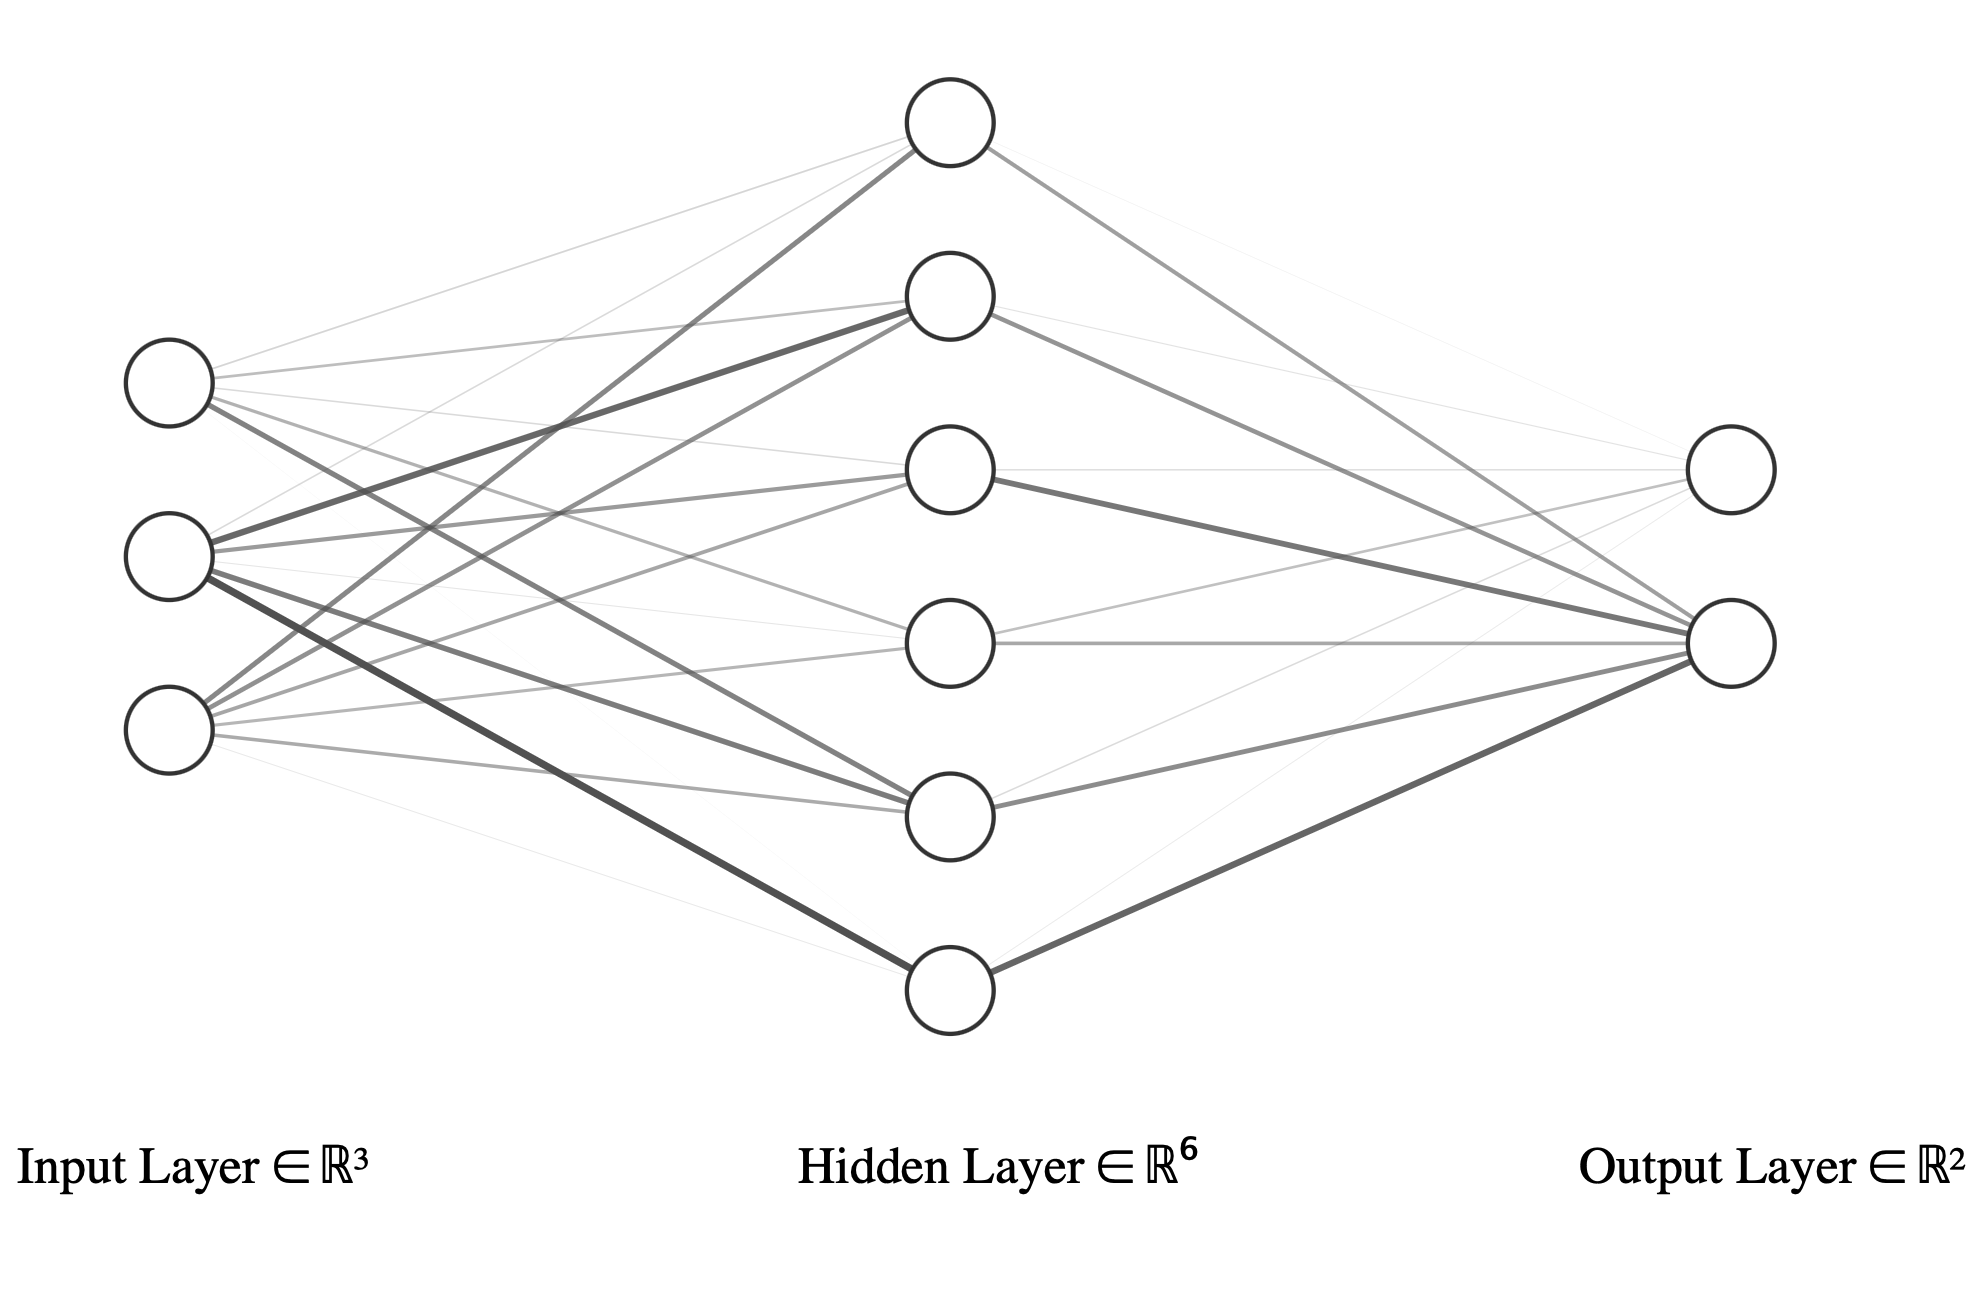
\includegraphics[scale=0.3]{Figures/mlp.png}
\caption{Representation of a simple MLP}
\label{mlp}
\end{figure}

An MLP is a function of several parameters and hyper-parameters. The parameters of the MLP are the weights $\theta$ of each connection, and the hyper-parameters are:
\begin{itemize}
	\item The number of hidden layers
	\item The number of neurons per layer
	\item The weights initialisation values
	\item The activation functions of each layer
	\item The learning rate $\alpha$
	\item The number of epochs $N$
	\item The loss function for backpropagation
\end{itemize}

The training process is relatively straightforward and consists of tuning the values of the weights for $N$ epochs (\cite{mlptraining}). Each epoch goes through several cycles of forward and back propagations over a subset of the training set: the network output is calculated using the weights and activation functions (forward propagation). This output is compared to the expected output using the loss function. The weight values are then updated using the loss function, starting from the output layer and moving back toward the input layer (backpropagation).


The Deep Q-Learning (Subsection \ref{dqlearningsection}) and the DDPG (Subsection \ref{ddpgsection}) algorithms that we introduced previously are implemented using NNs. In the case of autonomous racing using LiDAR data, the input layer could have as many neurons as there are LiDAR points. The output layer would only have two neurons: one returning the steering angle (maybe a value $\theta \in [-\pi,\pi]$, with $\theta$ in radians) and the other returning the motors command $m \in [0,1]$ for example.


\subsection{Convolutional Neural Networks}

Convolutional Neural Networks are a type of NNs better suited to handle 2 or 3-dimensional data (\cite{cnnintro}). The problem with using simple MLP for such data is that the NN loses all the spatial structure of the image with $h \times w$ pixels into a 1D array of $h \times w$ values. CNNs can preserve the spatial relationship between the pixels and let the NN learn the internal features of the data by using three main types of layers: convolutional, pooling and fully connected layers; an example is given in Figure \ref{cnnex}. \newline
The convolutional layer is defined by the filters, the feature maps, the stride and the padding. The filters correspond to the ``neurons": they have input weights and output a value. For a 2D image, the filter is a square of a specific size (Figure \ref{conv2D}).

\begin{figure}[H]
\centering
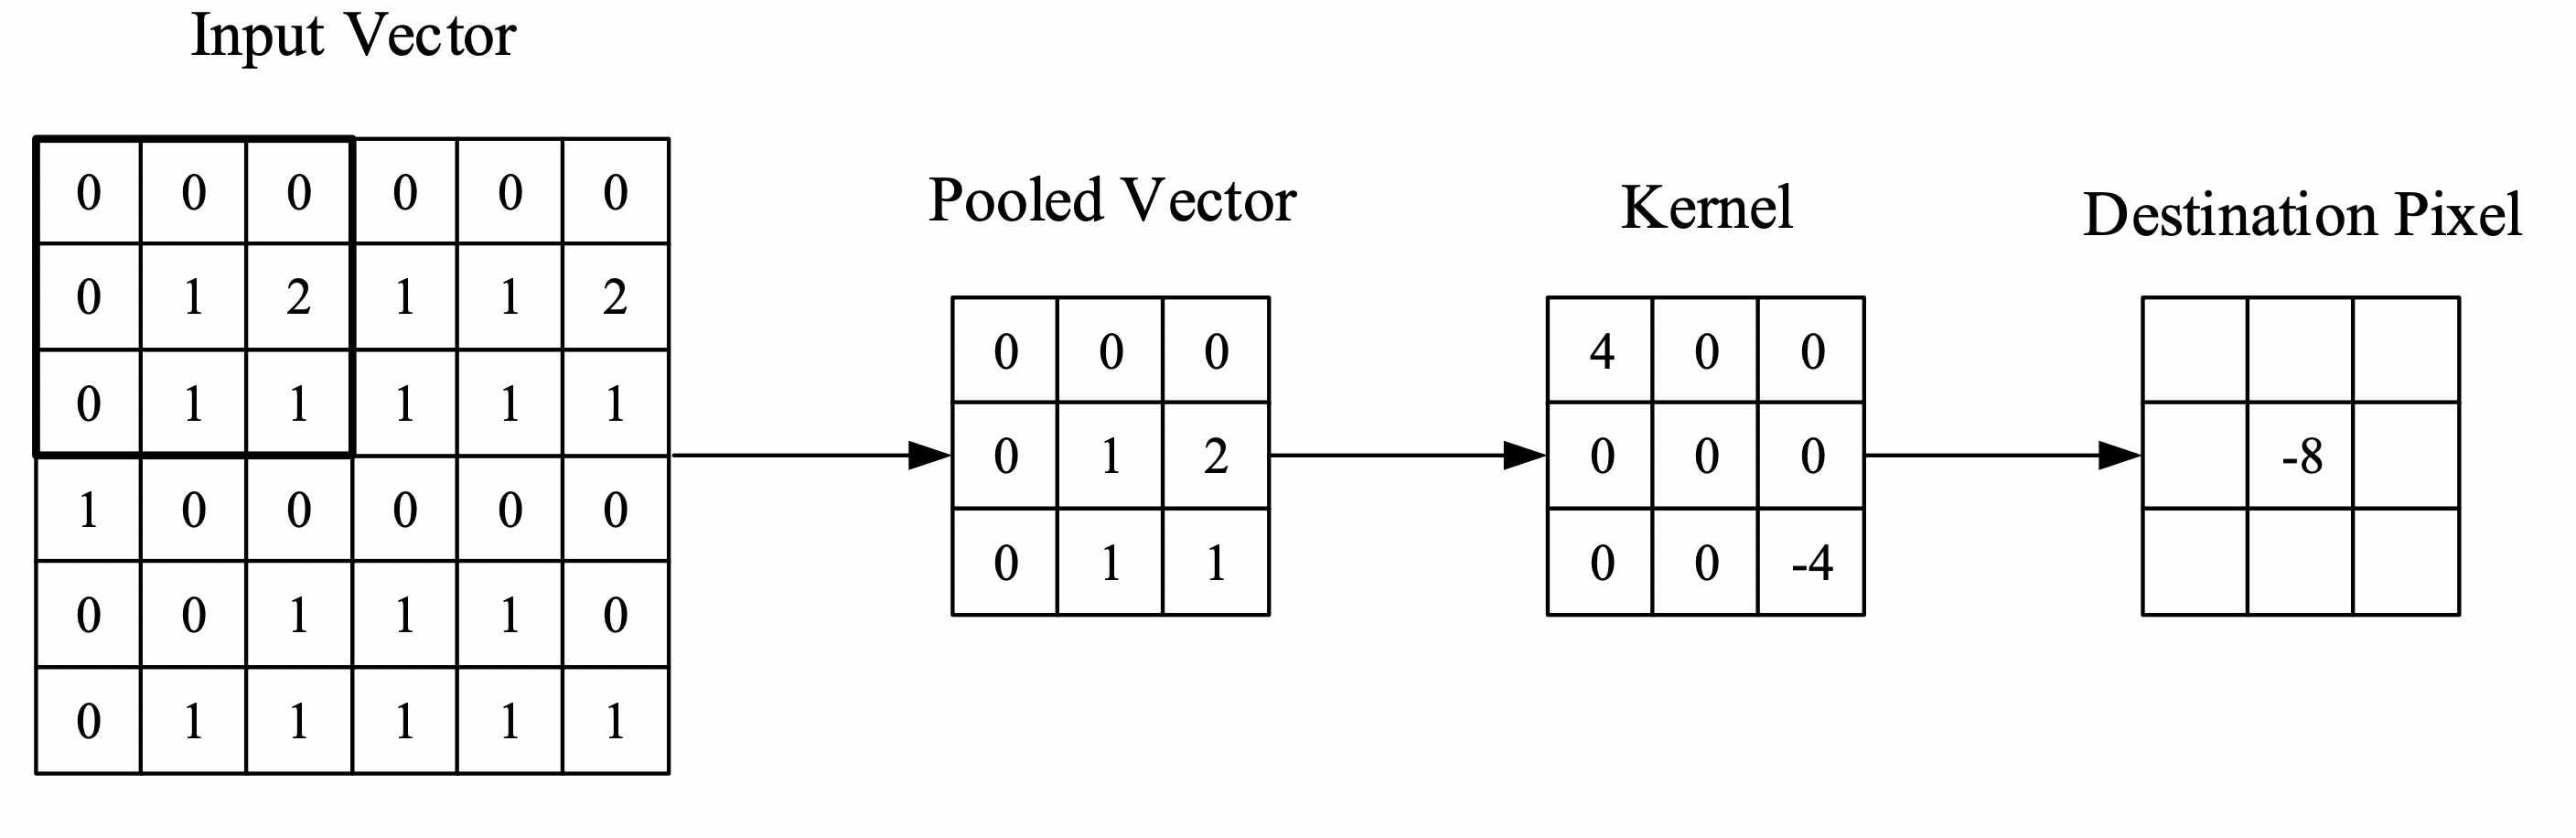
\includegraphics[scale=0.3]{Figures/conv2D.png}
\caption{Example of a Convolutional Neural Network, taken from \cite{cnnintro}}
\label{conv2D}
\end{figure}


The feature map is the output of a filter applied to the previous layer of the network. When the filter is moved across the input data, it returns different values that are added to the feature map; the amount by which the filter is moved is the stride, and padding can be added to the border of the input if the filter doesn't perfectly ``line-up" with the input. The size of the feature map is a function of the input size (height, width and depth) $v$, the size of the filter $f$, the amount of padding added $p$ and the stride $s$ such as (Equation \ref{convequ}):

\begin{equation}
\label{convequ}
	\text{Output size} = \frac{(v-s)+2p}{s+1}
\end{equation}

The convolutional layer is thus a great way of reducing the input size while preserving the spatial relationship. \newline
The pooling layer aims to reduce the dimensionality of the data slowly. The filter of size $f$ moves across the input data with a stride $s$ and outputs the max value (for max-pooling) of its area $s \times s$. It thus scales down the size of the input data into something more manageable. Because data is lost in the process, the size of the filter should be kept to $2 \times 2$ or $3 \times 3$.\newline
Finally, the fully connected layer of a CNN corresponds to an MLP as defined in Subsection \ref{mlpsection}.

\begin{figure}[H]
\centering
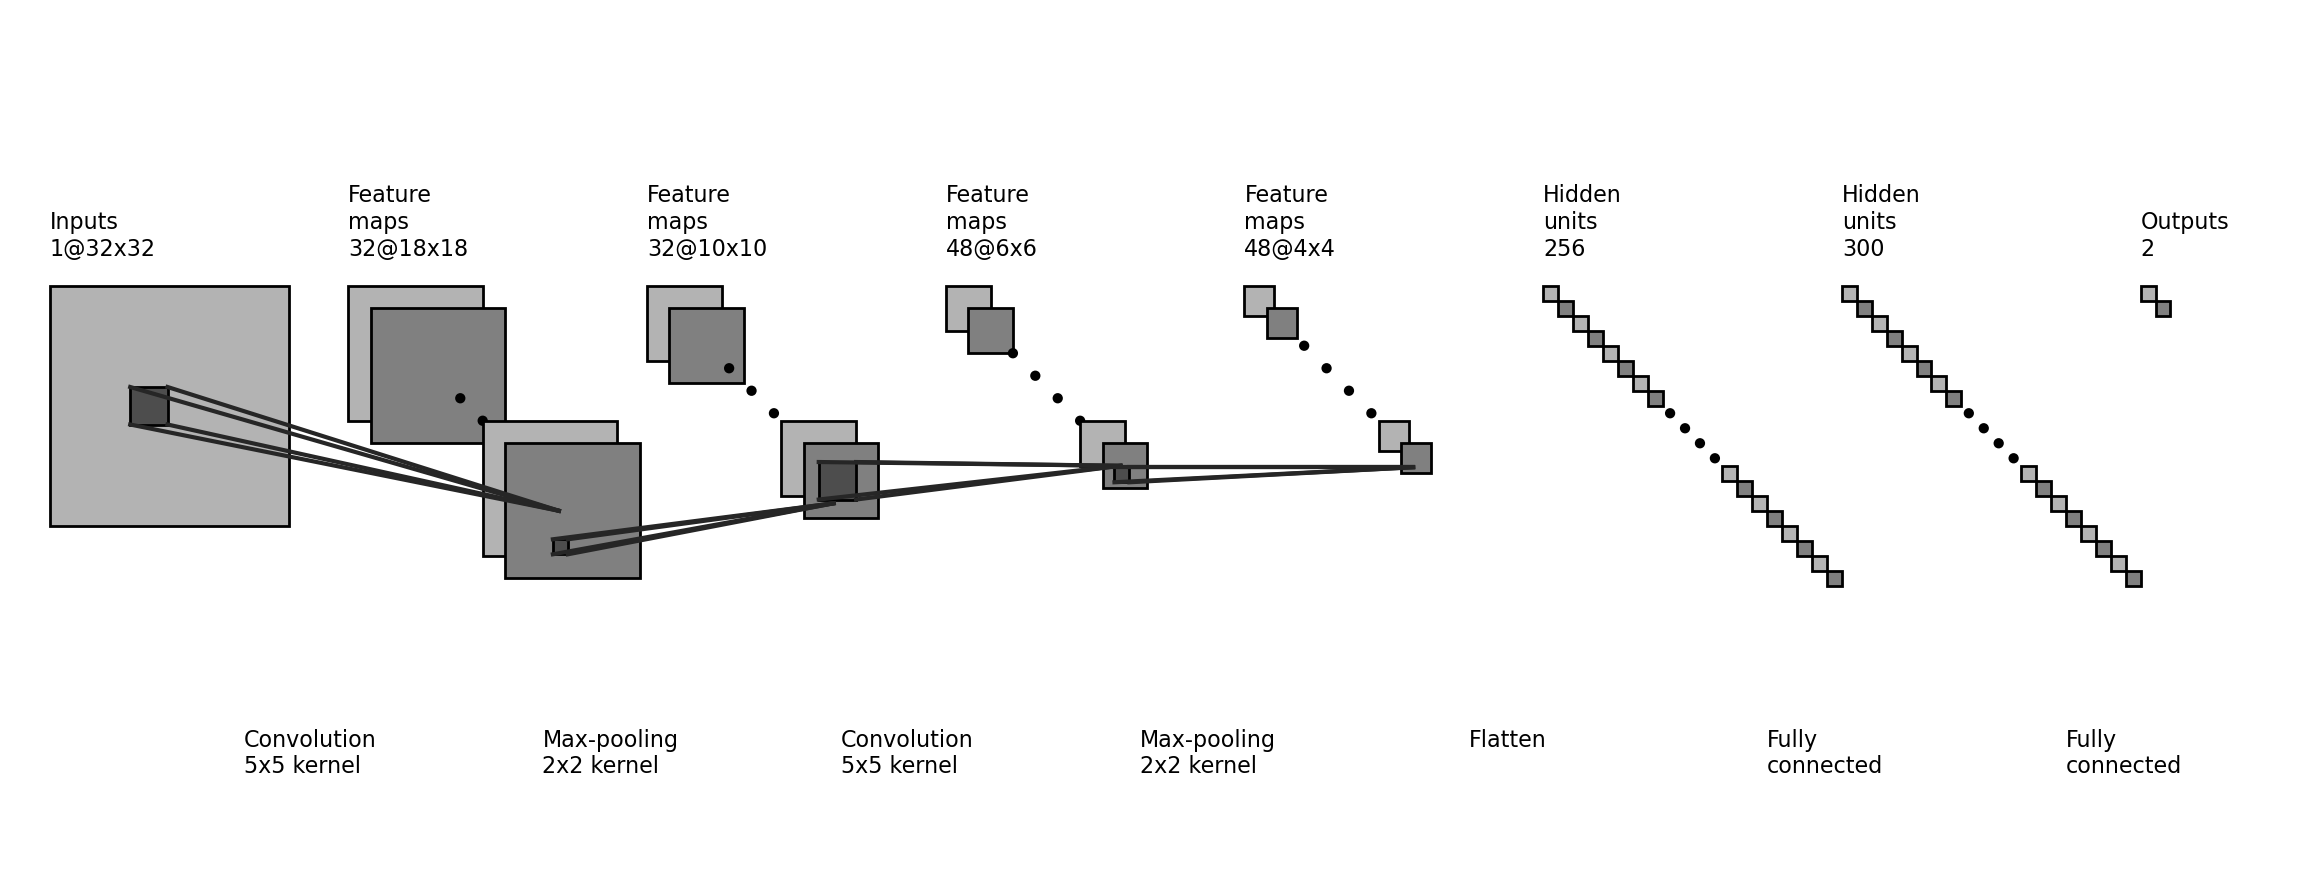
\includegraphics[scale=0.184]{Figures/cnn.png}
\caption{Example of a Convolutional Neural Network, made using \\ \url{http://alexlenail.me/NN-SVG/LeNet.html}}
\label{cnnex}
\end{figure}

In this example, the 2D input data goes through a max-pooling layer, a convolutional layer, another max-pooling layer, then gets flattened and goes through a fully connected network with an input layer of size 256, a hidden layer of size 300 and an output layer of size 2 (corresponding to steering and motors signals). \newline
In the case of using LiDAR data for a racing car controller, CNNs are shown to generally offer better results (\cite{bosello}): we will try to replicate those results and confirm that CNNs are superior when used with the controllers we will implement. We will implement fully connected NNs and CNNs to parse the LiDAR data feed after some pre-processing; more information about technical details is given in Chapter \ref{Chapter3}.

\section{Robot Operating System and F1Tenth System}
\label{rosandf1tenth}
\subsection{ROS framework}

Robotics has long been a playground for Reinforcement Learning algorithms (\cite{rlintro}), and many implementations of those algorithms have been done using Robot Operating System (ROS). ROS is a robotic software platform that is open-source (BSD license) and provides a vast amount of services, tools and libraries to serve as the framework of any robotic platform. Because ROS is open-source, it is straightforward to contribute to the project, and many users have developed and shared their own libraries. ROS is also a meta-operating system, meaning it behaves like an operating system but runs on a Unix-based OS. The goal of ROS is to enable code sharing and collaboration among coders: ROS was thus designed as a distributed framework of processes called nodes that can be grouped in packages and stacks to be shared easily. A package is the smallest self-functioning unit that exists in ROS. Most ROS projects contain several packages that build up on each other and are declared as \textit{dependancies} of each other. Packages are located inside a catkin workspace, built using the catkin build system with the command \verb |catkin_make|. Catkin is the official build system of ROS and was designed to replace rosbuild. A catkin workspace containing packages has the following general structure (Figure \ref{rosdirectory}):

\begin{figure}[H]
\centering
\begin{forest}
  for tree={
    font=\ttfamily,
    grow'=0,
    child anchor=west,
    parent anchor=south,
    anchor=west,
    calign=first,
    edge path={
      \noexpand\path [draw, \forestoption{edge}]
      (!u.south west) +(7.5pt,0) |- node[fill,inner sep=1.25pt] {} (.child anchor)\forestoption{edge label};
    },
    before typesetting nodes={
      if n=1
        {insert before={[,phantom]}}
        {}
    },
    fit=band,
    before computing xy={l=15pt},
  }
[/$\sim$ workspace/
  [build/]
  [devel/]
    [src/
      [CMakeLists.txt]
      [package1/
      	[include/]
      	[msg/]
      	[srv/]
      	[launch/]
      	[src/
      		[node1.cpp]
      	]
      	[CMakeLists.txt]
      	[package.xml]
      ]
  	]
  ]
]
\end{forest}
\caption{Directory structure of a ROS workspace}
\label{rosdirectory}
\end{figure}


Each package has to have the \verb |CMakeList.txt| and the \verb |package.txt| files. The \verb |CMakeList.txt| tells catkin how to compile the package, with the locations of the different libraries and subdirectories. The \verb |package.xml| contains several elements, including the dependencies (other packages) used by the package, the name and a description of the package, the tools used to build the package and nodelets, which are external tools for the package. The package architecture is, however, not a rigid as the workspace architecture, the source folder can be renamed, and some nodes can be put in other packages.
\newline
The architecture of a ROS package can be represented as a graph, with nodes connected by edges that are called \textit{topics} (Figure \ref{ros}). Each node can send and receive messages to other nodes using the topics. The primary process in this graph is called the \textit{ROS Master}. It registers all the nodes and sets up the node-to-node communications for each topic. A ROS program is decentralised because the messages and service calls don't go through the ROS Master; they are all peer-to-peer communications. This is a very modular architecture that works very well when robots themselves are made of several modules communicating with each other.

\begin{figure}[H]
\centering
\tikzset{every picture/.style={line width=0.75pt}} %set default line width to 0.75pt        

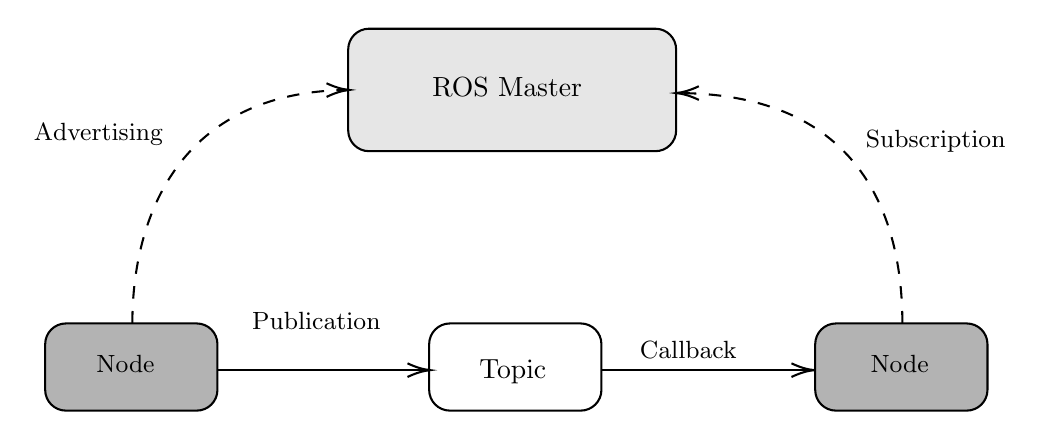
\begin{tikzpicture}[x=0.75pt,y=0.75pt,yscale=-1,xscale=1]
%uncomment if require: \path (0,300); %set diagram left start at 0, and has height of 300

%Shape: Rectangle [id:dp4384866938999734] 
\draw  [fill={rgb, 255:red, 230; green, 230; blue, 230 }  ,fill opacity=1 ] (243,73) .. controls (243,67.48) and (247.48,63) .. (253,63) -- (391,63) .. controls (396.52,63) and (401,67.48) .. (401,73) -- (401,112) .. controls (401,117.52) and (396.52,122) .. (391,122) -- (253,122) .. controls (247.48,122) and (243,117.52) .. (243,112) -- cycle ;
%Shape: Rectangle [id:dp8543292300869088] 
\draw   (282,215) .. controls (282,209.48) and (286.48,205) .. (292,205) -- (355,205) .. controls (360.52,205) and (365,209.48) .. (365,215) -- (365,237) .. controls (365,242.52) and (360.52,247) .. (355,247) -- (292,247) .. controls (286.48,247) and (282,242.52) .. (282,237) -- cycle ;
%Shape: Rectangle [id:dp0036299673216855233] 
\draw  [fill={rgb, 255:red, 179; green, 179; blue, 179 }  ,fill opacity=1 ] (97,215) .. controls (97,209.48) and (101.48,205) .. (107,205) -- (170,205) .. controls (175.52,205) and (180,209.48) .. (180,215) -- (180,237) .. controls (180,242.52) and (175.52,247) .. (170,247) -- (107,247) .. controls (101.48,247) and (97,242.52) .. (97,237) -- cycle ;
%Straight Lines [id:da6462256681950369] 
\draw    (180.17,227.5) -- (280.5,227.5) ;
\draw [shift={(282.5,227.5)}, rotate = 180] [color={rgb, 255:red, 0; green, 0; blue, 0 }  ][line width=0.75]    (10.93,-3.29) .. controls (6.95,-1.4) and (3.31,-0.3) .. (0,0) .. controls (3.31,0.3) and (6.95,1.4) .. (10.93,3.29)   ;
%Straight Lines [id:da6599201831964536] 
\draw    (365.17,227.5) -- (465.5,227.5) ;
\draw [shift={(467.5,227.5)}, rotate = 180] [color={rgb, 255:red, 0; green, 0; blue, 0 }  ][line width=0.75]    (10.93,-3.29) .. controls (6.95,-1.4) and (3.31,-0.3) .. (0,0) .. controls (3.31,0.3) and (6.95,1.4) .. (10.93,3.29)   ;
%Shape: Rectangle [id:dp7953194571282391] 
\draw  [fill={rgb, 255:red, 179; green, 179; blue, 179 }  ,fill opacity=1 ] (468,215) .. controls (468,209.48) and (472.48,205) .. (478,205) -- (541,205) .. controls (546.52,205) and (551,209.48) .. (551,215) -- (551,237) .. controls (551,242.52) and (546.52,247) .. (541,247) -- (478,247) .. controls (472.48,247) and (468,242.52) .. (468,237) -- cycle ;
%Curve Lines [id:da8155840447764608] 
\draw  [dash pattern={on 4.5pt off 4.5pt}]  (139,205) .. controls (139,153.26) and (161.77,93.6) .. (242.28,92.51) ;
\draw [shift={(243.5,92.5)}, rotate = 179.65] [color={rgb, 255:red, 0; green, 0; blue, 0 }  ][line width=0.75]    (10.93,-3.29) .. controls (6.95,-1.4) and (3.31,-0.3) .. (0,0) .. controls (3.31,0.3) and (6.95,1.4) .. (10.93,3.29)   ;
%Curve Lines [id:da5232732353300578] 
\draw  [dash pattern={on 4.5pt off 4.5pt}]  (510,205) .. controls (510,153.26) and (489.7,94.59) .. (402.32,94) ;
\draw [shift={(401,94)}, rotate = 360] [color={rgb, 255:red, 0; green, 0; blue, 0 }  ][line width=0.75]    (10.93,-3.29) .. controls (6.95,-1.4) and (3.31,-0.3) .. (0,0) .. controls (3.31,0.3) and (6.95,1.4) .. (10.93,3.29)   ;

% Text Node
\draw (282,85) node [anchor=north west][inner sep=0.75pt]   [align=left] {ROS Master};
% Text Node
\draw (304.7,221) node [anchor=north west][inner sep=0.75pt]   [align=left] {Topic};
% Text Node
\draw (120.15,219) node [anchor=north west][inner sep=0.75pt]  [font=\small] [align=left] {Node};
% Text Node
\draw (195.07,198) node [anchor=north west][inner sep=0.75pt]  [font=\small] [align=left] {\begin{minipage}[lt]{46.61pt}\setlength\topsep{0pt}
\begin{center}
Publication
\end{center}

\end{minipage}};
% Text Node
\draw (380.07,212) node [anchor=north west][inner sep=0.75pt]  [font=\small] [align=left] {\begin{minipage}[lt]{37.93pt}\setlength\topsep{0pt}
\begin{center}
Callback
\end{center}

\end{minipage}};
% Text Node
\draw (493.15,219) node [anchor=north west][inner sep=0.75pt]  [font=\small] [align=left] {Node};
% Text Node
\draw (89.07,107.19) node [anchor=north west][inner sep=0.75pt]  [font=\small] [align=left] {\begin{minipage}[lt]{48.14pt}\setlength\topsep{0pt}
\begin{center}
Advertising
\end{center}
\end{minipage}};
% Text Node
\draw (489.07,110.19) node [anchor=north west][inner sep=0.75pt]  [font=\small] [align=left] {\begin{minipage}[lt]{53.24pt}\setlength\topsep{0pt}
\begin{center}
Subscription
\end{center}
\end{minipage}};
\end{tikzpicture}
\caption{ROS nodes interactions}
\label{ros}
\end{figure}

A ROS node is a process running as part of the ROS graph, written either in Python or C++. They all have a name that must be registered with the ROS Master and represent most of the code written for a ROS project. To send a message to a topic, a node has to register as a publisher; to receive messages, it has to register as a subscriber. The messages themselves can be any type of data: in the case of the F1Tenth system, they will contain sensor data with the LiDAR points, the actuators commands for the steering and the motor control commands for the speed.


\subsection{F1Tenth framework}

The F1Tenth platform was designed as a teaching and open-source research tool and, as such, is perfect for this project. It consists of a small racing car composed of a lower and upper chassis with a 5000 mAh battery and several autonomy elements: a WiFi antenna, a UST-10LX LiDAR, an NVIDIA Jetson as the Electronic Control Unit (ECU), an NVIDIA Jetson NX GPU for parallel computing, a speed controller and a power board. \newline
The main interest of the F1Tenth car is that it offers hardware and software similar to full-scale racing systems: realistic dynamics, with Ackermann steering and high maximum speed. The idea of Ackermann steering is simple: in a corner, the inner front wheel has a larger turning angle than the outer front wheel so that the tires are not slipping sideways. \newline 
The F1Tenth simulator used for this project is the default one: developed as a lightweight 2D simulator built using ROS, it is written in C++ and displays 3D graphics using RViz. RViz is a three-dimensional visualiser used to see how a robot evolves in its environment. Like most ROS tools, it is highly modular, with several different types of visualisations. The F1Tenth simulator simulates the car motion and collisions, handles the publishing of LiDAR scans and odometry data and is built for the fast prototyping of racing algorithms, which corresponds perfectly to this MSc project. The basic ROS architecture of the simulator is presented in Figure \ref{f1tenth}. Another possibility would have been to develop our own simulator, but this would have been too time-consuming. The default simulator is good enough for our needs; however, it does not support more than one car; this could be a problem later if we want to test our algorithms in a multi-car racing environment.

\begin{figure}[H]
\centering
\tikzset{every picture/.style={line width=0.75pt}} %set default line width to 0.75pt        

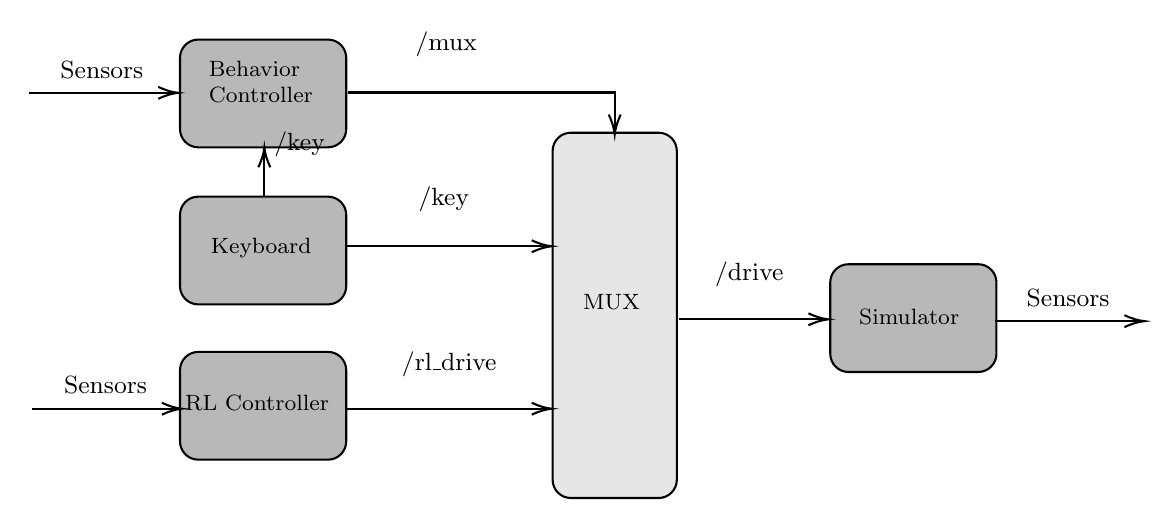
\begin{tikzpicture}[x=0.66pt,y=0.66pt,yscale=-1,xscale=1]
%uncomment if require: \path (0,300); %set diagram left start at 0, and has height of 300

%Shape: Rectangle [id:dp2579715088062431] 
\draw  [fill={rgb, 255:red, 230; green, 230; blue, 230 }  ,fill opacity=1 ] (310,85) .. controls (310,79.48) and (314.48,75) .. (320,75) -- (368,75) .. controls (373.52,75) and (378,79.48) .. (378,85) -- (378,265) .. controls (378,270.52) and (373.52,275) .. (368,275) -- (320,275) .. controls (314.48,275) and (310,270.52) .. (310,265) -- cycle ;
%Shape: Rectangle [id:dp9236936454384124] 
\draw  [fill={rgb, 255:red, 184; green, 184; blue, 184 }  ,fill opacity=1 ] (462,157) .. controls (462,151.48) and (466.48,147) .. (472,147) -- (543,147) .. controls (548.52,147) and (553,151.48) .. (553,157) -- (553,196) .. controls (553,201.52) and (548.52,206) .. (543,206) -- (472,206) .. controls (466.48,206) and (462,201.52) .. (462,196) -- cycle ;
%Straight Lines [id:da04665976383851422] 
\draw    (379.17,177.17) -- (459,177.17) ;
\draw [shift={(461,177.17)}, rotate = 180] [color={rgb, 255:red, 0; green, 0; blue, 0 }  ][line width=0.75]    (10.93,-3.29) .. controls (6.95,-1.4) and (3.31,-0.3) .. (0,0) .. controls (3.31,0.3) and (6.95,1.4) .. (10.93,3.29)   ;
%Straight Lines [id:da7993604456864187] 
\draw    (552.17,178.17) -- (632,178.17) ;
\draw [shift={(634,178.17)}, rotate = 180] [color={rgb, 255:red, 0; green, 0; blue, 0 }  ][line width=0.75]    (10.93,-3.29) .. controls (6.95,-1.4) and (3.31,-0.3) .. (0,0) .. controls (3.31,0.3) and (6.95,1.4) .. (10.93,3.29)   ;
%Shape: Rectangle [id:dp4290310775587869] 
\draw  [fill={rgb, 255:red, 184; green, 184; blue, 184 }  ,fill opacity=1 ] (106,34) .. controls (106,28.48) and (110.48,24) .. (116,24) -- (187,24) .. controls (192.52,24) and (197,28.48) .. (197,34) -- (197,73) .. controls (197,78.52) and (192.52,83) .. (187,83) -- (116,83) .. controls (110.48,83) and (106,78.52) .. (106,73) -- cycle ;
%Straight Lines [id:da3636958296734685] 
\draw    (198,53) -- (344,53) -- (344,74) ;
\draw [shift={(344,76)}, rotate = 270] [color={rgb, 255:red, 0; green, 0; blue, 0 }  ][line width=0.75]    (10.93,-3.29) .. controls (6.95,-1.4) and (3.31,-0.3) .. (0,0) .. controls (3.31,0.3) and (6.95,1.4) .. (10.93,3.29)   ;
%Straight Lines [id:da14979101244440018] 
\draw    (23.17,53.17) -- (103,53.17) ;
\draw [shift={(105,53.17)}, rotate = 180] [color={rgb, 255:red, 0; green, 0; blue, 0 }  ][line width=0.75]    (10.93,-3.29) .. controls (6.95,-1.4) and (3.31,-0.3) .. (0,0) .. controls (3.31,0.3) and (6.95,1.4) .. (10.93,3.29)   ;
%Shape: Rectangle [id:dp6150892713225873] 
\draw  [fill={rgb, 255:red, 184; green, 184; blue, 184 }  ,fill opacity=1 ] (106,120) .. controls (106,114.48) and (110.48,110) .. (116,110) -- (187,110) .. controls (192.52,110) and (197,114.48) .. (197,120) -- (197,159) .. controls (197,164.52) and (192.52,169) .. (187,169) -- (116,169) .. controls (110.48,169) and (106,164.52) .. (106,159) -- cycle ;
%Straight Lines [id:da37495512013154664] 
\draw    (152.17,110.17) -- (152.17,85) ;
\draw [shift={(152.17,83)}, rotate = 90] [color={rgb, 255:red, 0; green, 0; blue, 0 }  ][line width=0.75]    (10.93,-3.29) .. controls (6.95,-1.4) and (3.31,-0.3) .. (0,0) .. controls (3.31,0.3) and (6.95,1.4) .. (10.93,3.29)   ;
%Straight Lines [id:da5143374143030996] 
\draw    (197,137.17) -- (307.5,137.17) ;
\draw [shift={(309.5,137.17)}, rotate = 180] [color={rgb, 255:red, 0; green, 0; blue, 0 }  ][line width=0.75]    (10.93,-3.29) .. controls (6.95,-1.4) and (3.31,-0.3) .. (0,0) .. controls (3.31,0.3) and (6.95,1.4) .. (10.93,3.29)   ;
%Shape: Rectangle [id:dp2649593712992906] 
\draw  [fill={rgb, 255:red, 184; green, 184; blue, 184 }  ,fill opacity=1 ] (106,205) .. controls (106,199.48) and (110.48,195) .. (116,195) -- (187,195) .. controls (192.52,195) and (197,199.48) .. (197,205) -- (197,244) .. controls (197,249.52) and (192.52,254) .. (187,254) -- (116,254) .. controls (110.48,254) and (106,249.52) .. (106,244) -- cycle ;
%Straight Lines [id:da47062201276435833] 
\draw    (25.17,226.11) -- (105,226.11) ;
\draw [shift={(107,226.11)}, rotate = 180] [color={rgb, 255:red, 0; green, 0; blue, 0 }  ][line width=0.75]    (10.93,-3.29) .. controls (6.95,-1.4) and (3.31,-0.3) .. (0,0) .. controls (3.31,0.3) and (6.95,1.4) .. (10.93,3.29)   ;
%Straight Lines [id:da9654740651191391] 
\draw    (197.17,226.11) -- (307.5,226.11) ;
\draw [shift={(309.5,226.11)}, rotate = 180] [color={rgb, 255:red, 0; green, 0; blue, 0 }  ][line width=0.75]    (10.93,-3.29) .. controls (6.95,-1.4) and (3.31,-0.3) .. (0,0) .. controls (3.31,0.3) and (6.95,1.4) .. (10.93,3.29)   ;

% Text Node
\draw (325,162) node [anchor=north west][inner sep=0.75pt] [font=\footnotesize]  [align=left] {MUX};
% Text Node
\draw (476.15,170) node [anchor=north west][inner sep=0.75pt] [font=\footnotesize] [align=left] {Simulator};
% Text Node
\draw (396.94,144.06) node [anchor=north west][inner sep=0.75pt]  [font=\small] [align=left] {\begin{minipage}[lt]{25.17pt}\setlength\topsep{0pt}
\begin{center}
/drive
\end{center}

\end{minipage}};
% Text Node
\draw (562.94,159.06) node [anchor=north west][inner sep=0.75pt]  [font=\small] [align=left] {\begin{minipage}[lt]{36.4pt}\setlength\topsep{0pt}
\begin{center}
Sensors
\end{center}

\end{minipage}};
% Text Node
\draw (120.15,34) node [anchor=north west][inner sep=0.75pt]  [font=\footnotesize] [align=left] {Behavior\\Controller};
% Text Node
\draw (232.94,18.06) node [anchor=north west][inner sep=0.75pt]  [font=\small] [align=left] {\begin{minipage}[lt]{22.62pt}\setlength\topsep{0pt}
\begin{center}
/mux
\end{center}

\end{minipage}};
% Text Node
\draw (33.94,34.06) node [anchor=north west][inner sep=0.75pt]  [font=\small] [align=left] {\begin{minipage}[lt]{36.4pt}\setlength\topsep{0pt}
\begin{center}
Sensors
\end{center}

\end{minipage}};
% Text Node
\draw (121.15,131) node [anchor=north west][inner sep=0.75pt]  [font=\footnotesize] [align=left] {Keyboard};
% Text Node
\draw (154.94,73) node [anchor=north west][inner sep=0.75pt]  [font=\small] [align=left] {\begin{minipage}[lt]{19.56pt}\setlength\topsep{0pt}
\begin{center}
/key
\end{center}

\end{minipage}};
% Text Node
\draw (233.94,103) node [anchor=north west][inner sep=0.75pt]  [font=\small] [align=left] {\begin{minipage}[lt]{19.56pt}\setlength\topsep{0pt}
\begin{center}
/key
\end{center}

\end{minipage}};
% Text Node
\draw (107.15,217) node [anchor=north west][inner sep=0.75pt]  [font=\footnotesize] [align=left] {RL Controller};
% Text Node
\draw (35.94,207) node [anchor=north west][inner sep=0.75pt]  [font=\small] [align=left] {\begin{minipage}[lt]{36.4pt}\setlength\topsep{0pt}
\begin{center}
Sensors
\end{center}

\end{minipage}};
% Text Node
\draw (224.94,193) node [anchor=north west][inner sep=0.75pt]  [font=\small] [align=left] {\begin{minipage}[lt]{35.37pt}\setlength\topsep{0pt}
\begin{center}
/rl\_drive
\end{center}
\end{minipage}};
\end{tikzpicture}
\caption{F1Tenth system architecture}
\label{f1tenth}
\end{figure}

The simulator was developed to be interchangeable with the actual car system. Once the training of the RL controller has been finished in the simulator, the simulator node can be replaced by the F1Tenth car itself, and if the topics' names are not changed, then the same code can be used to drive the car to evaluate the sim-2-real gap. This way, we can easily swap between different types of RL controllers, both in the simulator and on the actual car. The \verb |MUX| node listens to the \verb |/mux| topic to know which controller is on; in our case, it would be the \verb |RL Controller| one, so \verb |MUX| listens to \verb |rl_drive| and then transmits the message to \verb |/drive|. Then either the \verb |Simulator| node or the car itself listens to the \verb |/drive| topic, and the state of the car gets updated. In the simulator, once a training epoch is completed, or once the car hits a wall, we can move it back to the start of the race track by publishing a Pose message to the \verb |/pose| topic.


\subsection{Wall Following controller for the F1Tenth platform}

During the project, we will implement a Wall Following controller to be compared against RL methods. Unlike the RL controllers introduced in the previous sections, the Wall Following controller is not an ML algorithm; it relies on a Proportional-Integral-Derivative controller to maintain the desired distance with one of the walls of the race track. The challenge with this method is to measure the distance to the wall and anticipate the car's trajectory. To determine the distance of the car to the wall, 2 LiDAR measurements, $l_1$ and $l_2$ are made (Figure \ref{walllidar}). The first measurement is perpendicular to the car's direction (angle of 0°), the second at an angle $0 < \theta < 90°$. Using trigonometry, the angle $\alpha$ between the direction of the car and the wall can be expressed as Equation \ref{eqalpha}:

\begin{equation}
\label{eqalpha}
\alpha = \arctan \left(\frac{l_1 \cos(\theta) - l_2}{l_1 \sin(\theta)}\right)
\end{equation}

$D_t$ can then be expressed as $D_t = l_2 \cos(\alpha)$.

\begin{figure}[H]
\centering
\tikzset{every picture/.style={line width=0.75pt}} %set default line width to 0.75pt        
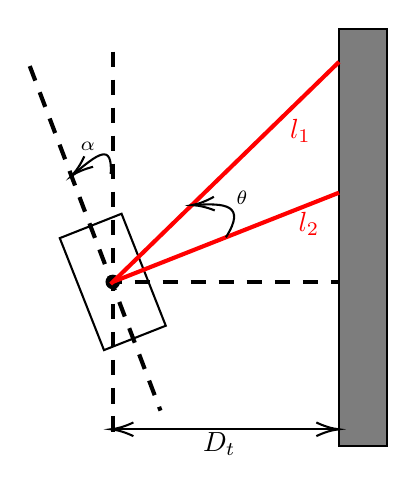
\begin{tikzpicture}[x=0.75pt,y=0.75pt,yscale=-1,xscale=1]
%uncomment if require: \path (0,300); %set diagram left start at 0, and has height of 300

%Shape: Rectangle [id:dp4311350167300596] 
\draw  [fill={rgb, 255:red, 125; green, 125; blue, 125 }  ,fill opacity=1 ] (357,49) -- (380,49) -- (380,250) -- (357,250) -- cycle ;
%Shape: Rectangle [id:dp7782596183463344] 
\draw   (222.47,149.9) -- (252.23,138.15) -- (273.53,192.1) -- (243.77,203.85) -- cycle ;
%Shape: Circle [id:dp5936067004712828] 
\draw  [fill={rgb, 255:red, 0; green, 0; blue, 0 }  ,fill opacity=1 ] (245,171) .. controls (245,169.34) and (246.34,168) .. (248,168) .. controls (249.66,168) and (251,169.34) .. (251,171) .. controls (251,172.66) and (249.66,174) .. (248,174) .. controls (246.34,174) and (245,172.66) .. (245,171) -- cycle ;
%Straight Lines [id:da6106744350332936] 
\draw [line width=1.5]  [dash pattern={on 5.63pt off 4.5pt}]  (245,171) -- (357,171) ;
%Straight Lines [id:da2725245856447387] 
\draw [line width=1.5]  [dash pattern={on 5.63pt off 4.5pt}]  (248,60) -- (248,249) ;
%Straight Lines [id:da01842142719484019] 
\draw    (249,242) -- (355,242) ;
\draw [shift={(357,242)}, rotate = 180] [color={rgb, 255:red, 0; green, 0; blue, 0 }  ][line width=0.75]    (10.93,-3.29) .. controls (6.95,-1.4) and (3.31,-0.3) .. (0,0) .. controls (3.31,0.3) and (6.95,1.4) .. (10.93,3.29)   ;
\draw [shift={(247,242)}, rotate = 0] [color={rgb, 255:red, 0; green, 0; blue, 0 }  ][line width=0.75]    (10.93,-3.29) .. controls (6.95,-1.4) and (3.31,-0.3) .. (0,0) .. controls (3.31,0.3) and (6.95,1.4) .. (10.93,3.29)   ;
%Straight Lines [id:da1822654047018304] 
\draw [line width=1.5]  [dash pattern={on 5.63pt off 4.5pt}]  (208,67) -- (271,233) ;
%Curve Lines [id:da2922120325109894] 
\draw    (247,119) .. controls (247.96,103.64) and (240.63,109.48) .. (229.42,118.82) ;
\draw [shift={(228,120)}, rotate = 320.19] [color={rgb, 255:red, 0; green, 0; blue, 0 }  ][line width=0.75]    (10.93,-3.29) .. controls (6.95,-1.4) and (3.31,-0.3) .. (0,0) .. controls (3.31,0.3) and (6.95,1.4) .. (10.93,3.29)   ;
%Straight Lines [id:da6331858332787972] 
\draw [color={rgb, 255:red, 255; green, 0; blue, 0 }  ,draw opacity=1 ][line width=1.5]    (248,171) -- (357,128) ;
%Straight Lines [id:da021082029935662883] 
\draw [color={rgb, 255:red, 255; green, 0; blue, 0 }  ,draw opacity=1 ][line width=1.5]    (247,172) -- (357,65) ;
%Curve Lines [id:da9871331844967834] 
\draw    (302.5,149.5) .. controls (312.58,133.66) and (301.92,133.03) .. (287.78,133.89) ;
\draw [shift={(286,134)}, rotate = 356.19] [color={rgb, 255:red, 0; green, 0; blue, 0 }  ][line width=0.75]    (10.93,-3.29) .. controls (6.95,-1.4) and (3.31,-0.3) .. (0,0) .. controls (3.31,0.3) and (6.95,1.4) .. (10.93,3.29)   ;
% Text Node
\draw (290,242) node [anchor=north west][inner sep=0.75pt]    {$D_{t}$};
% Text Node
\draw (231,102) node [anchor=north west][inner sep=0.75pt]  [font=\scriptsize] [align=left] {$\alpha$};
% Text Node
\draw (306,125.5) node [anchor=north west][inner sep=0.75pt]  [font=\scriptsize] [align=left] {$\theta$};
% Text Node
\draw (336,136) node [anchor=north west][inner sep=0.75pt] {${\textstyle \textcolor[rgb]{1,0,0}{l_{2}}}$};;
% Text Node
\draw (332,91) node [anchor=north west][inner sep=0.75pt]    {${\textstyle \textcolor[rgb]{1,0,0}{l_{1}}}$};
\end{tikzpicture}
\caption{Wall Following geometry}
\label{walllidar}
\end{figure}

However, as explained in \cite{wallfollowcourse}, if we use the car's current position, the controller may not be able to respond fast enough to account for the computational delay, and the car's trajectory may not be optimal. Instead, the car's position at time step $t+1$ is used (Equation \ref{eqalpha2}), with $D_{t+1}$ the car's position at time step $t+1$, $\Delta t $ the duration of a time step and $v_t$ the speed of the car at time step $t$.
 
 \begin{equation}
 \label{eqalpha2}
  D_{t+1} = D_t + v_t \: \Delta t \: \sin(\alpha)
 \end{equation}

The Wall Following method relies on a Proportional-Integral-Derivative controller (\cite{rivera1986internal}). A PID is a control loop method that applies accurate and optimal control to a system. A PID consists of a feedback loop: the error at time step $t$ called $e(t)$ is the difference between the desired value and the feedback; the controller applies a correction based on the error itself, the integral of the error and the derivative of the error. A PID is much more accurate than a simple proportional controller: the integral term helps eliminate the residual error, and the derivative term helps react more quickly by "anticipating" the future values of the error. \newline
The general equation of a PID controller is introduced in Equation \ref{pid}. In our case, $s(t)$ is the steering angle, and $e(t) = D_{ref} - D_{t+1} $ is the difference between the desired distance between the car and the wall $D_{ref}$ and the actual distance at time $t+1$. The constants $K_p$, $K_i$ and $K_d$ define how much each component of the PID contributes to the output $s(t)$. 

\begin{equation}
	\label{pid}
	s(t) = K_p \: e(t) + K_i \int_0^{t} e(t^{'}) \: dt^{'} + K_d \: \frac{d}{dt}(e(t))
\end{equation}

The values $K_p$, $K_i$ and $K_d$ have to be tuned depending on the system. There are several methods to adjust the gains of a PID controller to achieve optimal control; in our case, we will start by changing the values manually, and if necessary, we will use some ROS packages or MATLAB tools.\newline
Once the steering angle $s(t)$ is computed, the car's speed $v_{t}$ could be adjusted: for example, if the steering angle is above a specific value, the car speed could be reduced to avoid losing grip on the track.

\section{Summary}
Through this literature review, we have introduced three main approaches to implementing an autonomous car controller, as well as the background necessary to understand them. We have looked at PID-based methods, such as wall following, policy gradient-based methods such as DDPG and off-policy value-based methods such as DQN. \newline
We can now make a preliminary comparison of their main characteristics (Table \ref{prelieval}) based on the authors' assessment of their work, looking particularly at four criteria:
\begin{enumerate}
	\item The controller's reliability over multiple laps on the training race track.
	\item The training time required to achieve optimal results (in steps).
	\item The ability to overcome the Sim2Real gap; this will be investigated formally through Hypothesis 4 introduced in Section \ref{reshypo}.
	\item The ability to generalise to new race tracks; this will be investigated formally through Hypothesis 3 introduced in Section \ref{reshypo}.
\end{enumerate}

\begin{table}[H]
\centering
\begin{tabularx}{\textwidth}{||X|l|l|l|l||} 
 \hline
 Paper & Reliability & Training time & Sim2Real gap & Generalisation\\ [0.5ex] 
 \hline\hline
 ``Dreamer" from \cite{modelbased} & Average & 2 million steps & Minor &  Very good\\
 \hline
 PID based wall following from \cite{wallfollowcourse} & Poor & N/A & Minor & Poor \\
 \hline
  Value-based DQN with NN from \cite{bosello} & Average & 550 000 steps & Average & Good \\
 \hline
 Value-based DQN using CNNs from \cite{bosello} & Good & 500 000 steps & Minor & Good \\
 \hline
 Policy gradient-based DDPG from \cite{Reference4} & Good & 1 million steps & Very minor & Good\\ [1ex] 
 \hline
\end{tabularx}
\caption{Preliminary comparison of controllers introduced in the literature review}
\label{prelieval}
\end{table}



